%  This is the main thesis tex file.  It will assemble the separate source
%  files into a document.  It is intended to be built by the supplied Makefile.
%  Author:  Anthony Gervasi
%
%  Usage:  type 'make' in the command shell
%  Requirements:  Tex installed, Linux/Unix environment


\documentclass[12pt]{ucthesis}

\usepackage{url}
\usepackage{pstricks,pst-node,pst-text,pst-3d}
\usepackage{amsmath}
\usepackage{mathrsfs}
\usepackage{amssymb}
\usepackage{graphics}
\usepackage{epsfig}
\usepackage{fancyhdr}
%\usepackage{auto-pst-pdf}
\usepackage{cite}
\usepackage{nomencl}
\usepackage{subfigure}% subcaptions for subfigures
\usepackage{subfigmat}% matrices of similar subfigures, aka small mulitples
\usepackage[nodisplayskipstretch]{setspace}
\usepackage{mcode}



\author{Brian Fehrman}
\title{Experiments on Time Reversal Focusing of Acoustic Energy at a Crack Location in One Dimension}
\degreeyear{2012}

\setlength\topmargin{-0.5in}
\setlength\oddsidemargin{0.45in}
\linespread{2}
\usepackage{titlesec}
%\setlength\abovedisplayskip{0pt}
\makeglossary

\begin{document}
\titlespacing{\chapter}{0pt}{-5pt}{-10pt}
\titlespacing{\section}{0pt}{0pt}{0pt}

%\maketitle

%nomenclature section here
%to generate nomenclature section
%run latex
%type in makeindex <filename>.glo -s nomencl.ist -o {filename}.gls     %*******left out the -o the first few times.
%run latex again

\begin{frontmatter}
\begin{abstract}
% Abstract follows
A large number of micro-meteoroids speed towards the earth each day. In addition, a substantial amount of debris orbits the earth. Lightweight space structures and satellites are often at the mercy of these speeding objects. Collision is not always avoidable and surface damage is almost inevitable which is very costly to repair once it occurs. Self healing materials that can automatically repair themselves once damaged are of interest to this area. The healing process is in competition with the crack expansion process and it may be necessary to accelerate the healing process in order to achieve sufficient mechanical recovery. Focused acoustic energy is one theorized way to increase the recovery rate. Time reversal signal processing is an algorithm which can focus acoustic energy at an arbitrary crack location. In this work time reversal acoustic focusing in one dimension at a defect with an unknown location was explored. It was shown that the time reversal process is able to achieve a localized focusing of acoustic stress waves at a crack location in both nylon and steel rods. The experimental results were compared with theoretical calculations and a decent match was seen. Crack detection tests were also performed and it was shown that the program could detect when damaged occurred within the system.

  % You may enter in the file or directly here.
\end{abstract}
\printglossary
\tableofcontents
\listoffigures
\end{frontmatter}

\chapter*{Acknowledgments}
First and foremost I would like to thank my wife Jaida for her love and unconditional support for my educational endeavors. She has been there for me every step of the way which made my work all that much better.

I'm grateful for my family members who have given much needed encouragement.

Dr. Umesh Korde has been instrumental in my work. His great insight, understanding, and patience has enabled me to make progress in my research. He has also taught me valuable lessons which have helped to shape me professionally and these lessons will be remembered throughout my career.

I give great thanks to Jeremy Banik, Jeffrey Welsh, and the AFRL Space Vehicles Directorate for their generous financial support which, among many other things, has helped purchase equipment that was absolutely necessary for the tests performed.

The South Dakota School of Mines is also owed thanks because without them none of this would have been possible for me.

Lastly, I would like to thank all of my wonderful colleagues at the Advanced Dynamics Laboratory for both their help and friendship. Miles Wickersham and Andy Downs gave excellent help with designing and building circuits. Alex Cushman, Eric Peterson, and Katherine Barnes performed great supporting experiments that helped motivate my work. Jeff Comrie, Tyler Engberg, and Michael Fontaine provided wonderful insight to different aspects of the experimental setups.

% You will need to add chapter and input lines for your own work.
%  The following give some examples:

\chapter{Introduction}\label{ch:Introduction}
% Introduction

Each day, more than 100 billion meteoroids larger than a microgram come speeding through Earth's atmosphere \cite{Close2010}. A large number of debris objects are presently in orbit around the earth (see Figure \ref{fig:orbitalDebris}). NASA states that there are over 21,000 debris objects larger than a softball, 500,000 particles larger than a marble, and over 100 million smaller pieces that cannot be tracked. Due to the large number of objects traversing the space surrounding earth, it is likely that impact will occur with lightweight, low orbiting space structures and satellites which can result in varying degrees of damage \cite{NASAOD2012}. The most likely impact will come from the smallest pieces as they occur in the largest numbers and are hard to avoid since they are hard to detect. These smaller particles will cause damage in the form of surface cracks and abrasions. Technologies exist such as the Whipple Shield (or meteor bumper) which help to mitigate the effects of impacts by absorbing some of the energy or breaking larger objects into smaller pieces \cite{NASAHVIT2012}. However, it is still likely that particles can make it all the way to the underlying structure and cause damage which will build up over time. Access to these structures is difficult, costly, and dangerous. Repair missions will inevitably leave behind more debris which will increase the likelihood of future damage occurring to the structure being repaired as well as other structures in orbit. Materials with the ability to automatically heal damage as it occurs are very desirable for these applications \cite{Lee2009}.

\begin{figure}[ht!]
\centering
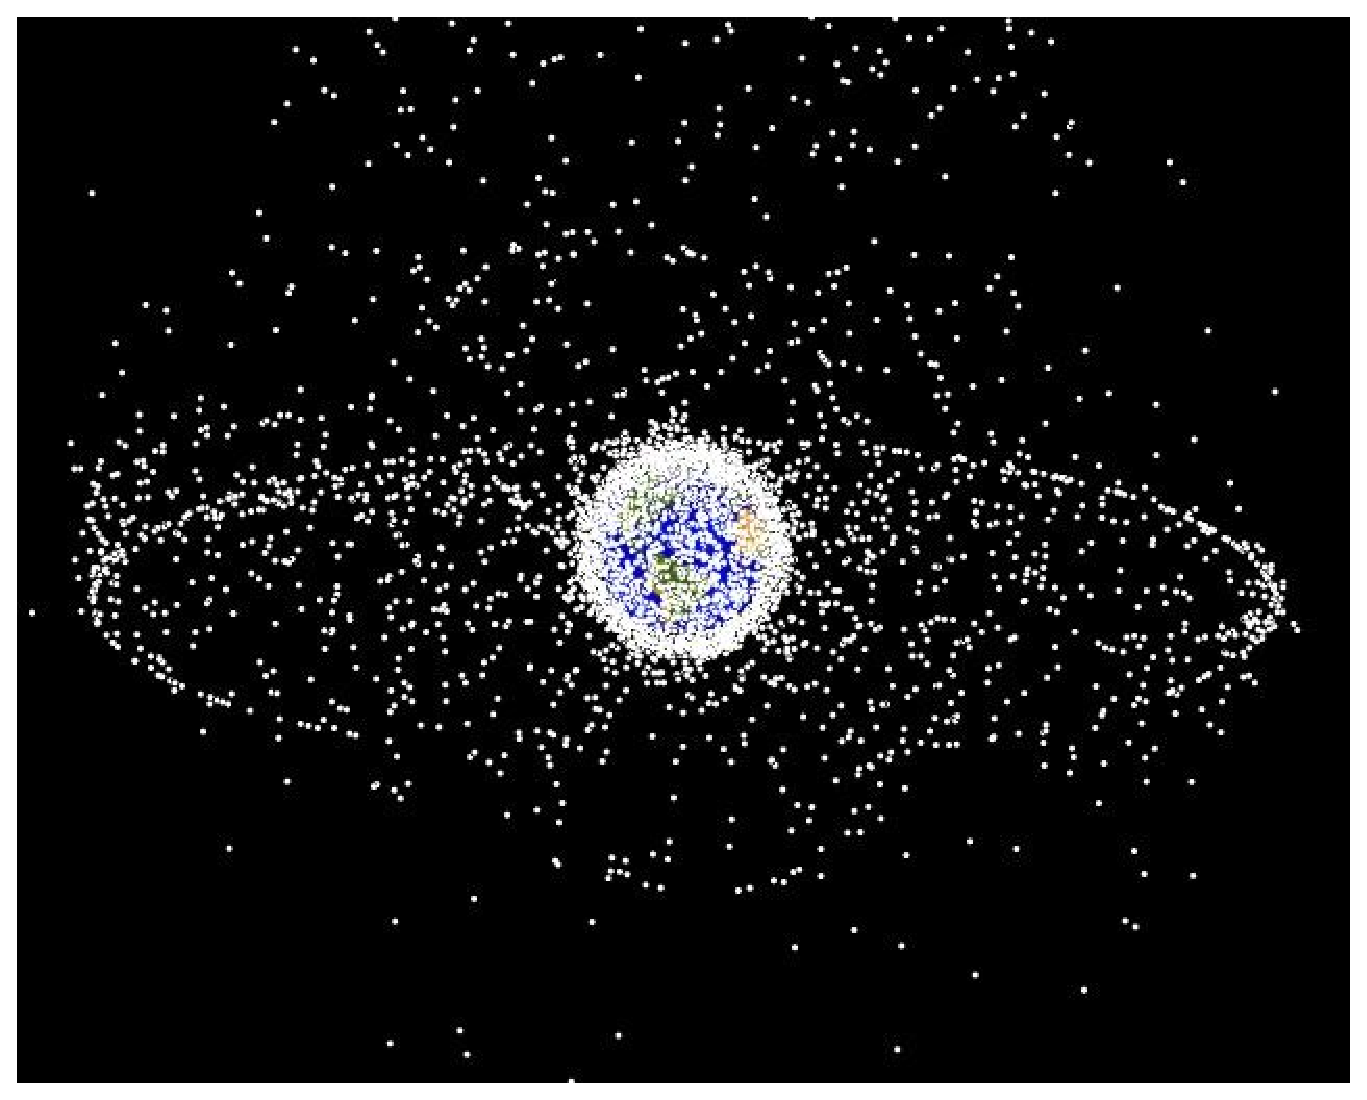
\includegraphics[width=0.8\textwidth]{eps_pics/orbitalDebris}
\caption{ Image from NASA which depicts the debris objects that are currently orbiting the Earth. Some examples of debris objects include: broken spacecraft, upper stages of launch vehicles, debris that is intentionally released from missions, debris from collisions, and paint flecks. Much of the debris seems benign due to its size but is made dangerous by its high velocity (up to 60km/s for smaller pieces).
\newline
imagesource:[http://orbitaldebris.jsc.nasa.gov/photogallery/beehives/GEO640.jpg]
	 \label{fig:orbitalDebris}} 
\end{figure}

\section{Self-Healing}

Crack healing in materials owes some of its early studies to Wool and O'Connor who modeled crack healing in polymers and experimented with cantilever beams \cite{Wool1981, Wool1982}. They found that polymer crack healing occurs in the following five stages: a) surface rearrangement, b) surface approach, c) wetting, d) diffusion, and e) randomization. Sloof, Song, and others have developed materials in which thermal activation caused a mending of cracks \cite{Song2009, Sloof2009, Bosman2009, Djugum2009, Luo2009}. Caruso et. al. reported on material strength recovery in thermoplastics by using solvent-based healing agents \cite{Caruso2009}. Inspired by the idea of biological entities being able to automatically heal wounds, a self-healing material was made by White et. al. in which a catalyst and microcapsules filled with a reactive fluid were distributed throughout a material \cite{White2001}. When the material was cracked, the capsules released their fluid which polymerized upon contacting the catalyst and effectively fused the faces of the crack together (Figure \ref{fig:selfHealingMedium}). Sottos et. al. have improved this self-healing implementation and found that damaged materials recovered up to 90\% of their original strength \cite{Sottos2009}. The White and Sottos group have also studied crack healing by introducing hardener filled microcapsules into an epoxy that was molded into a double cantilever beam fracture specimen \cite{Mcllroy2009}. This concept has been extended to a self-healing coating that contained epoxy filled microcapsules and was tested on cold rolled steel sheets with good results\cite{Zhao2012}. Manuel et. al. created a matrix containing wires that could apply a force to the material to close a crack and then the material was heated to weld the crack together \cite{Manuel2009}. Adhesives with self-healing properties have been created by Jin et. al. and tested on composite laminates where they were found to increase the life of specimens subject to fatigue \cite{Jin2009}. Self repairing chemicals have been successfully implemented on composite airplane components and were able to return to 88\% of their original strength after impact and shear testing \cite{Dry2009}. Recently, there has been a large interest in applying self-healing methods to help prolong the life of concrete which is very prone to cracks \cite{Wu2012}. 

\begin{figure}[ht!]
\centering
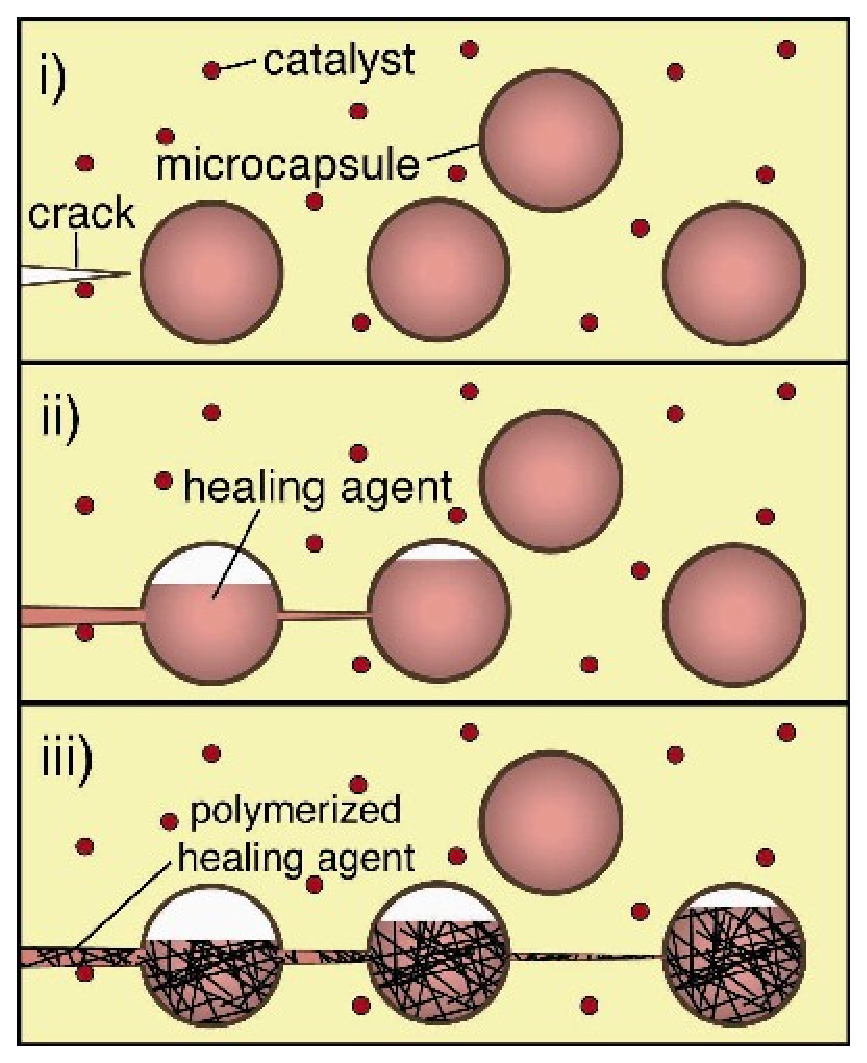
\includegraphics[width=0.5\textwidth]{eps_pics/selfHealingMedium}
\caption{ Concept drawing of a self-healing material in which microcapsules filled with a reactive fluid and a catalyst are spread throughout that material. The drawing depicts the stages of damage, fluid release, and polymerization.
\newline
source:[http://www.howstuffworks.com/self-healing-spacecraft1.htm]
	 \label{fig:selfHealingMedium}} 
\end{figure}

\section{Accelerating the Self-Healing Process}

Typically, the damaging process will continue to occur as the material attempts to mend itself together. It is therefore important that the material heals itself quickly so that the damage process does not dominate and prevent the material from reaching a full mechanical recovery. Studies have been performed on fatigue crack propagation in a self healing material \cite{Brown2003}. Sheng, Burattini, and many others reported on increasing the healing rate by improving the materials that are used \cite{Sheng2009, Burattini2009, Nakao2009, Imperiale2009, Zhang2007}. The use of U.V. light has been researched as a way to accelerate the healing process in metallopolymers and ethyl cellulose based copolymers \cite{Tang2009, Burnworth2009}. Wool and O'Connor found in their work that an increase in pressure at the crack interface during the early stages of healing or an increase in temperature at any stage can increase the rate at which the material recovers \cite{Wool1981}. Murphy et. al. have studied direct heating as a method to increase healing capabilities\cite{Murphy2009}. Direct heating to improve healing has also been applied to concrete \cite{Garcia2009, Nishiwaki2009}. Applying pressure to a crack location via acoustic energy was studied by Korde et al. both theoretically and experimentally which found that acoustic energy can accelerate the healing process \cite{Sarrazin2009, Cushman2012, Barnes2009}. Fettig et. al. have also found that healing is optimized by ensuring good mixing in the early stages which can be brought about by localized pressure \cite{Fettig2009}. Sarrazin treated cracked nylon dog-bone specimens with ultrasonic probes which increased the temperature within the specimen and caused a fusing of the crack faces  \cite{Sarrazin2-2009}. By using ultrasonic waves both the temperature and pressure at a recovery site could be increased which results in a faster healing time.

\section{Implementation}

Two main problems arise when implementing any of the previously described external stimulation methods to accelerate the healing process; i) detecting when damage has actually occurred and ii) applying the stimulation energy only to the damage location. In regards to i), it would be highly inefficient and potentially damaging to continually introduce energy if healing is not taking place. Along similar lines of reasoning, one would want only to apply energy to the actual recovery location for increased efficiency and so that unintended damage to the system does not occur. Acoustic energy is the method chosen here as it offers solutions to both problems. 

\subsection{Damage Sensing}

Picture a rod with transducers on either end that are capable of playing and recording sound. First, one transducer propagates a low energy acoustic stress-waves through the material and the other records the response of the material. If this process is repeated periodically and the response is monitored then a change in the response is observed if there is a change in the medium (e.g., damage has occurred; Figure \ref{fig:detectChange}). The acoustic energy could then be applied after this change in response has been detected and cease once the system determines that the response has returned to its initial state within some tolerance level. Imaging using ultrasonics has been around for some time now and is probably most recognized in ultrasounds that are used during pregnancy \cite{Ultrasound2006}. Ultrasonic imaging has been widely used in nondestructive testing to find cracks within structures. Harris et. al. used acoustic emission to monitor the fatigue crack growth in both aluminum and steel samples \cite{Harris1974}. Detecting cracks in concrete by using ultrasound was reported by Zinin et. al. \cite{Zinin2000}. Acoustic waves have also been used to detect cracks in very fragile materials such as eggshells \cite{DeKetelaere2000}. Recently, ultrasound has been used in dentistry to detect microcracks within teeth \cite{Matsushita2012}.

 \begin{figure}[ht!]
\begin{subfigmatrix}{2}
\subfigure[Acoustic wave propagating through medium with no defect]
{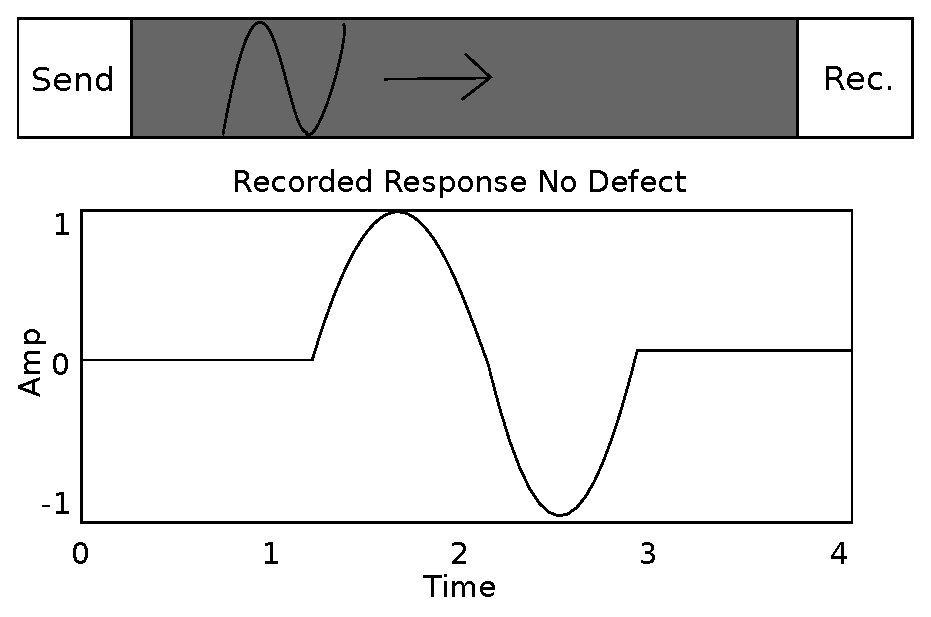
\includegraphics[width=0.5\textwidth]{eps_pics/sentNoCrack}}
\subfigure[Acoustic wave propagating through medium with a crack]
{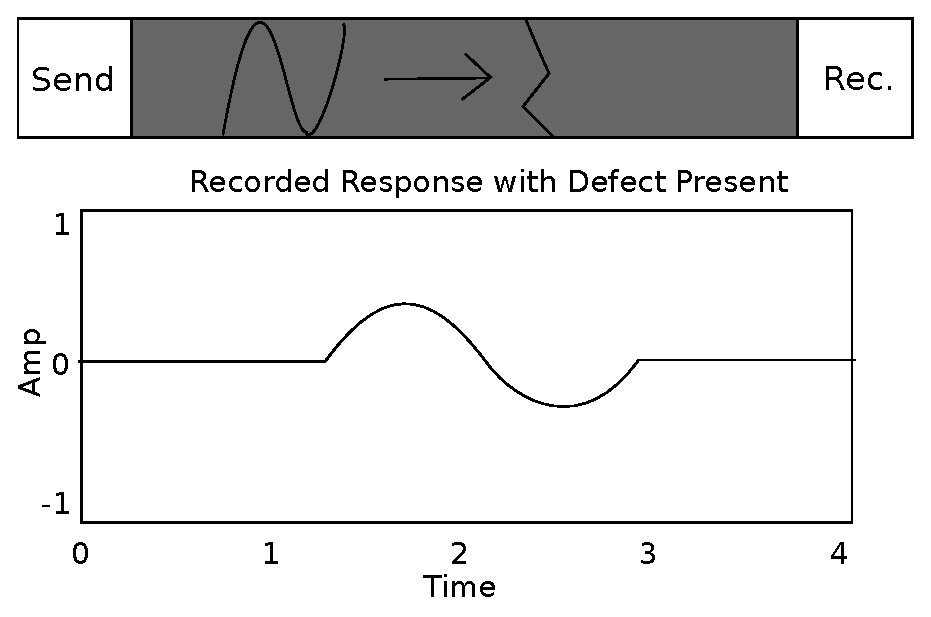
\includegraphics[width=0.5\textwidth]{eps_pics/sentCrack}}
\end{subfigmatrix}

   \caption
   { \label{fig:detectChange}
   a)A transducer sends an acoustic wave through a medium and a transducer on the opposite end records the response. This material is seen without a defect and the simulated response is shown; b) Same as a), but a defect is now present in the medium which causes a change in the response recorded on the opposite end and is seen in the simulated recorded response.
 }
\end{figure}

\subsection{Time Reversal Focusing}
Besides the mechanics of focusing the energy at the crack location, the problem arises that the location of the defect is not necessarily known. A method is needed that not only localizes the energy at the healing site but it does so without knowledge of the physical location of that site. Acoustic time reversal signal processing is one such method that possesses the aforementioned qualities. Picture again the cracked medium with transducers on either end. As before, a stress-wave is played by one transducer. This time, however, both transducers record signals. The stress-wave propagates through the medium and strikes the crack which causes the wave to split into multiple components that transmit to the opposite transducer and reflect back to the original sending transducer where they are recorded. If the transducers re-amplify and playback these signals in a time reversed fashion then the waves meet at the point where they split (here, the crack) which causes a focusing of their energy at that point. The focused wave splits again into multiple components that are recorded by each transducer and the time reversal process is repeated iteratively with a better focusing being achieved on each iteration until limits due to dissipation are reached (Figure \ref{fig:trDrawing} illustrates this concept). The time reversal concept can be extended to multiple dimensions in which the transducers are placed around the boundary. In a self-healing material, the focusing of energy at a crack location would accelerate the healing process at that site.

\begin{figure}[ht!]
\centering
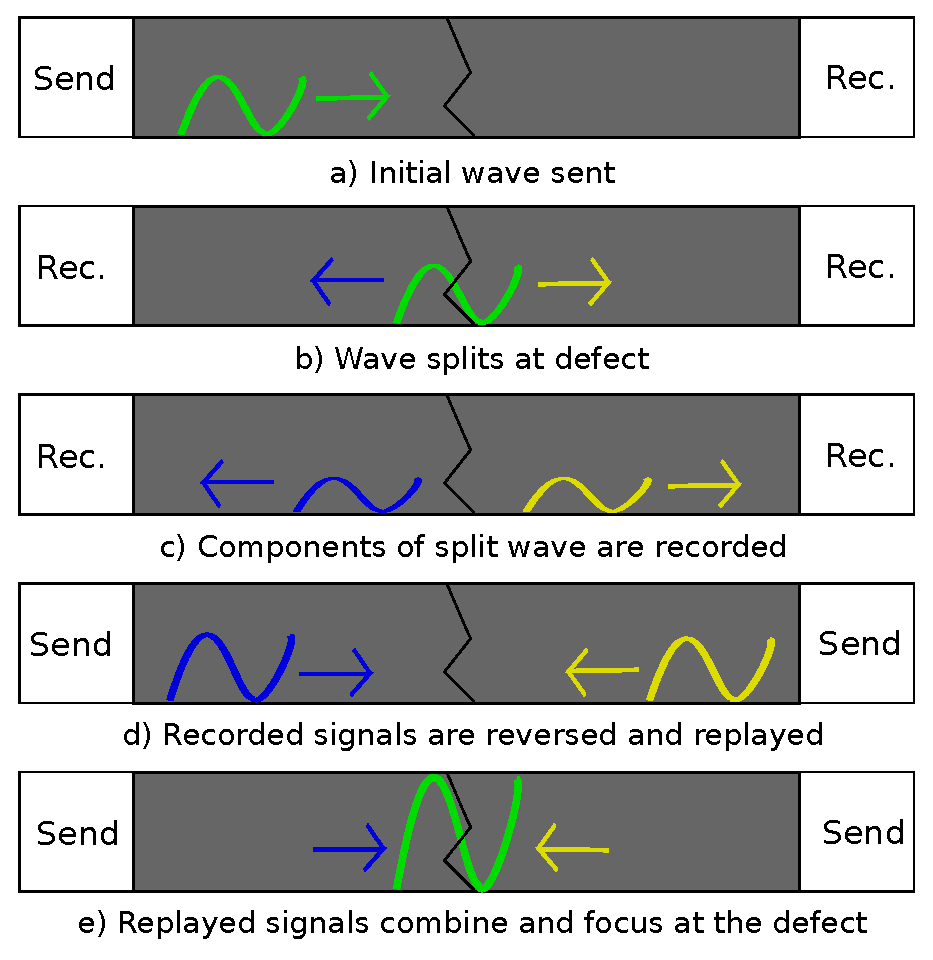
\includegraphics[width=0.7\textwidth]{eps_pics/trDrawing}
\caption{ Concept drawing of time reversal in one dimension; a) An initial wave is sent out by a transducer; b) The wave travels down the rod until it hits the crack and splits into multiple components; c) The components of the incident wave travel towards each transducer where they are recorded; d) The recorded signals are amplified and replayed in a time reversed fashion; e) The wave components simultaneously reach the crack location where they first split and combine to cause a focusing of their amplitude at that point.
	 \label{fig:trDrawing}} 
\end{figure}

Mathematically, time reversal is the time domain analog of phase conjugation which has been used in adaptive optics to correct for wavefront phase aberrations by forming a mirror to produce the conjugate phase aberrations of the incoming wave which results in a corrected wavefront \cite{Pepper1982}. Acoustic time reversal has been studied extensively by Fink et. al. in which he first setup an array of transducers to send and receive ultrasonic waves through a rubber medium with random thicknesses and a hydrophone embedded as a reflector/receiver.  Fink also has shown iterative focusing by experimenting with an array of transducers and two metal wires as reflectors. In the iterative experiments, it was shown that the energy focused on the strongest reflector after successive iterations \cite{Fink1993}. Experiments were performed by Derode et. al. in which a transducer played a signal through a liquid containing over 2000 rods and an array of transducers located on the opposite side of the rods played the captured signals back and it was found that the replayed signals converged on the original source \cite{Derode1995}. Time reversal has been applied to acoustic communications in both the ocean and air to achieve better signal to noise ratio by focusing the signal at the desired receiver \cite{Smith2003, Song2012, Shimura2012}. Great promise has also been shown with applying time reversal to biomedical application such as the focusing of ultrasonic waves to destroy kidney stones or hyperthermia brain treatment \cite{Fink2003}. The concept of time reversal is not only applicable to acoustics but can also be used with electromagnetic waves \cite{Lerosey2004}. Liu et. al. have shown experimentally that bit-rate-errors in radio communications can be reduced by applying time reversal \cite{Liu2008}. MIT has effectively created a microwave cannon by using the time reversal process to focus microwave energy \cite{Davy2010}.

\section{Objectives}
The overall goal, as devised by Dr. Korde, is to use time reversal acoustic focusing to accelerate the crack recovery process of a self-healing polymer by locally increasing the temperature and pressure. The work presented here looks at a subsection of that project which is the time reversal focusing at a crack location. There has been much theoretical and experimental work performed on applying time reversal in multiple dimensions. Here, the case of time reversal in one dimension is explored. Fouque et. al. performed calculations and simulations on one dimensional time reversal in random media with an embedded reflector to determine the reflector's location \cite{Fouque2006}. Korde performed calculations on focusing at a crack with piezoelectric transducers and time reversal processing \cite{Fehrman2012}. To the author's knowledge, time reversal focusing at a defect location in one dimension has not been performed experimentally. In this work experiments are performed on circular steel and nylon rods with piezoelectric transducers to send and receive signals. This could have direct applications to the rods used in deployable space structures that may become cracked over time. Although the analysis is eased in this scenario, there are difficulties introduced in performing the experiments in one dimensional structures of finite length that are not present when performing time reversal in multiple dimensions. For instance, it is required that a transducer both sends a signal and reads a signal in the same iteration such that the ringing of the transducer may interfere with the signal being read.\newline

The specific objectives of this work are to show:
\begin{enumerate}
\item Modeling and experimental verification of acoustic time reversal crack focusing in one dimension
\item Experimental verification of acoustic crack detection in one dimension
\item Experimental verification of iterative focusing and convergence of acoustic time reversal crack focusing in one dimension
	\begin{enumerate} 
	\item Show that with each iteration, the amplitude seen at the defect increases until a convergence point is reached
	\end{enumerate}

\end{enumerate} % You may enter in the file or directly here.

\chapter{Modeling}\label{ch:Modeling}
% Modeling
This chapter begins with the models and derivations for the case of one dimensional time reversal and is based upon work performed by Korde \cite{Fehrman2012}. Following that material will be a brief overview of two dimensional time reversal which is drawn from a number of published sources.

\section{One Dimensional Wave Equation}
\label{sec:oneDWaveEquation}

In this section the one dimensional wave equation for a linear elastic material with uniform density and cross-sectional area will be derived. The derivation is based on knowledge from numerous books such as Kolsky \cite{Kolsky1963} and Brown et. al. \cite{Brown2008}.

\begin{figure}[ht!]
\centering
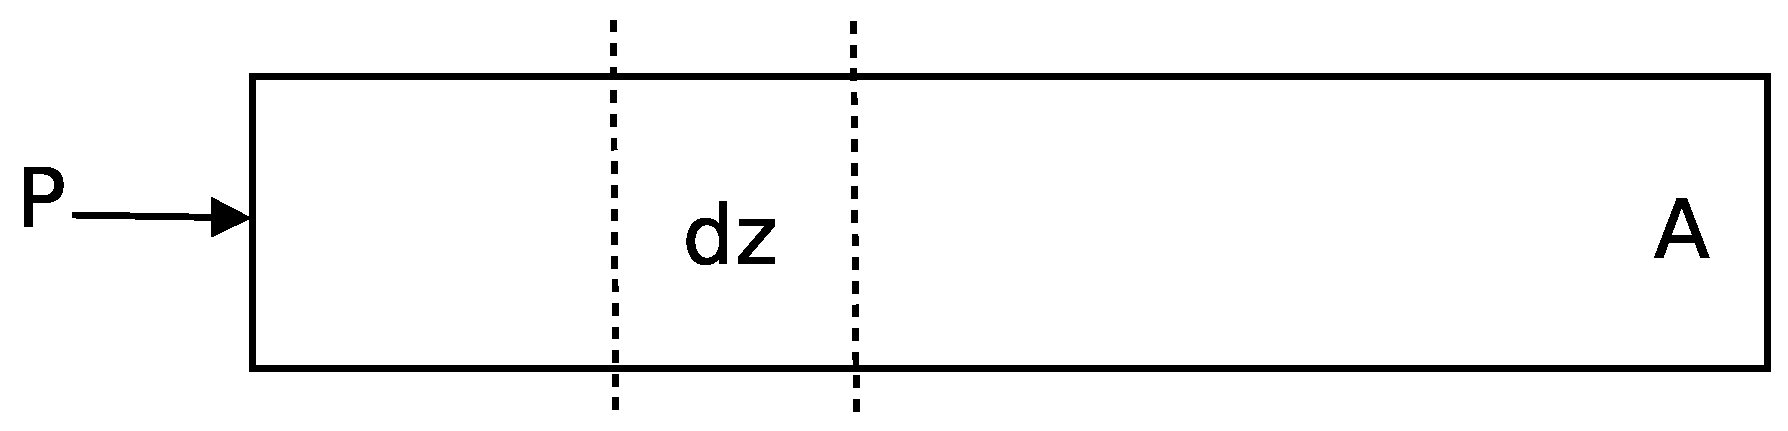
\includegraphics[width=0.8\textwidth]{eps_pics/deriveWaveRod}
\caption{Diagram for deriving the one dimensional wave equation given an axial pressure applied to one end of the material with uniform density and cross-sectional area.
	 \label{fig:deriveWaveRod}} 
\end{figure}

Figure \ref{fig:deriveWaveRod} gives a basic diagram that is used for the wave equation derivation, with $P$ being the axial pressure, $dz$ being the material's differential element of length, and $A$ being the cross-sectional area of the material. Define the stress in the z direction as:

\begin{equation}
T_3 = \frac{P}{A}
\end{equation}

\nomenclature{$P$}{Axial pressure applied to rod end}
\nomenclature{$A$}{Cross-sectional area of the rod}
\nomenclature{$dz$}{Differential element of length for the rod}
\nomenclature{$T_3$}{Stress in the z direction}

\begin{figure}[ht!]
\centering
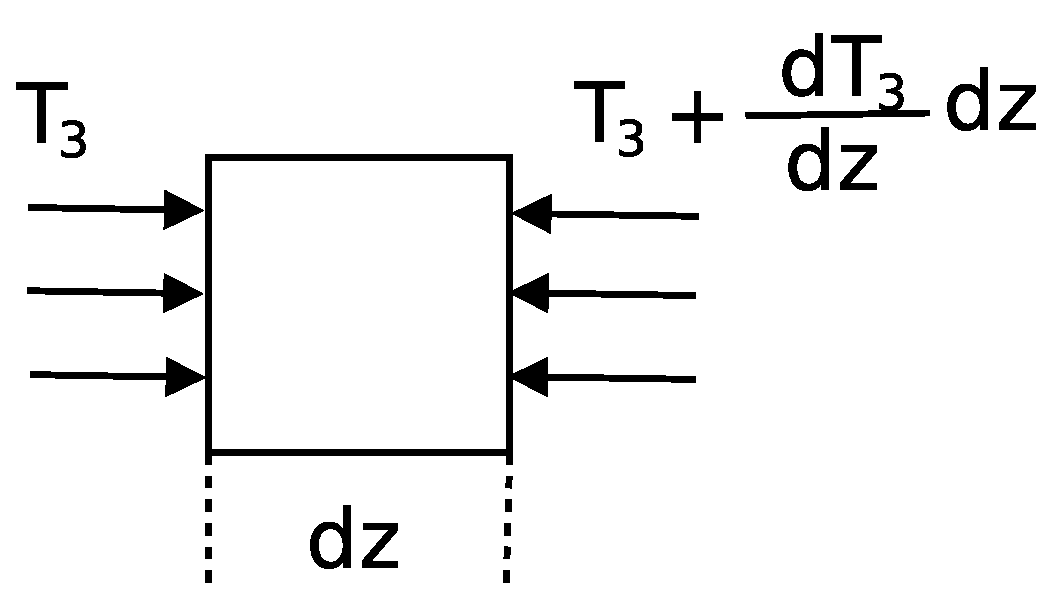
\includegraphics[width=0.8\textwidth]{eps_pics/diffElementRod}
\caption{Differential element showing the stresses acting on the rod.
	 \label{fig:diffElementRod}} 
\end{figure}

Applying Newton's second law and summing the forces,

\begin{equation}
-T_3A + (T_3 + \frac{dT_3}{dz}dz)A = A\rho^* dz \frac{d^2w}{dt^2}
\end{equation}

\nomenclature{$\rho^*$}{Density of the rod material}
\nomenclature{$w$}{Displacement of the rod}

With $\rho^*$ being the density of the rod material and $w$ being the displacement. Dividing through by the area,

\begin{equation}
-T_3 + T_3 + \frac{dT_3}{dz}dz = \rho^* dz \frac{d^2w}{dt^2}
\end{equation}

\begin{equation}
\frac{dT_3}{dz}dz = \rho^* dz \frac{d^2w}{dt^2}
\end{equation}

Canceling the $dz$ term,

\begin{equation}
\frac{dT_3}{dz} = \rho^* \frac{d^2w}{dt^2}
\label{eq:strainWave}
\end{equation}

$C^*_{33}$ is the elastic constant in the z direction and is defined as the ratio of the stress and strain in the z direction. This is given by,

\begin{equation}
C^*_{33} = \frac{T_3}{S_{33}} \implies T_3 = C^*_{33}S_{33}
\label{eq:T_3}
\end{equation}

\nomenclature{$C^*_{33}$}{Elastic constant in the z direction}
\nomenclature{$S_{33}$}{Strain in the z direction}

With $S_{33}$ being the strain in the z direction. Strain is the ratio of the change in material length to the original length and in this case is given by,

\begin{equation}
S_{33} = \frac{dw}{dz}
\label{eq:S_33}
\end{equation}

Inserting \ref{eq:S_33} in to \ref{eq:T_3} we see that

\begin{equation}
T_3 = C^*_{33}\frac{dw}{dz}
\label{eq:T_3fin}
\end{equation}

Putting \ref{eq:T_3fin} back in to \ref{eq:strainWave} and realizing that $w$ is a function of both $t$ and $z$,

\begin{equation}
C^*_{33}\frac{\partial ^2w}{\partial z^2} = \rho^* \frac{\partial ^2w}{\partial t^2}
\end{equation}

Dividing through by $\rho^*$ and moving the LHS term to the RHS, we arrive at

\begin{equation}
\frac{\partial ^2w}{\partial t^2} - c^{*2} \frac{\partial ^2w}{\partial z^2} = 0
\label{eq:waveEquationFin}
\end{equation}

\nomenclature{$c^*$}{Velocity of wave propagation through the rod}

With $c^*$ being the velocity of the wave propagation and is defined as,

\begin{equation}
c^* = \sqrt{\frac{C^*_{33}}{\rho^*}}
\end{equation}

\section{Piezoelectric transducers}

This section describes the governing equations for $d_{33}$ piezoelectric transducers that are placed on each end of a rod. The following work is based on derivations by Dr. Korde.

The constitutive equations for the transducers are:

\begin{equation}
T_3 = \overline{C_{33}} S_3 + \overline{d_{33}} D_3
\end{equation}

and 

\begin{equation}
D_3 = \overline{\epsilon ^T_{33}} E_3 + \frac{d_{33}}{s^E_{33}} S_3
\end{equation}

Where $D_3$, $E_3$, and $d_{33}$ are the electric displacement, electric field intensity, and the strain constant relating strain and field intensity, respectively, all in the z direction. The other variables are given by the following equations:

\begin{equation}
s^E_{33} = \frac{1}{C_{33}}
\end{equation}

\begin{equation}
\overline{C_{33}} = \frac{1}{s^E_{33}(1 - \frac{d^2_{33}}{s^E_{33}\epsilon ^T_{33}})}
\end{equation}

\begin{equation}
\overline{d_{33}} = -\frac{d_{33} / \epsilon ^T_{33}}{s^E_{33}(1 - \frac{d^2_{33}}{s^E_{33}\epsilon ^T_{33}})}
\end{equation}

\begin{equation}
\overline{\epsilon ^T_{33}} = -\frac{\epsilon ^T_{33}}{s^E_{33}(1 - \frac{d^2_{33}}{s^E_{33}\epsilon ^T_{33}})}
\end{equation}

With $C_{33}$ and $\epsilon ^T_{33}$ being the PZT elastic constant in the z direction and permittivity constant in the z direction respectively.

\begin{figure}[ht!]
\centering
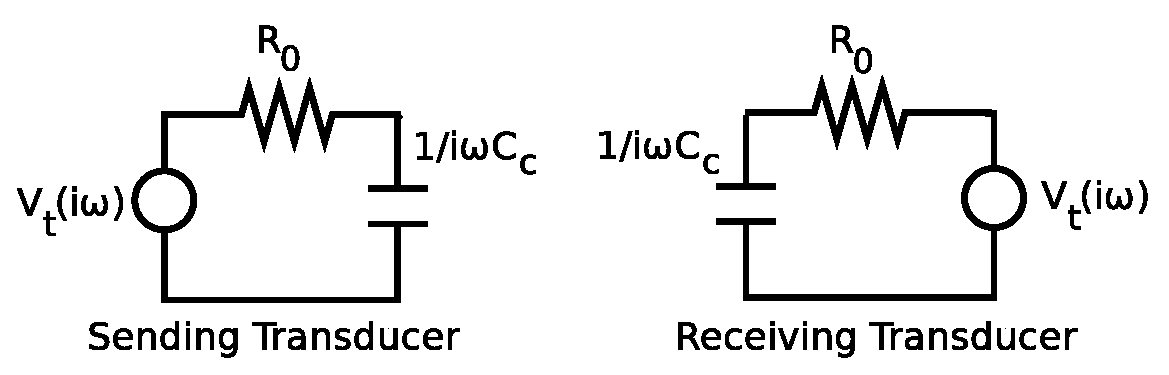
\includegraphics[width=1\textwidth]{eps_pics/trans_circ}
\caption{Equivalent circuit diagram for the piezoelectric transudcers.
	 \label{fig:trans_circ}} 
\end{figure}

The equivalent circuits for the transducers are modeled as a resistor and capacitor in series as shown in Figure \ref{fig:trans_circ} and with $C_c$ being the equivalent capacitance and is given by

\begin{equation}
C_c = \overline{\epsilon_{33}} \pi a^2/l
\end{equation}

Where $a$ and $l$ are the transducer area and length respectively. 

\section{Rod with Transducers}

\begin{figure}[ht!]
\centering
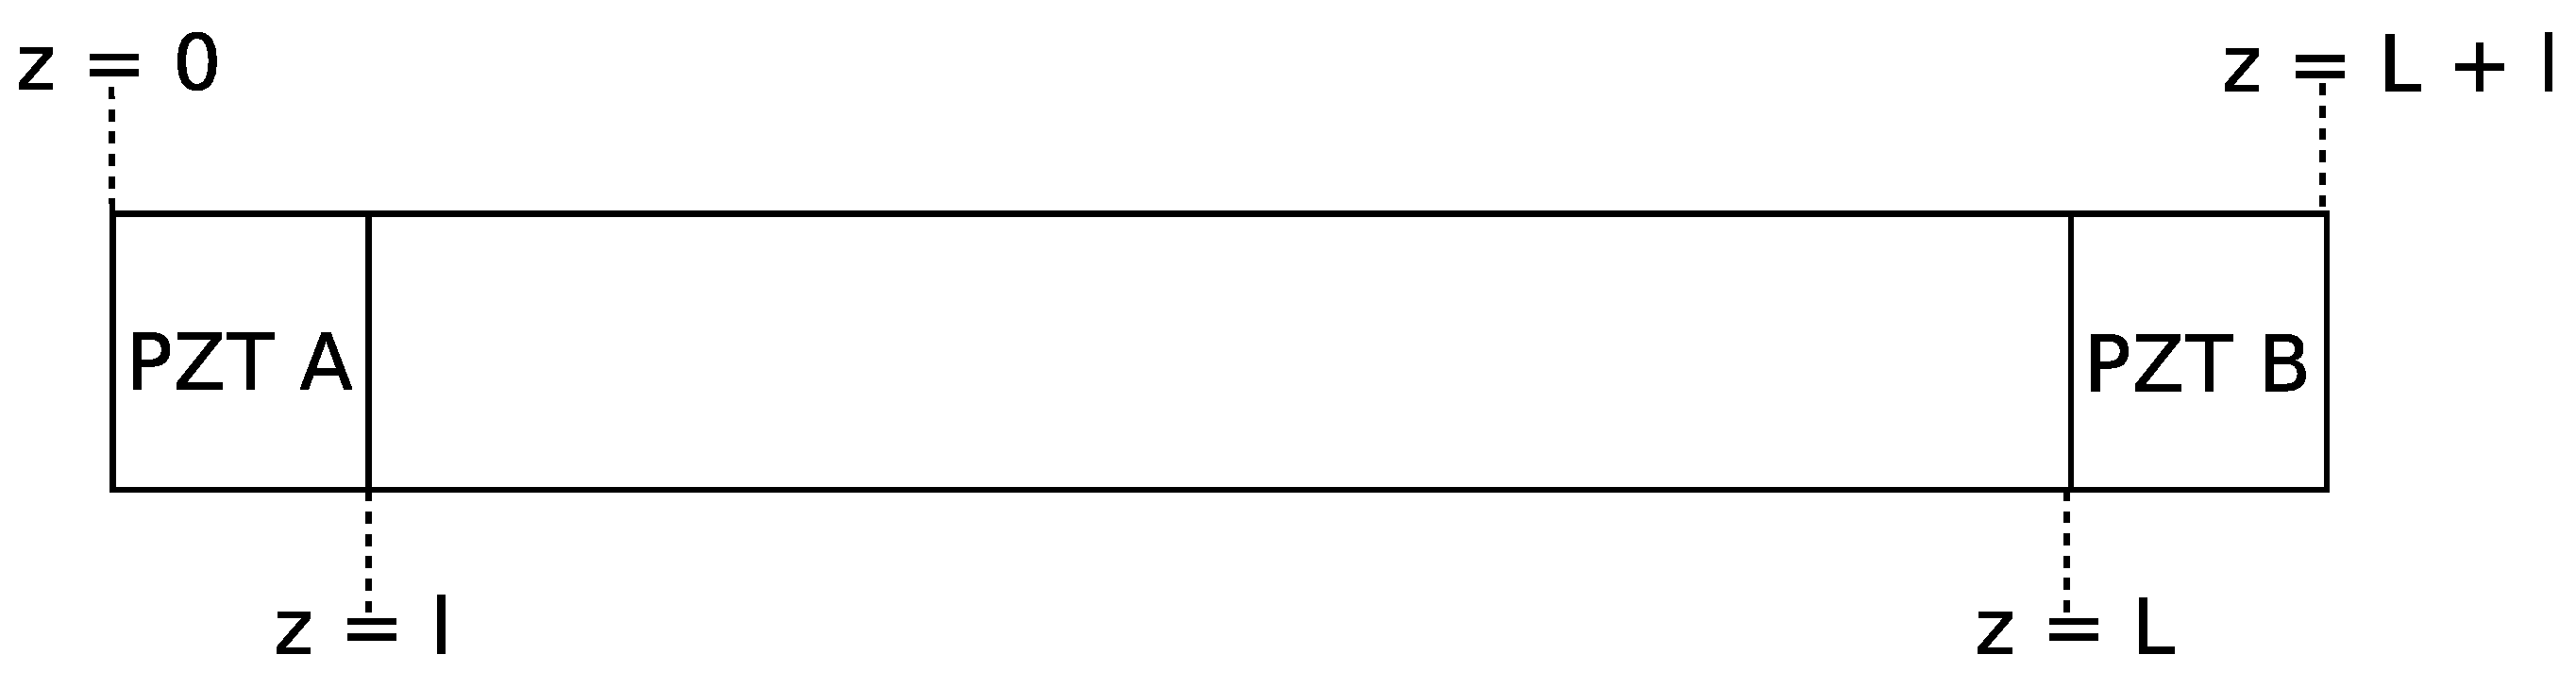
\includegraphics[width=0.8\textwidth]{eps_pics/rodTrans.eps}
\caption{Diagram of a rod with $d_{33}$ piezoelectric transducers placed on each end.
	 \label{fig:rodTrans}} 
\end{figure}

Consider a rod with $d_{33}$ transducers affixed to each end as pictured in Figure \ref{fig:rodTrans}. We wish to model propagation of a wave through the system with the wave being sent by one of the transducers. The one-dimensional wave results from Section \ref{sec:oneDWaveEquation} can be applied here such that the equation of the motion for the wave propagating through transducers is the same as through the rod but with a different density and elastic coefficient which will be denoted as $\rho$ and $C_{33}$ respectively. Then for $0 \le z \le l$ and $L < z \le (L+l)$ we have

\begin{equation}
\frac{\partial ^2w}{\partial t^2} - c^2 \frac{\partial ^2w}{\partial z^2} = 0
\label{eq:transWaveEquationFin}
\end{equation}




\chapter{Experiments}\label{ch:Experiments}
%Experiments

This chapter describes the experiments that were carried out to investigate the different components of one dimensional time reversal focusing at a defect location which is at an a prior unknown location. The components investigated include: i) detecting that a crack as occurred within the rod, ii) comparing theory to experiment for the interrogatory phase and for the first iteration of time reversal focusing, and iii) iterative focusing to achieve better a response at the defect until convergence is reached. All of the hardware and algorithms used are detailed. Code samples are given in the appendices.

\section{Hardware and Software}
The main access point to the system was a desktop pc which ran Windows XP and acted as the host computer. The power house of the entire system was a National Instruments 7853R FPGA card. This FPGA card was of PXI form factor and was housed in an NI proprietary PXI chassis which was linked to the PC via MXI cable (Figure \ref{fig:fpgaCard}). The PC contained a PCI-E card that allowed for the MXI connection. LabVIEW software with the extra real-time and FPGA modules was used to compile write and compile programs on the Windows PC. Once written and compiled to VHDL code the programs were then downloaded to the FPGA card over the MXI connection. The program execution is such that a host program runs on the desktop PC and communicates with the program running on the remote FPGA card. The time critical processes such as signal acquisition and playback are performed using the FPGA whereas the tasks that could take an arbitrary amount of time were executed on the desktop PC. The FPGA card does not provide a large amount of current and it was necessary to amplify the output signals using op-amp amplifier circuits which were capable of providing up to $30 VPP$ at $200 kHz$ (Figures \ref{fig:oneAmp} and \ref{fig:ampBox}). The interfacing of the data acquisition cables to the FPGA card was handled using an NI SCB-60 input/output box which provided screw terminal connections inside of a shielded box (Figure \ref{fig:ioBox}). The entire hardware hierarchy is shown in Figure \ref{fig:hardwareComm}. Finally, all of the data was imported into MATLAB.

\begin{figure}[ht!]
\centering
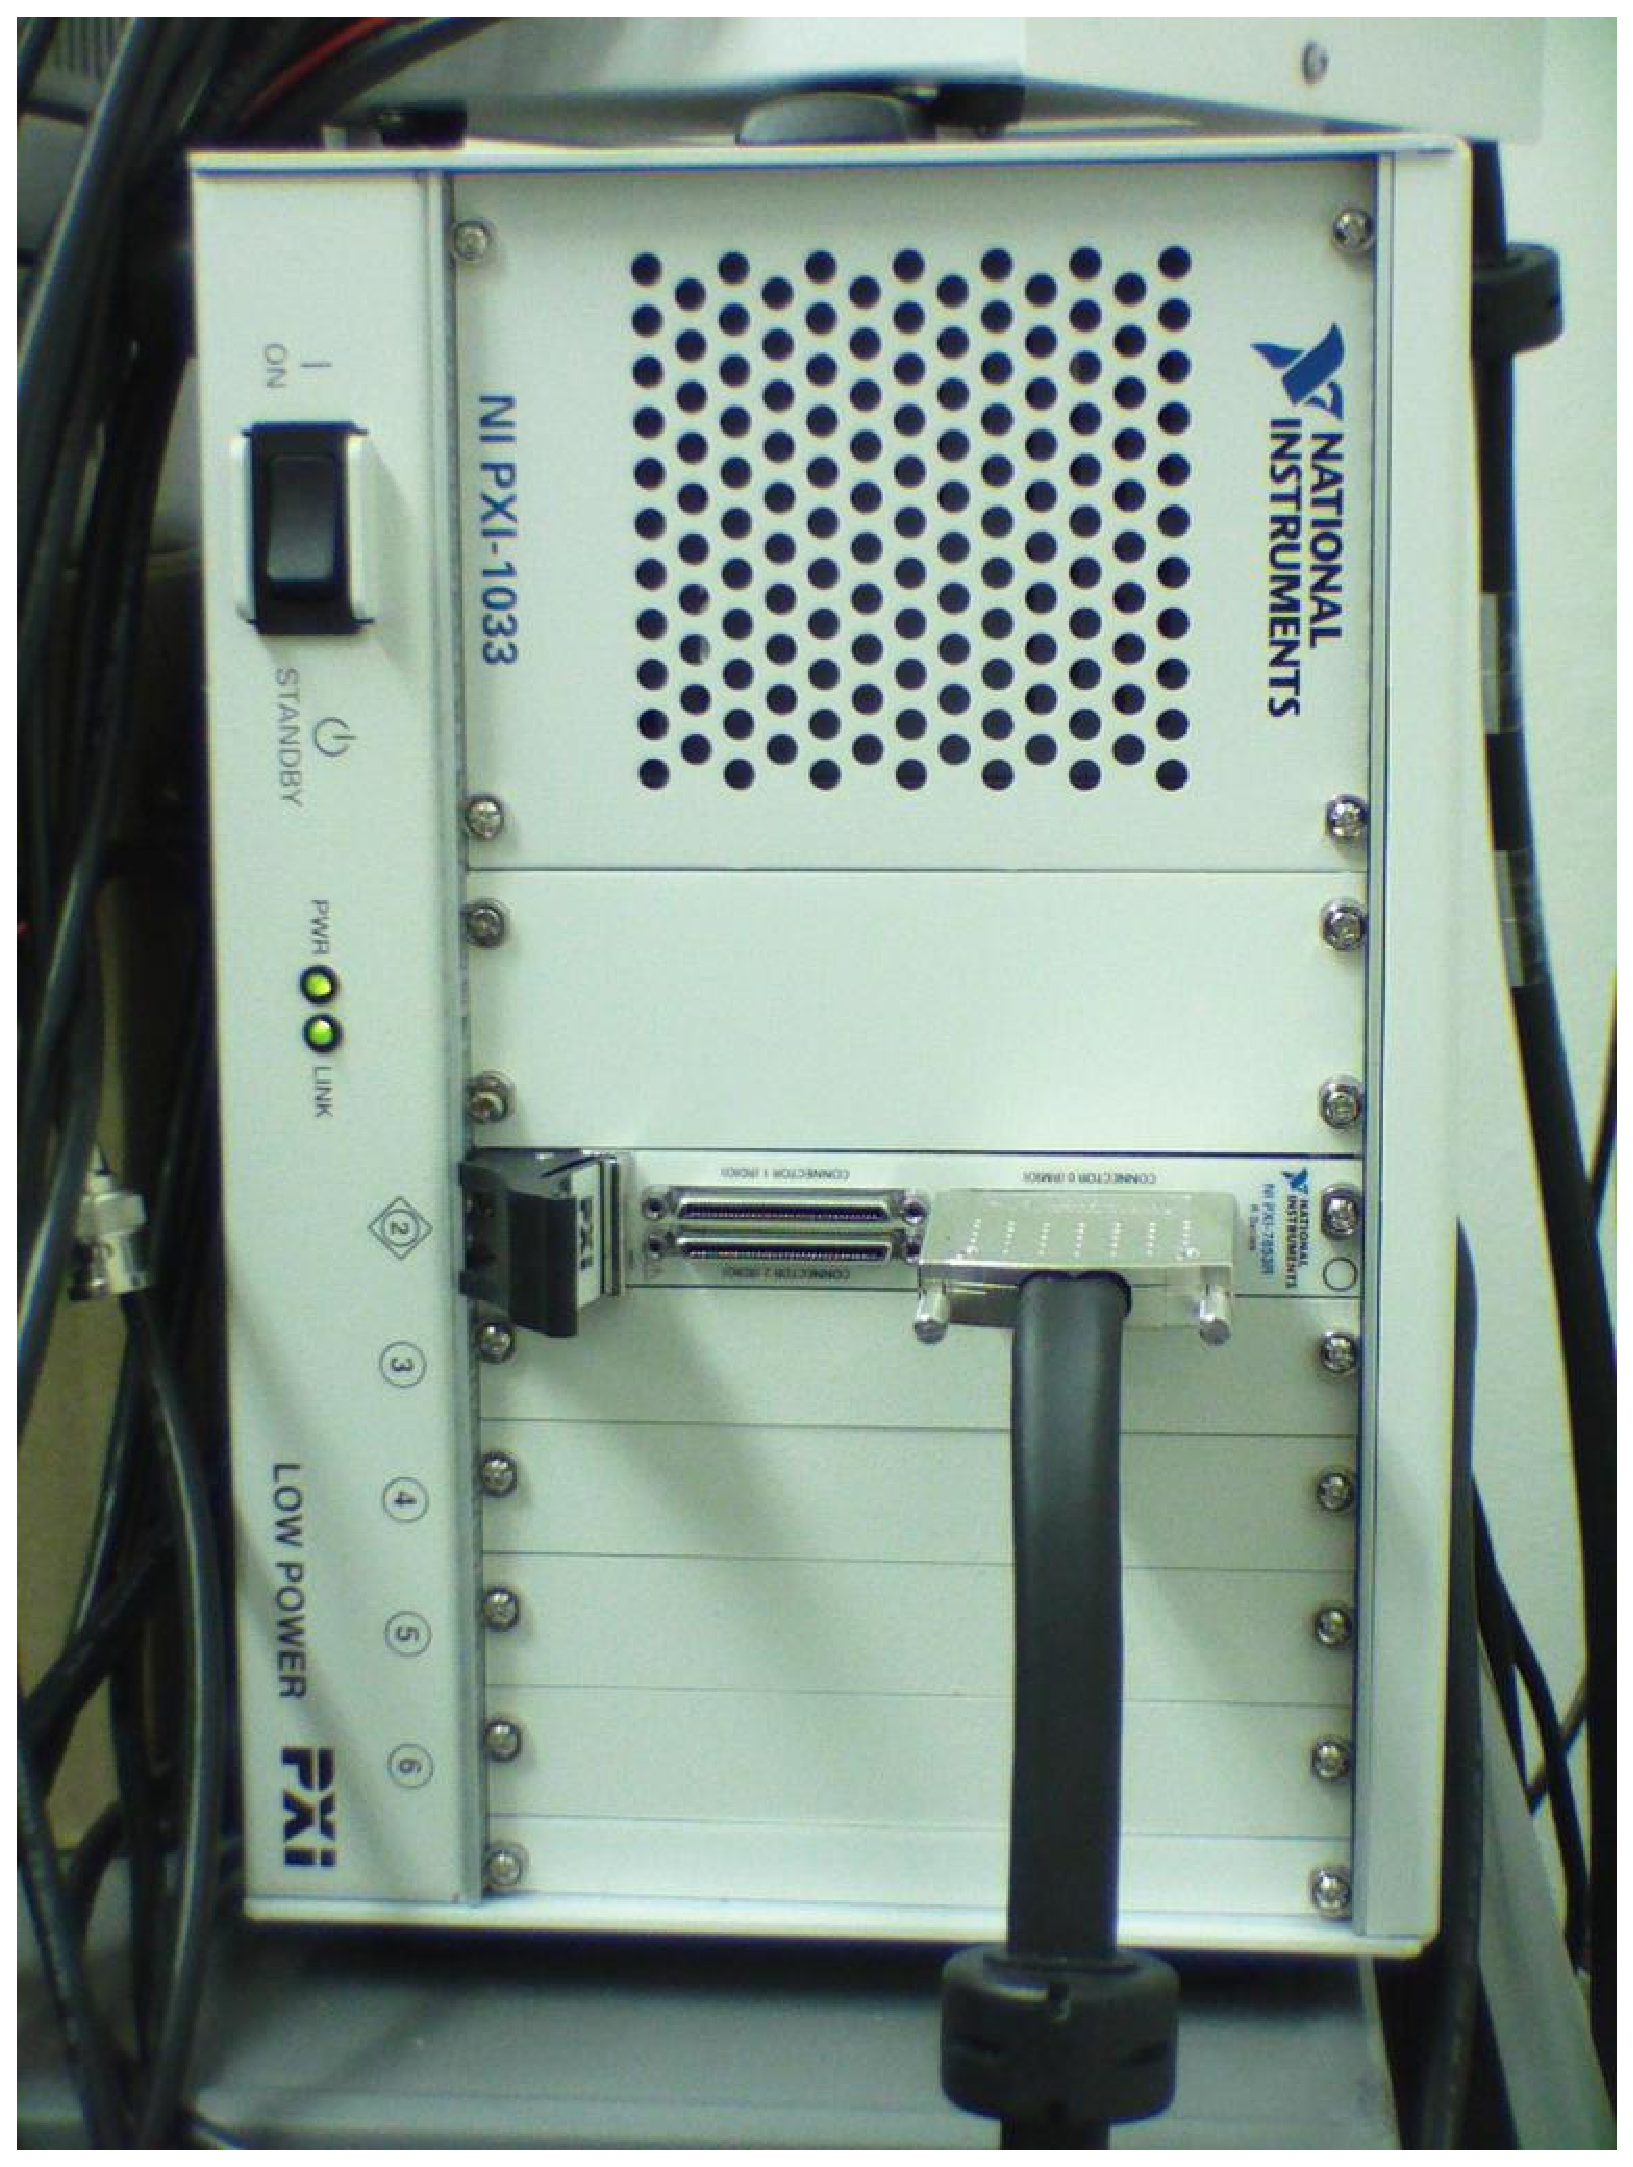
\includegraphics[width=0.6\textwidth]{eps_pics/fpgaCard}
\caption{National Instruments PXI chassis which contains the 7853R FPGA card. The 7853R is a very powerful card with a large amount of programming flexibility due to the fact that it can be programmed using a graphical language (LabVIEW) instead of needing to code directly in VHDL which can be cumbersome.
	 \label{fig:fpgaCard}} 
\end{figure}

\begin{figure}[ht!]
\centering
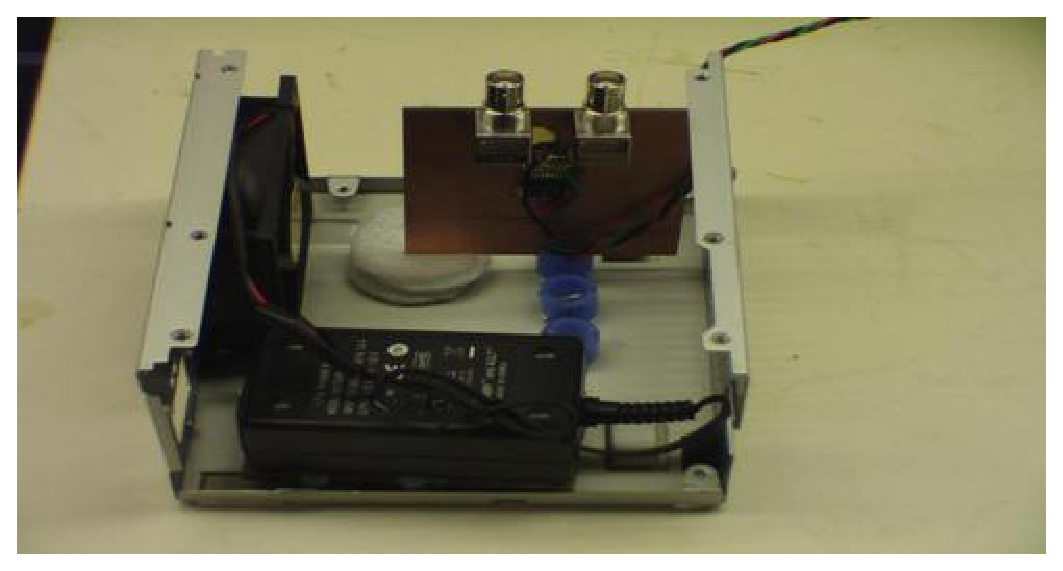
\includegraphics[width=0.7\textwidth]{eps_pics/oneAmp}
\caption{Single amplifier circuit being placed into the custom enclosure that was built from a PC power supply casing. Many thanks go to Miles Wickersham and Andy Downs for their help with designing the circuits.
	 \label{fig:oneAmp}} 
\end{figure}

\begin{figure}[ht!]
\centering
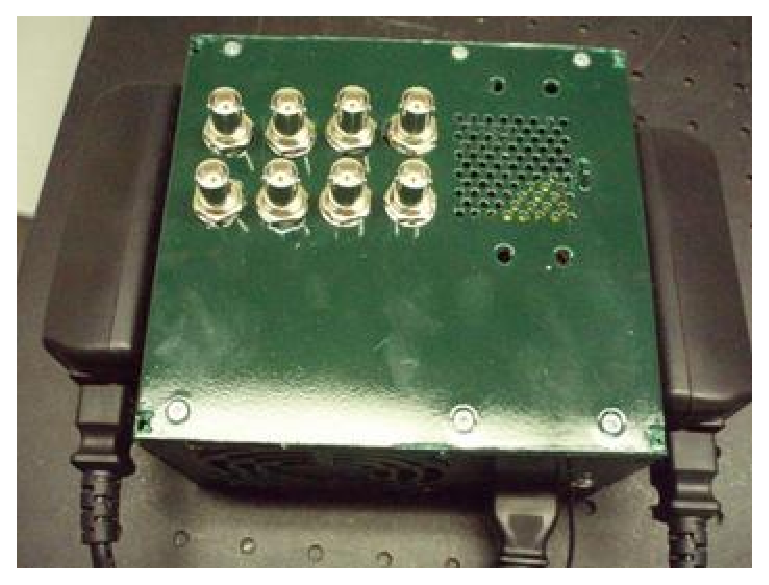
\includegraphics[width=0.7\textwidth]{eps_pics/ampBox}
\caption{Completed amplifier box containing four op-amp amplifier circuits with BNC input and output
	 \label{fig:ampBox}} 
\end{figure}

\begin{figure}[ht!]
\centering
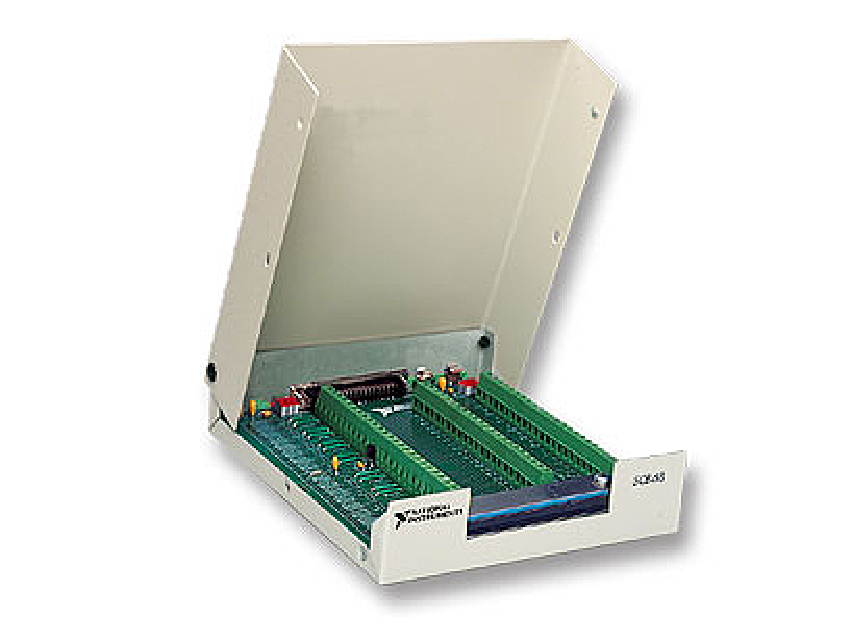
\includegraphics[width=0.7\textwidth]{eps_pics/ioBox}
\caption{NI SCB-60 shielded input/output box that is used for interfacing electrical connections to the 7853R FPGA card. \newline source:www.ni.com
	 \label{fig:ioBox}} 
\end{figure}

\begin{figure}[ht!]
\centering
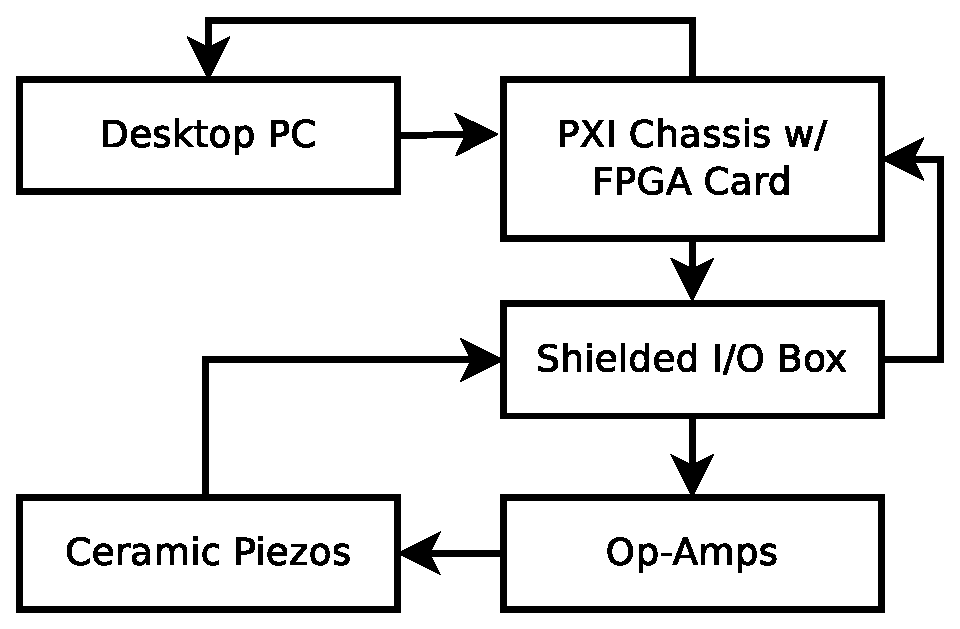
\includegraphics[width=0.7\textwidth]{eps_pics/hardwareComm}
\caption{Diagram which shows the communication hierarchy among the different hardware pieces that were used for testing. The communication between the PC and FPGA card was performed using a MXI cable. The acquisition cables interfaced to the FPGA through an NI shielded I/O box and cable. Any other connections were made using normal insulated copper wire.
	 \label{fig:hardwareComm}} 
\end{figure}

\section{Crack Detection Tests}

The first topic investigated is if the system is able to sense when a defect has become present within the material. This step is important because it would be inefficient and potentially damaging to attempt to perform acoustic focusing when no defect is present in the system.

The setup used for the crack detection involved the use of both nylon and steel solid circular rods. Each rod was approximately $12.7 \times 10^{-3} m$ in diameter. The steel rod was tested first and found to have a density of $7.894 \times 10^3 kg/m^3$, an elastic constant of $169.39 \times 10^9 N/m^2$, and a length of $579 \times 10^{-3} m$. The actuators used to send and receive the signals were piezoceramic stack actuators (PZT) with a diameter of $13 \times 10^{-3} m$ with a piezoelectric strain constant of $d_{33} = 152 \times 10^{-12} C/N$ and a relative permittivity of $\epsilon _{33} = 450 \epsilon _0$ with $\epsilon _0 = 8.854 \times 10 ^{-12} F/m$. Two transducers were affixed to each end of the steel rod using accelerometer putty with PZT A being on the left side of the rod and PZT B being on the right side. This system was then placed into compression using a custom built mechanism. The compression mechanism was created using common nuts and bolts, optics table hardware, and a few machined aluminum blocks (Figure \ref{fig:compression}). The compression could be controlled by the use of a single bolt and was tightened with a small screw driver to one-quarter turn past being finger tight. The experiments were carried out on an optics table which significantly reduced external vibrations through the use of air damping. The setup is shown in Figure \ref{fig:steelUncrackedFull}. Also pictured in the setup is a terminal block that was used for handling the copper wire connections (Figure \ref{fig:junctionBox}). The terminal block also contains a diode circuit consisting of two diodes that is placed between the amplifier output lines and the analog read in lines for each PZT (Figure \ref{fig:diodeCircuit}). The diode circuit snuffs out noise from the amplifier that was found to be large enough to overshadow some test results and will be discussed more in the results section.

\begin{figure}
\begin{subfigmatrix}{2}
\subfigure[Left side compression mechanism]
{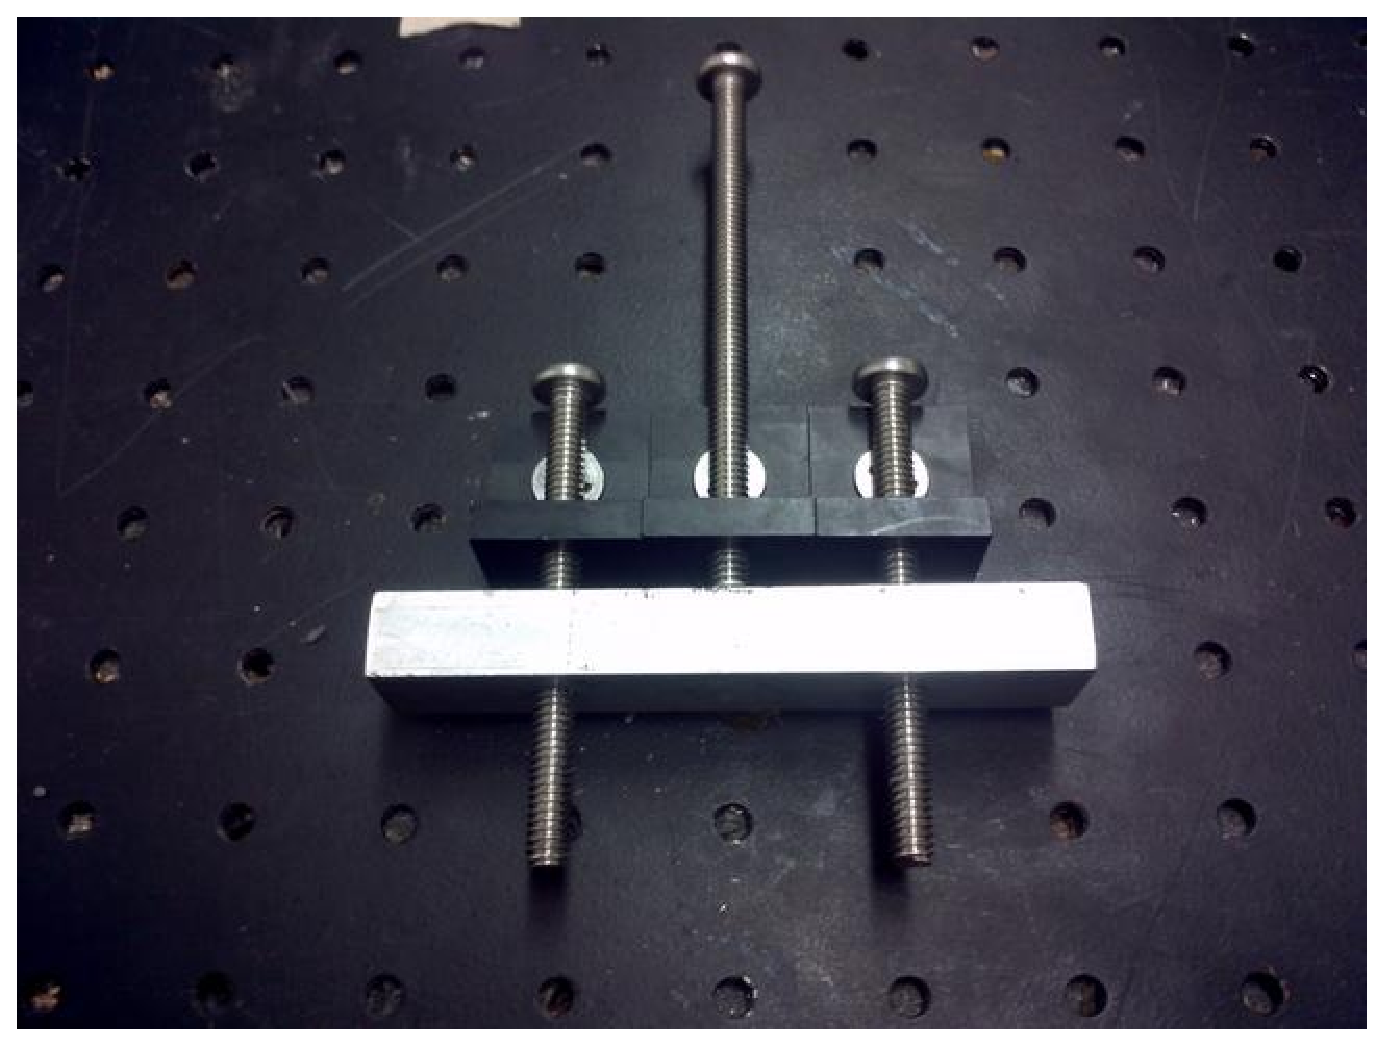
\includegraphics[width=0.7\textwidth]{eps_pics/lsCompression}}
\subfigure[Right side compression mechanism ]
{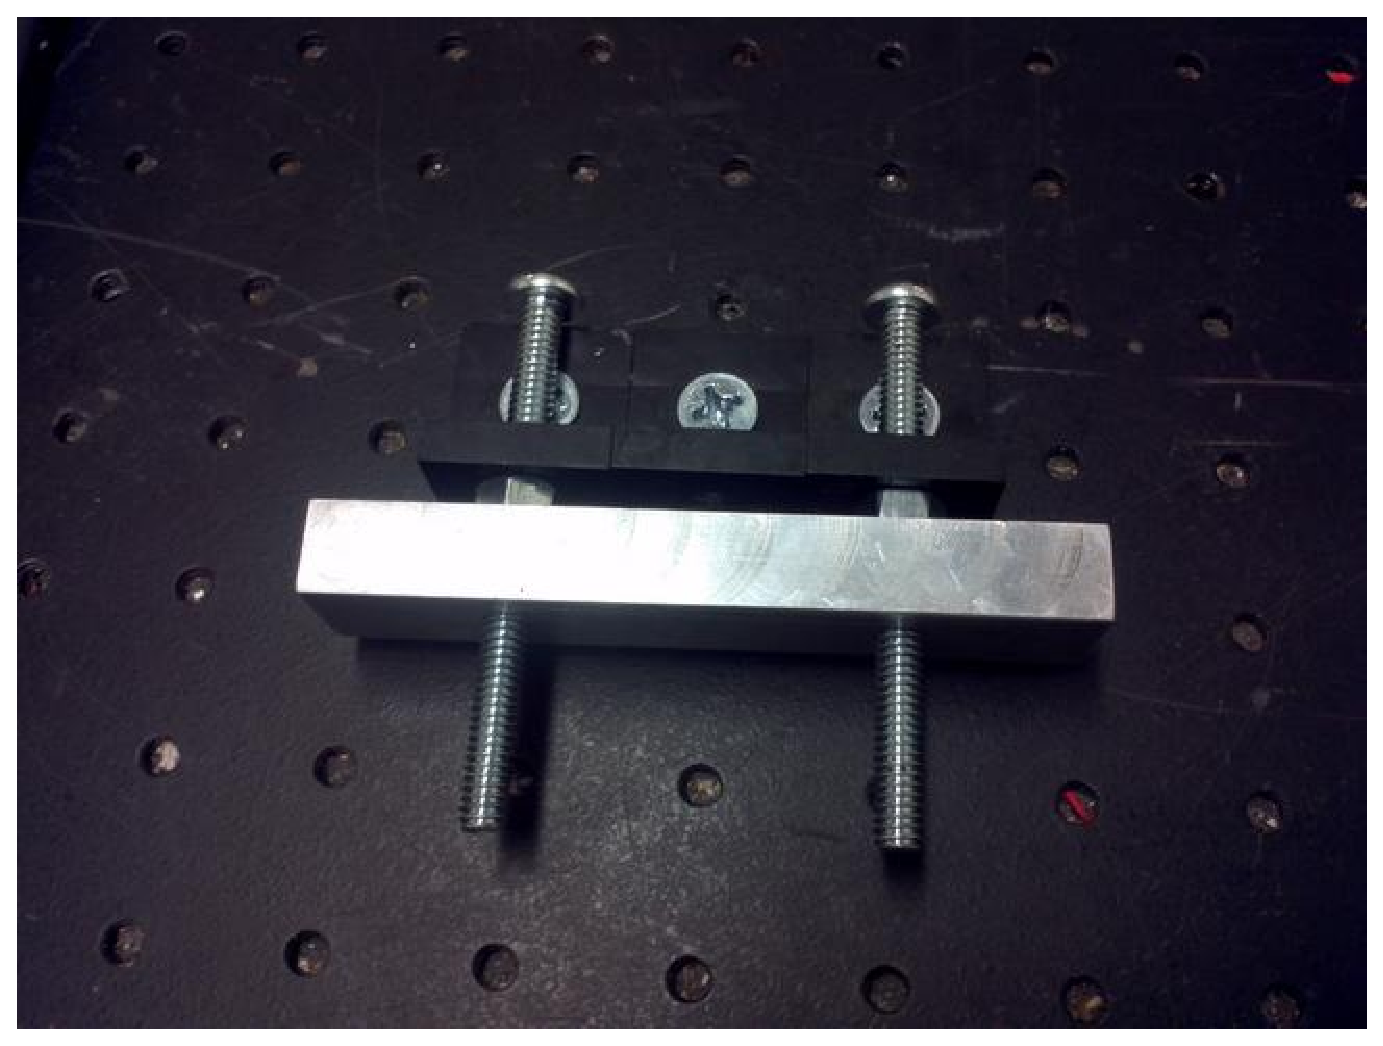
\includegraphics[width=0.7\textwidth]{eps_pics/rsCompression}}
\end{subfigmatrix}

   \caption
%>>>> use \label inside caption to get Fig. number with \ref{}
   { \label{fig:compression}
(a) The left side compression mechanism. The middle bolt was used to adjust the compression in the system by using it to move the aluminum block back and forth;
(b) Right side compression mechanism. This had two nuts to adjust the aluminum bar's positions so it could accommodate different rod sizes.
 }
   \end{figure}

\begin{figure}[ht!]
\centering
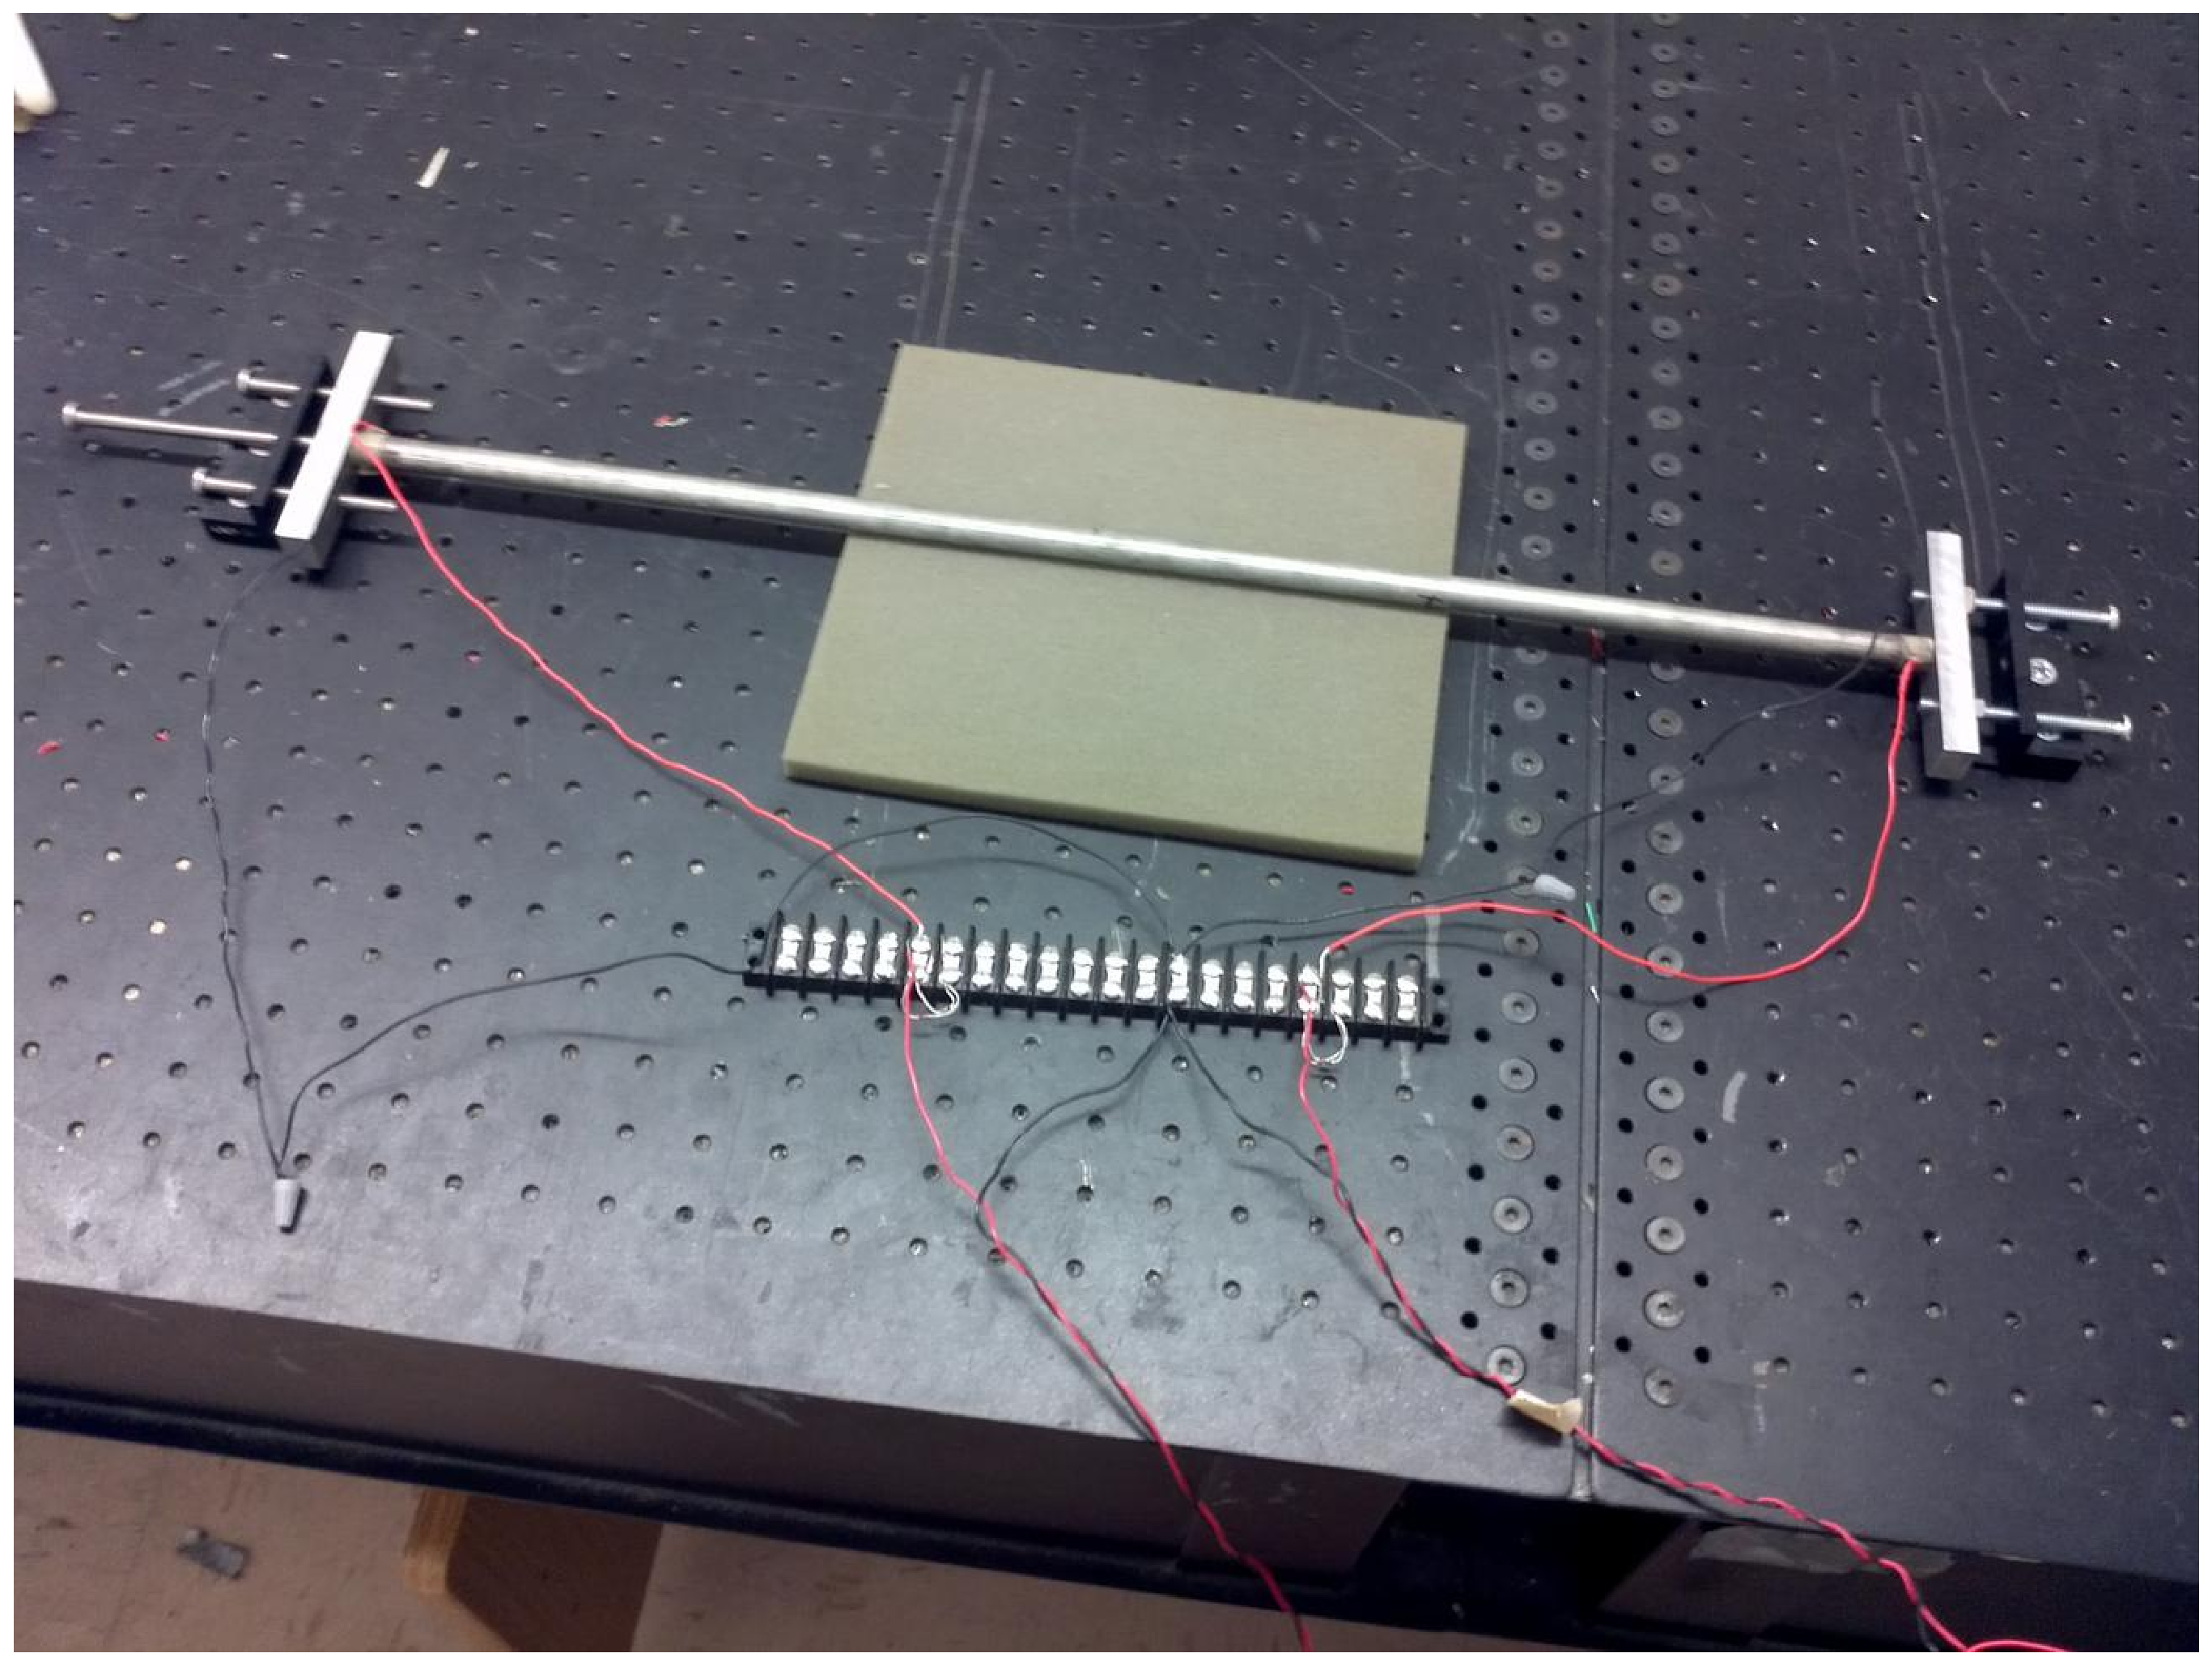
\includegraphics[width=0.7\textwidth]{eps_pics/steelUncrackedFull}
\caption{Steel rod with PZTs affixed to each end using accelerometer putty. The system is in compression using the custom mechanism and is seen on the optics table. The PZT on the left is referred to as PZT A and the right PZT is referred to as PZT B. 
 	 \label{fig:steelUncrackedFull}} 
\end{figure}

\begin{figure}[ht!]
\centering
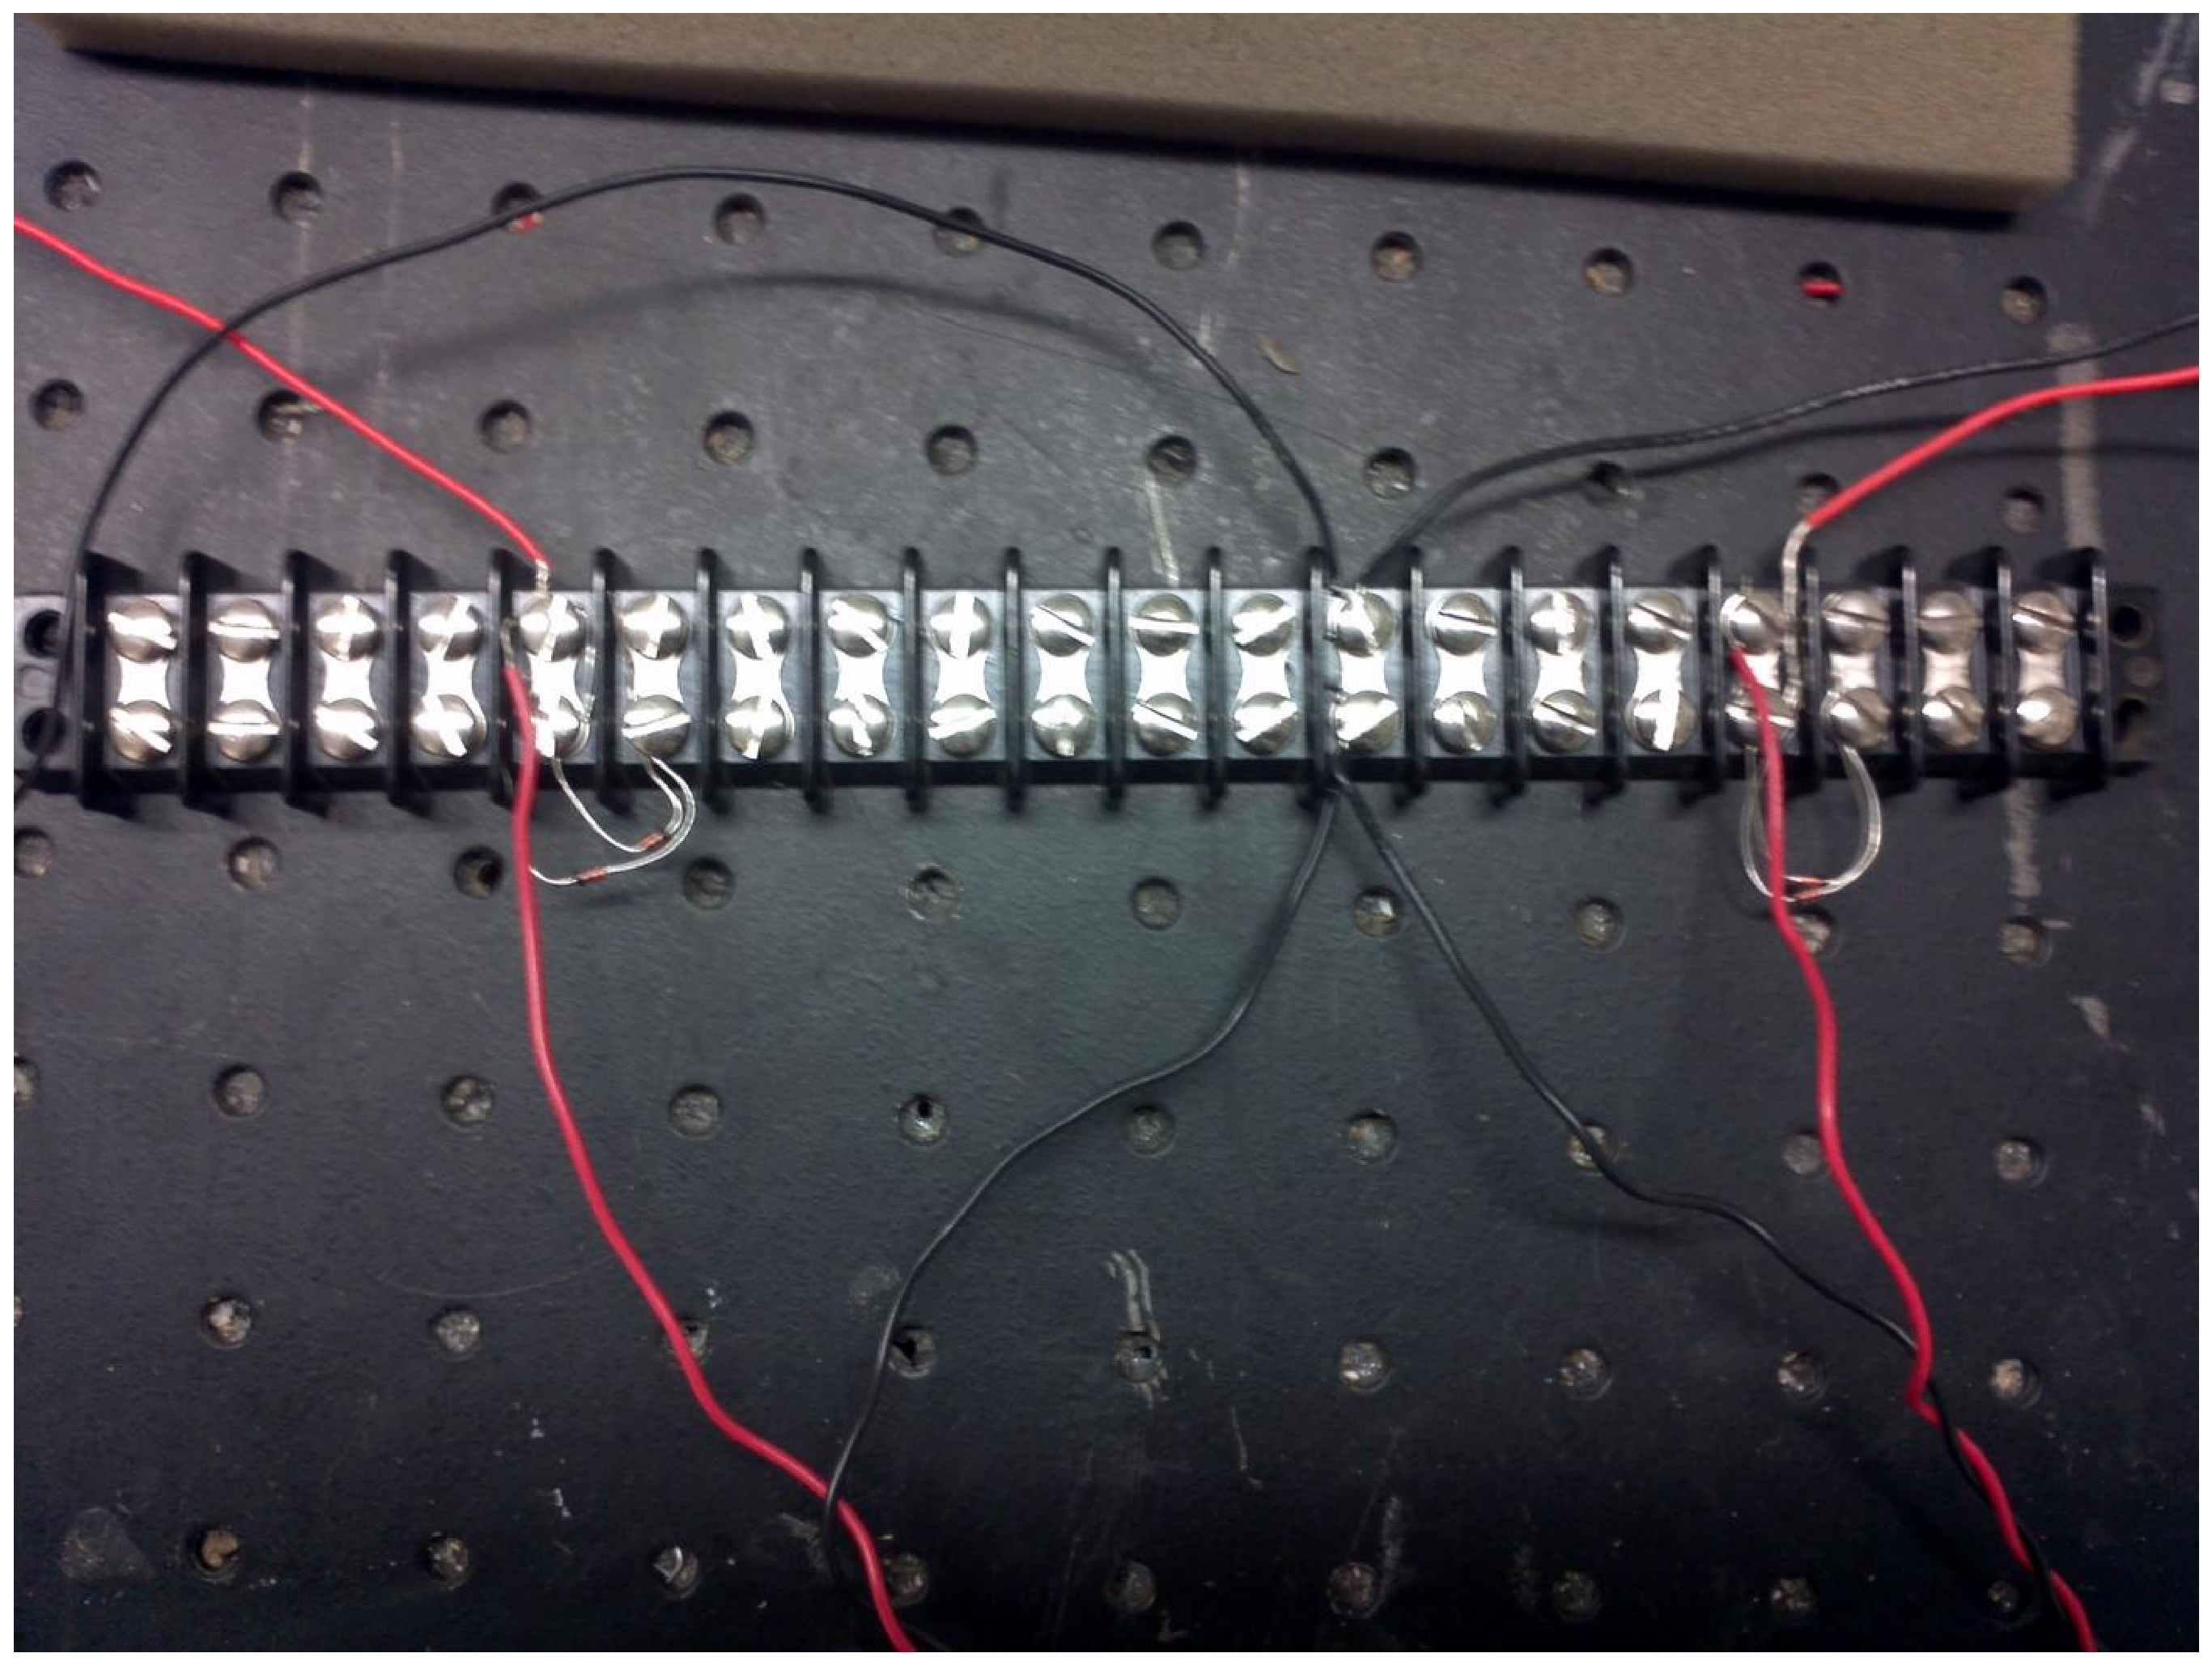
\includegraphics[width=0.7\textwidth]{eps_pics/junctionBox}
\caption{Simple terminal block that was used for handling the connections among the various data acquisition wires. Also contained on the terminal block is a diode circuit between the amplifier output and the analog read in line for each PZT. 
 	 \label{fig:junctionBox}} 
\end{figure}

\begin{figure}[ht!]
\centering
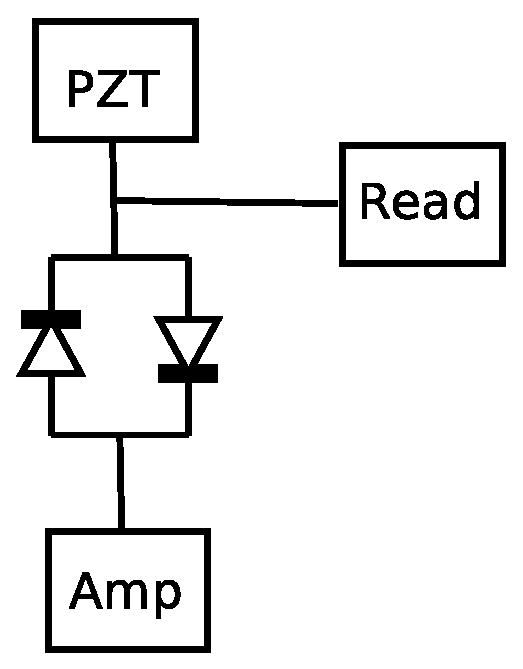
\includegraphics[width=0.3\textwidth]{eps_pics/diodeCircuit}
\caption{Diode circuit that is placed between the amplifier output and analog read in lines for each PZT. This circuit snuffs out the noise produced by the amplifiers at the expense of a slight reduction in voltage output to the PZTs. 
 	 \label{fig:diodeCircuit}} 
\end{figure}

The software used consisted of two main programs which were the host program and the FPGA program. The host program ran on the PC and the FPGA program was downloaded to the FPGA card where it was executed. Communication between the host and FPGA programs was handled with the FPGA's First-In-First-Out memory protocol (FIFO) to which the host program had direct memory access (DMA).The synchronization of the data transactions between the host and FPGA programs is handles using a handshaking protocol implemented by IRQs. 

The purpose of this set of experiments was to determine if the occurrence of a crack could be detected within the steel rod. The idea is to send a signal from PZT A and record the response at PZT B. This continues and successive responses are compared to the first response and the program attempts to detect a significant change between the responses which indicates that something in the medium has changed and potentially represents the appearance of a crack. For the implementation, the host program first generated an initial multi-tone wave. The wave is composed of individual sinusoidal waves of different frequency that were concatenated together to form the overall mutli-tone wave. The center frequency for the multi-tone wave was $115 kHz$ and had a bandwidth of $30 kHz$. The relationship between the number of points needed to create the wave and the sampling frequency of the FPGA card (740.741 kHz here) was used to obtain the correct frequency for each wave. A total of 7,8, and 9 data points were used by the program to represent a single sinusoidal wave period of the $130 kHz$, $115 kHz$, and $100 kHz$ wave components, respectively. The $130kHz$ wave was placed in the center of the wave grouping with a $115kHz$ wave on both sides of it and then a $100 kHz$ wave on the ends of the grouping (Figure \ref{fig:initialWave}). 

\begin{figure}[ht!]
\centering
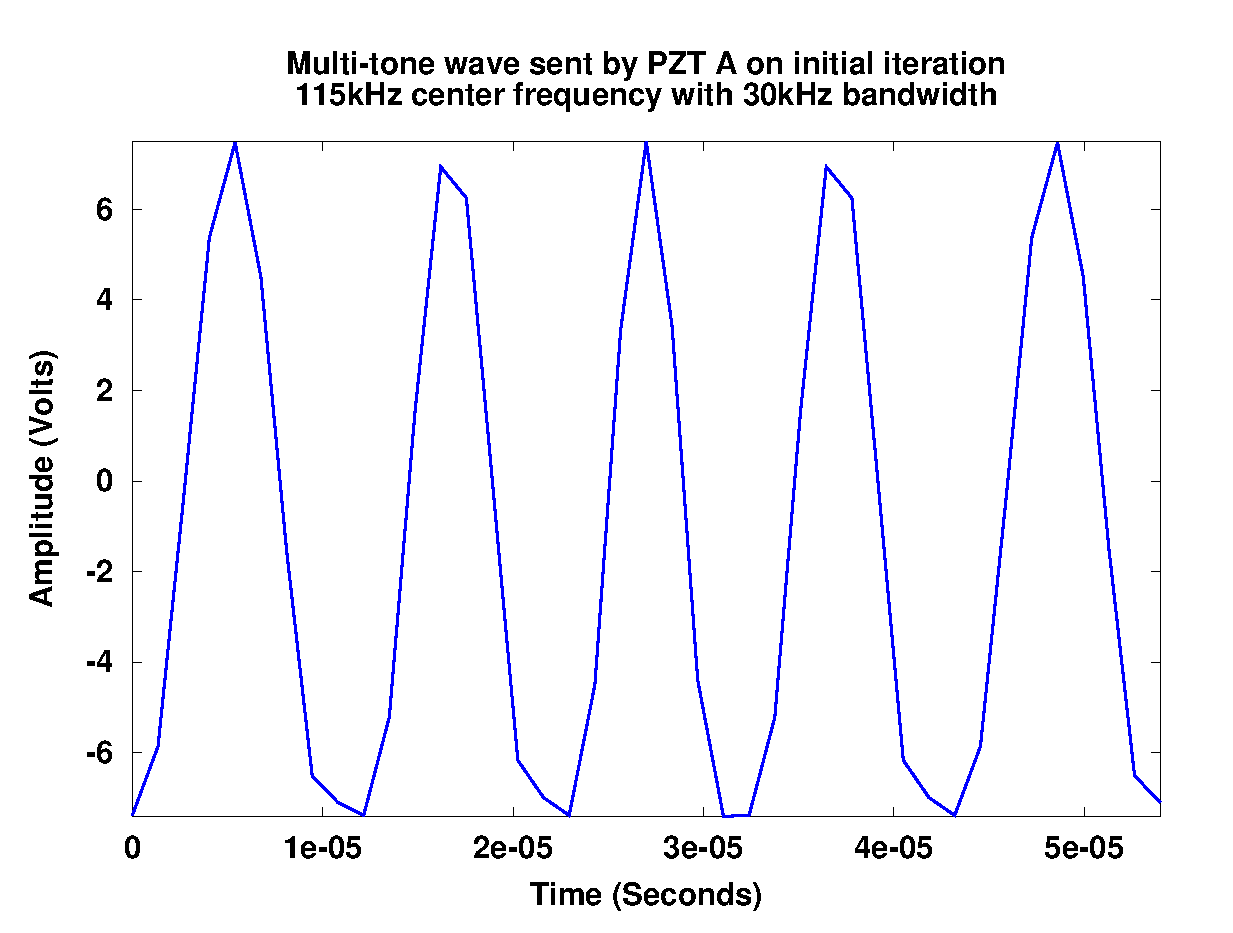
\includegraphics[width=0.6\textwidth]{eps_pics/initialWave}
\caption{Mutli-tone wave that was played out by PZT A. The wave was created by concatenating single period sinusoidal waves of different frequency. The wave in the middle is $130kHz$, the waves next to it are $115kHz$, and the outside waves are $100kHz$. It was found that this multi-tone wave caused a better response in the material versus using a single frequency.
 	 \label{fig:initialWave}} 
\end{figure}

After the wave was generated it was transferred to the FPGA program which then zeroed all of its output values and waited for $200ms$. This wait time was chosen based upon experimental results for the time of a signal to decay when propagating through a steel or nylon rod. Once the wait time elapsed, the signal was sent into the rod by PZT A. The wave propagated through the rod and was recorded on the other end by PZT B. This was performed five times total and the response for each iteration was recorded. With the data for the undamaged rod recorded it was time to test a damaged sample. The damaged steel rod was created  by taking the undamaged rod that was used and cutting it in to two pieces of arbitrary length (Figure \ref{fig:steelPieces}). A PZT was placed on one end of each piece and the free ends of the pieces were pressed together. What was formed was essentially the same rod that was previously but with a crack location at an arbitrary position (Figure \ref{fig:steelCrack}). The program was then ran five times on the new setup with a signal being sent by PZT A and recorded at PZT B.

\begin{figure}[ht!]
\centering
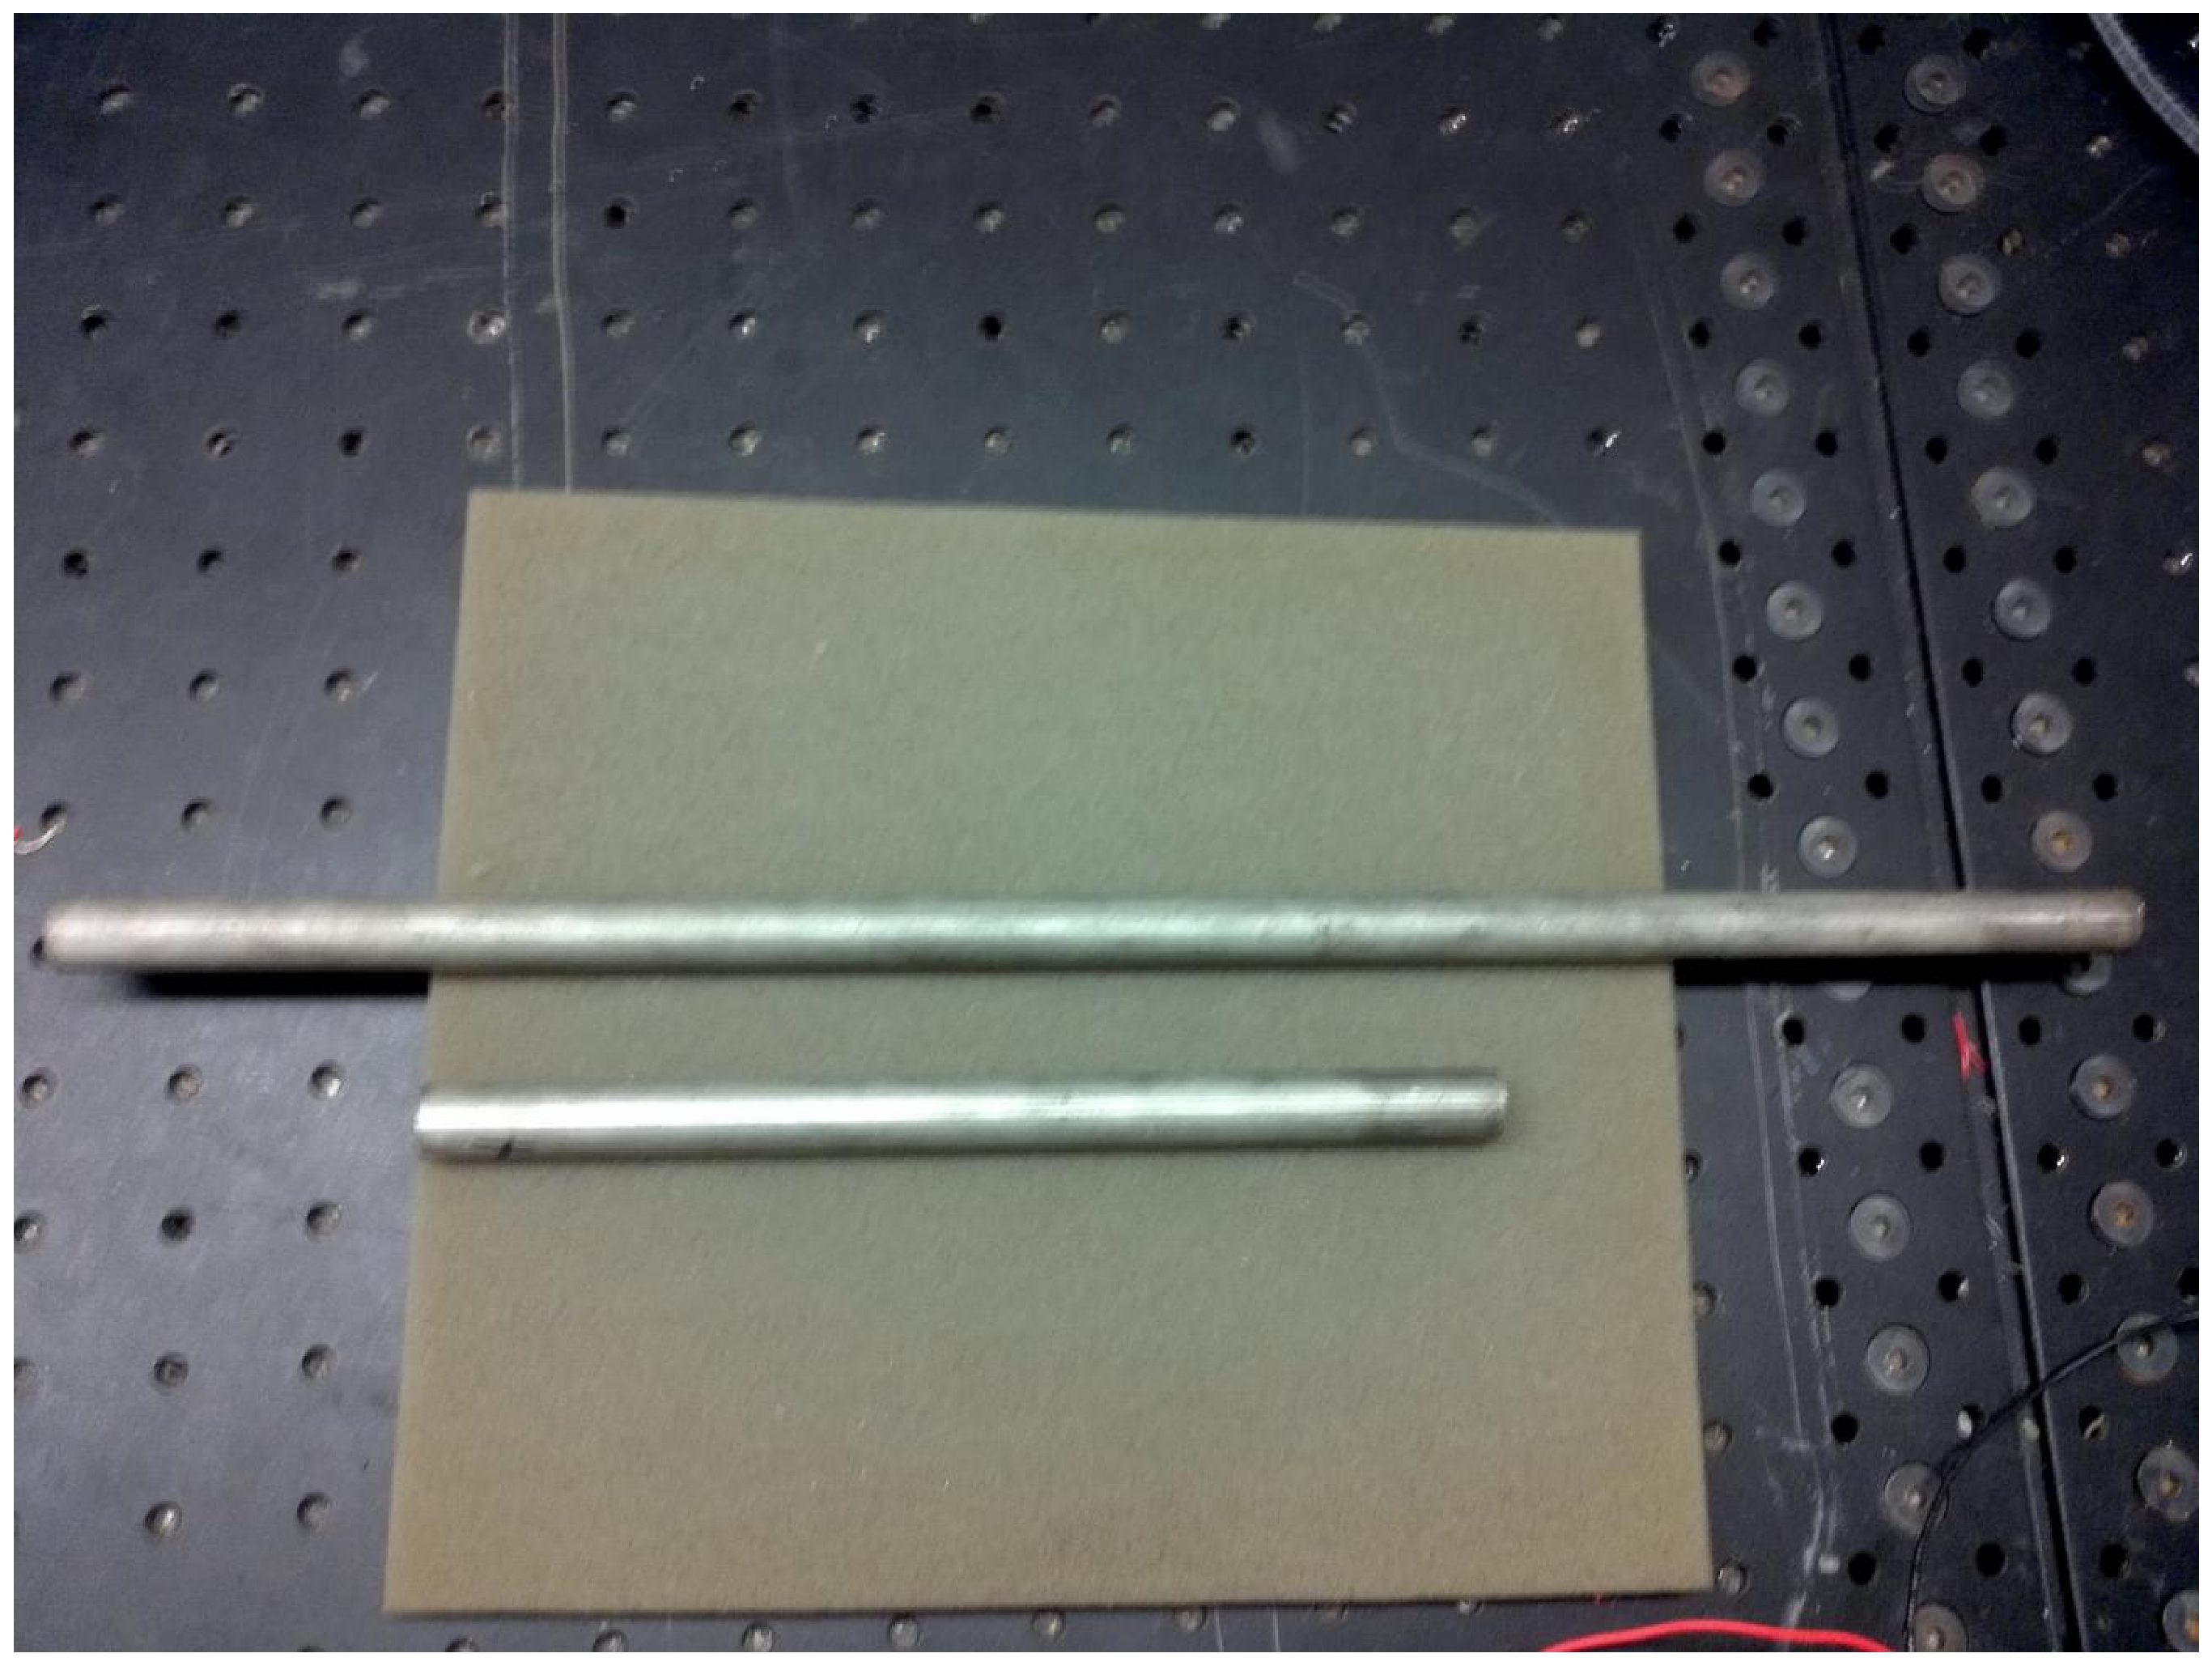
\includegraphics[width=0.6\textwidth]{eps_pics/steelPieces}
\caption{Undamaged rod that has been cut in to two pieces of random length. This pieces are then pushed together (end to end) to represent a rod with a crack location.
 	 \label{fig:steelPieces}} 
\end{figure}

\begin{figure}
\begin{subfigmatrix}{2}
\subfigure[Full view of steel 'damaged rod' tests]
{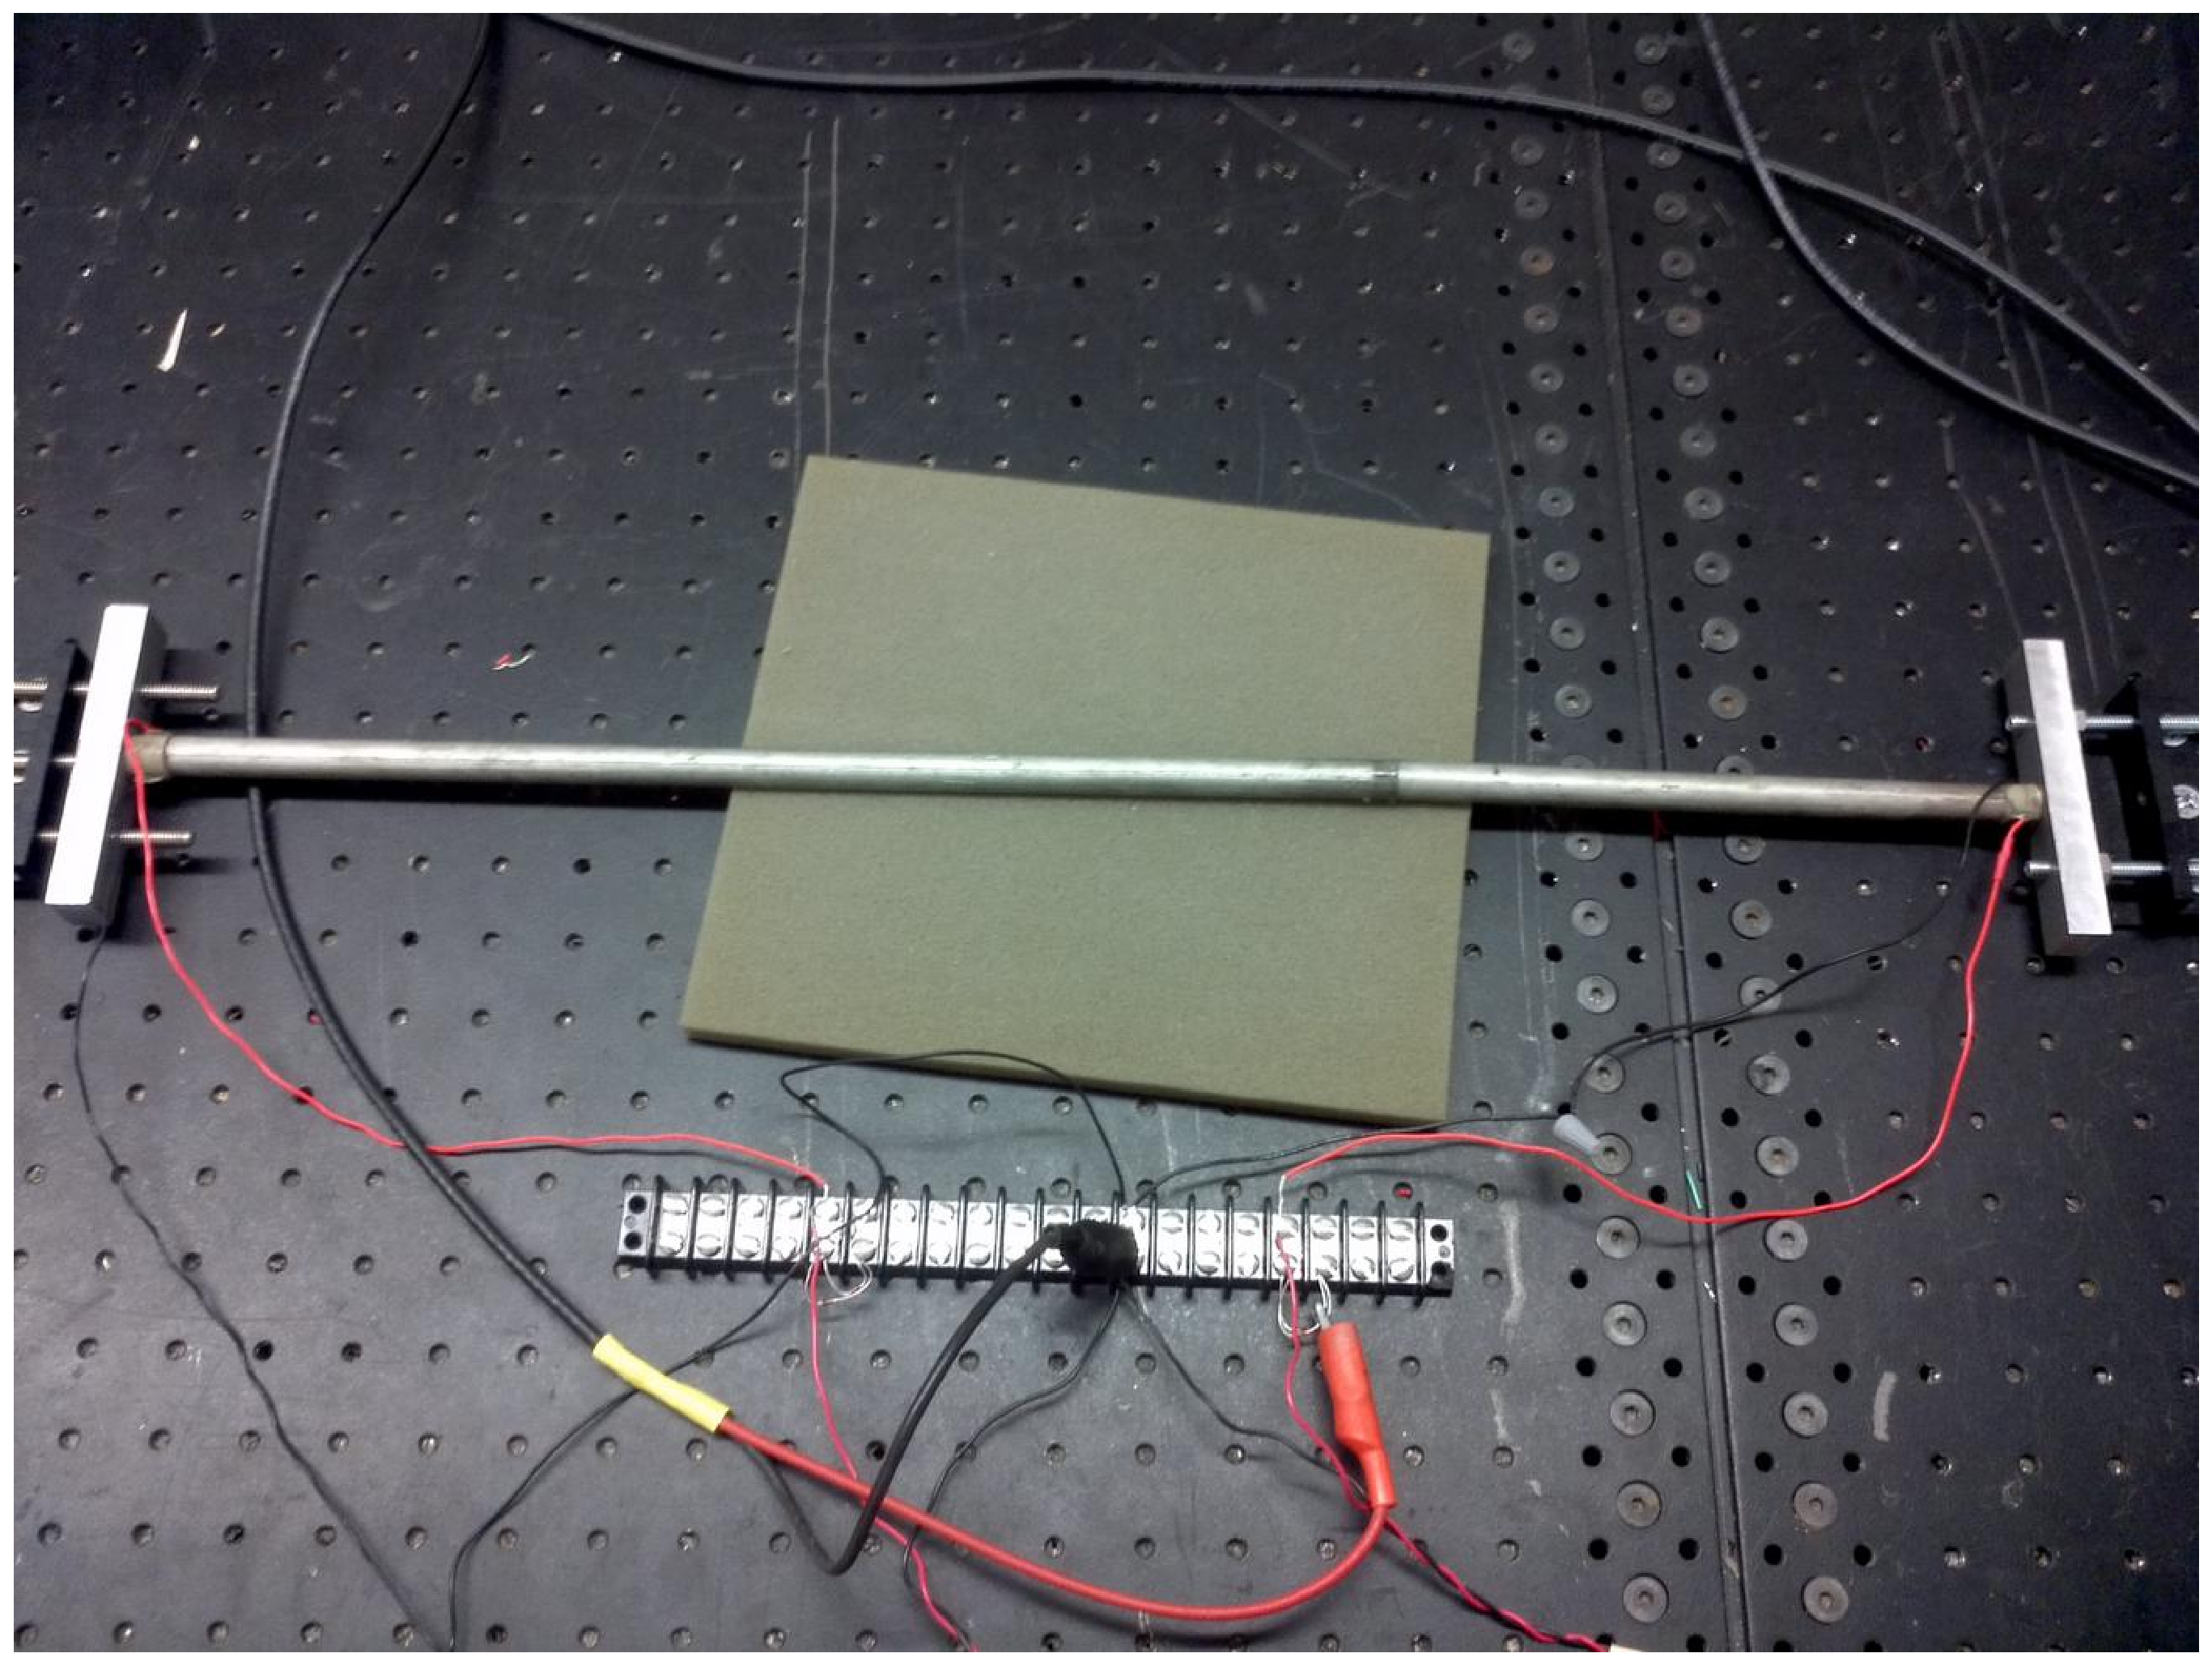
\includegraphics[width=0.6\textwidth]{eps_pics/steelCrackFull}}
\subfigure[Close up of the defect location ]
{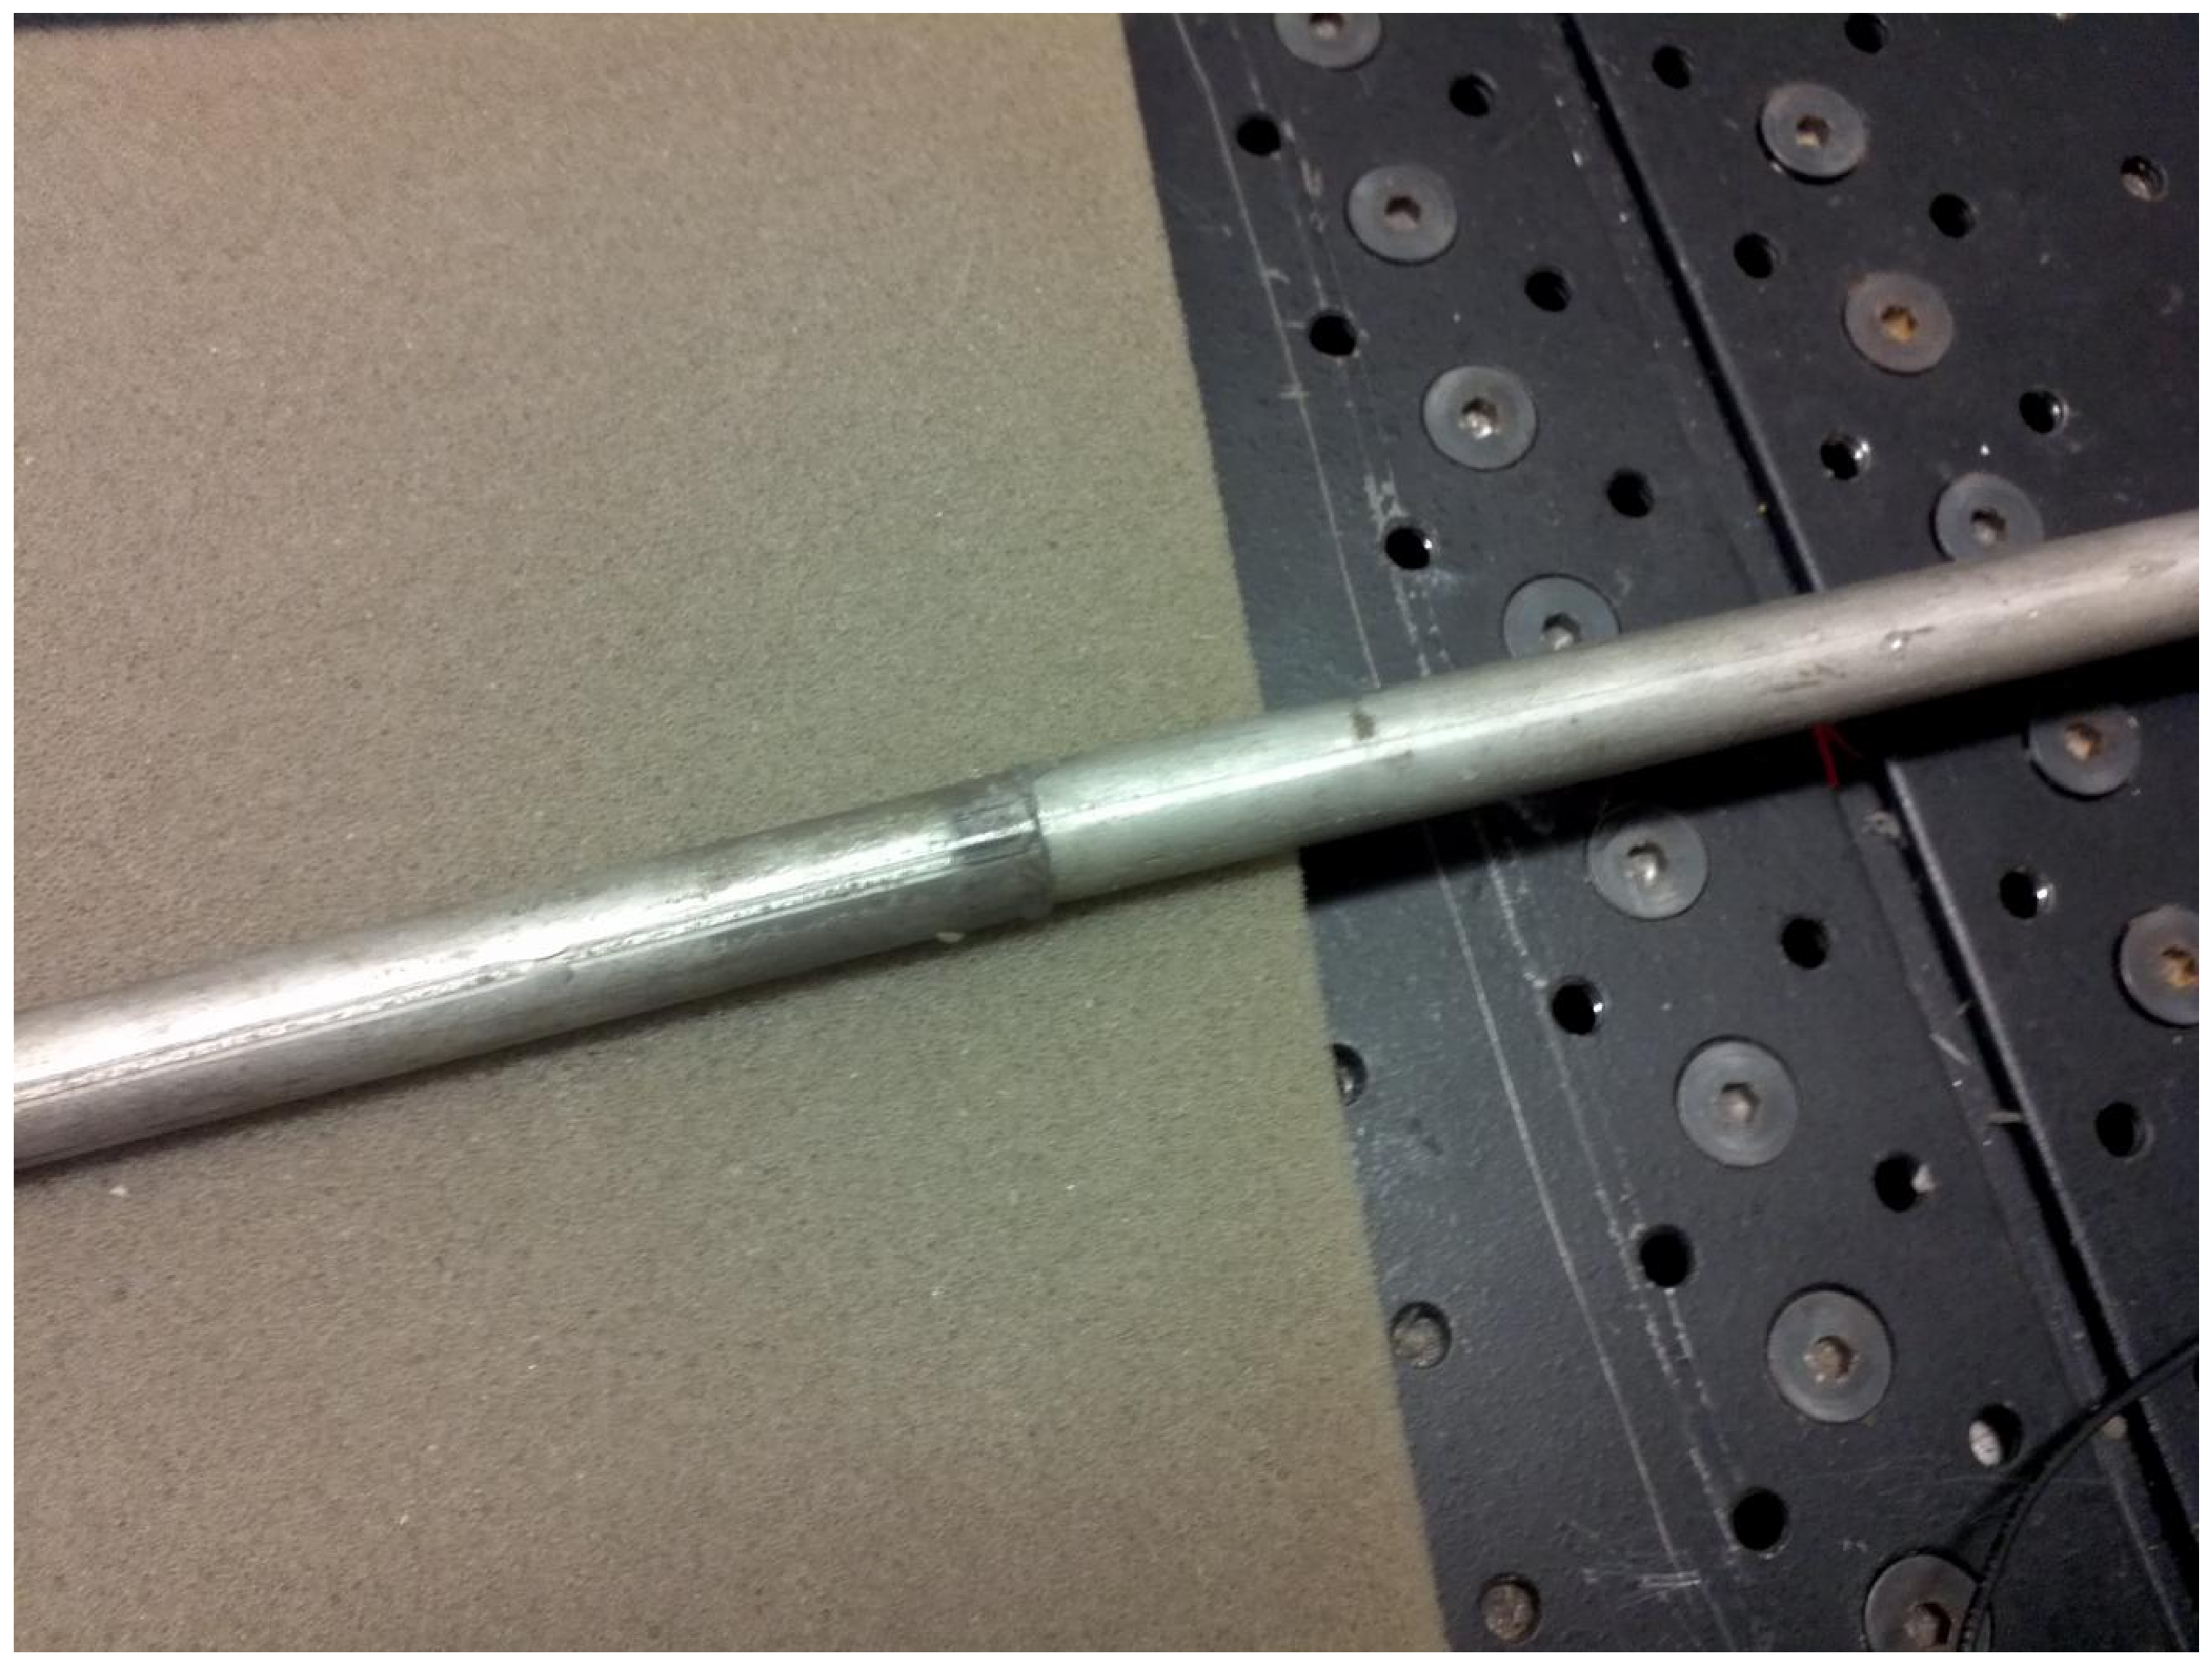
\includegraphics[width=0.6\textwidth]{eps_pics/steelCrackClose}}
\end{subfigmatrix}

   \caption
%>>>> use \label inside caption to get Fig. number with \ref{}
   { \label{fig:steelCrack}
(a) Full view of the two steel rod pieces that are pressed together to represent a rod with a defect location.;
(b) Close up view of the defect location in the steel rod system which should cause a noticeable change in the response at PZT B.
 }
   \end{figure}
   
A MATLAB program read in the data from each run and compared the responses using a simple sum of differences squared formula. The five signals for each test were also averaged together to get a better idea of what the signal looks like in the undamaged tests compared to the damaged rod tests.

These exact same tests were then carried out for a nylon rod. The nylon rod was found to have a density of $0.854 \times 10^3 kg/m^3$, an elastic constant of $4.68121 \times 10^9$ and a length of $148 \times 10^{-3} m$. The setup for the nylon rod tests is shown in Figures \ref{fig:nylonUncrackedFull} and \ref{fig:nylonCrack}.


\begin{figure}[ht!]
\centering
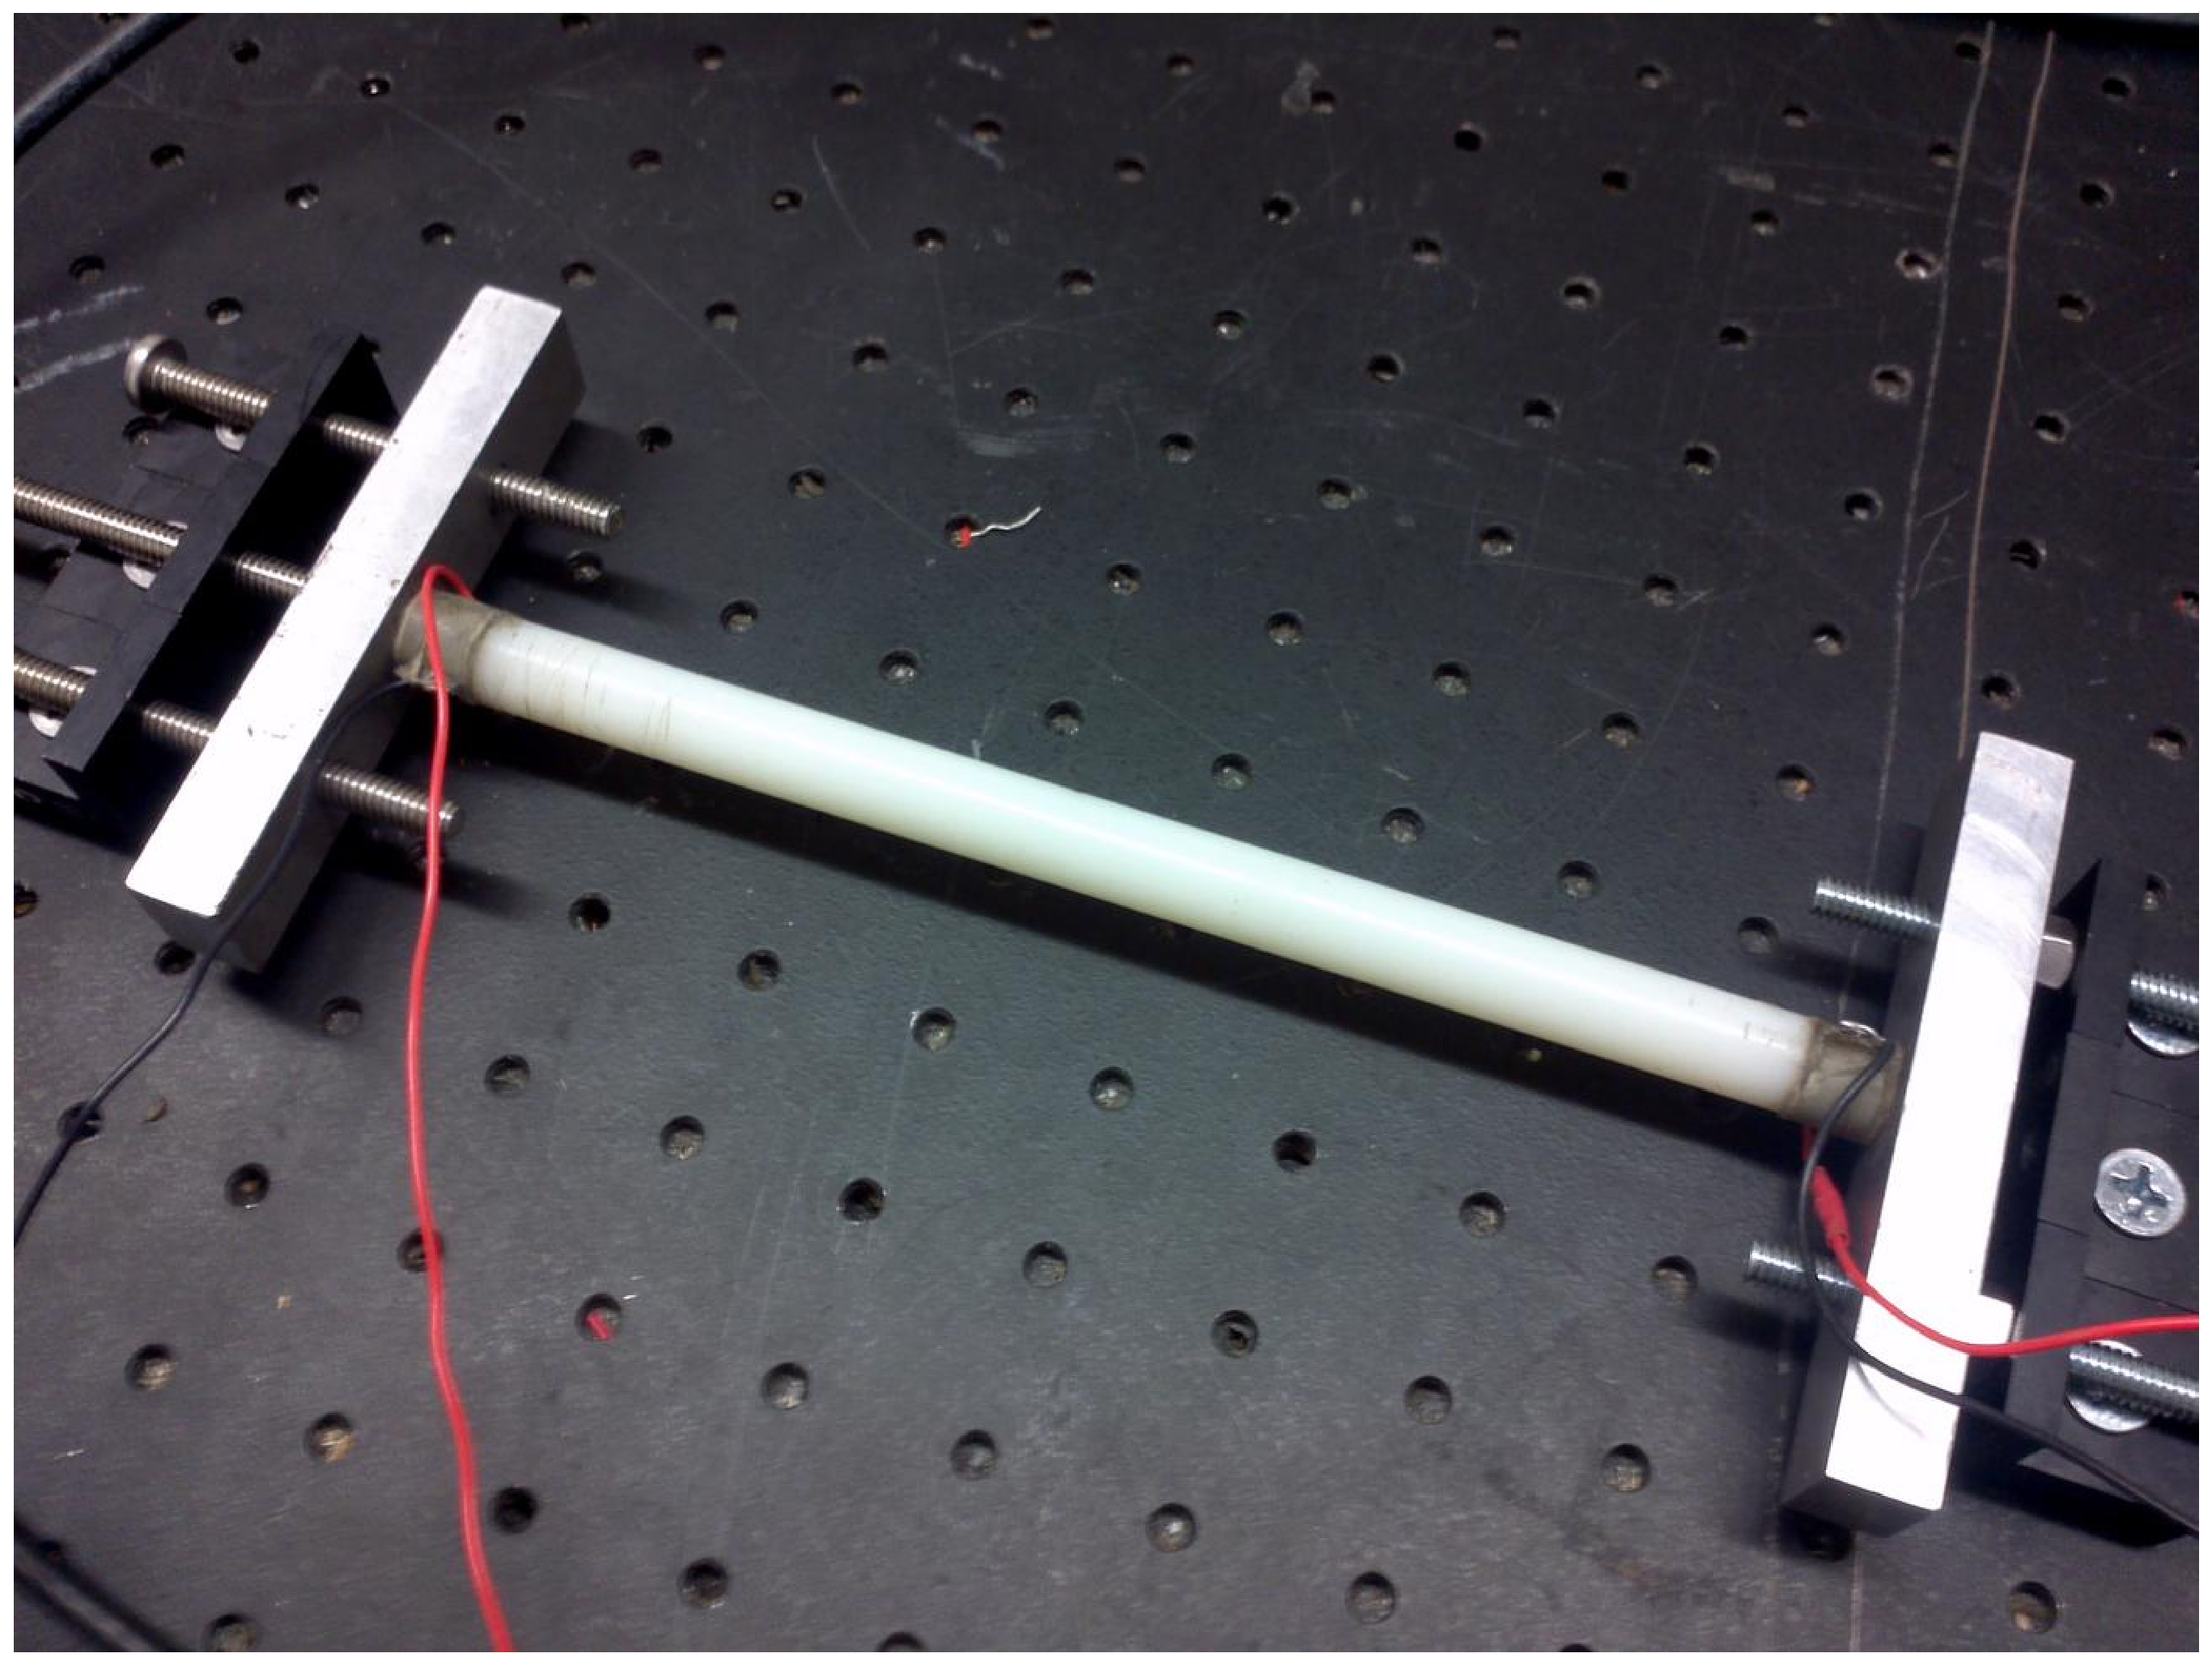
\includegraphics[width=0.6\textwidth]{eps_pics/nylonUncrackedFull}
\caption{Undamaged nylon rod that is setup for testing. A PZT was affixed to each rod end using accelerometer putty and placed into compression using the custom mechanism.
 	 \label{fig:nylonUncrackedFull}} 
\end{figure}

\begin{figure}
\begin{subfigmatrix}{2}
\subfigure[Full view of nylon 'damaged rod' tests]
{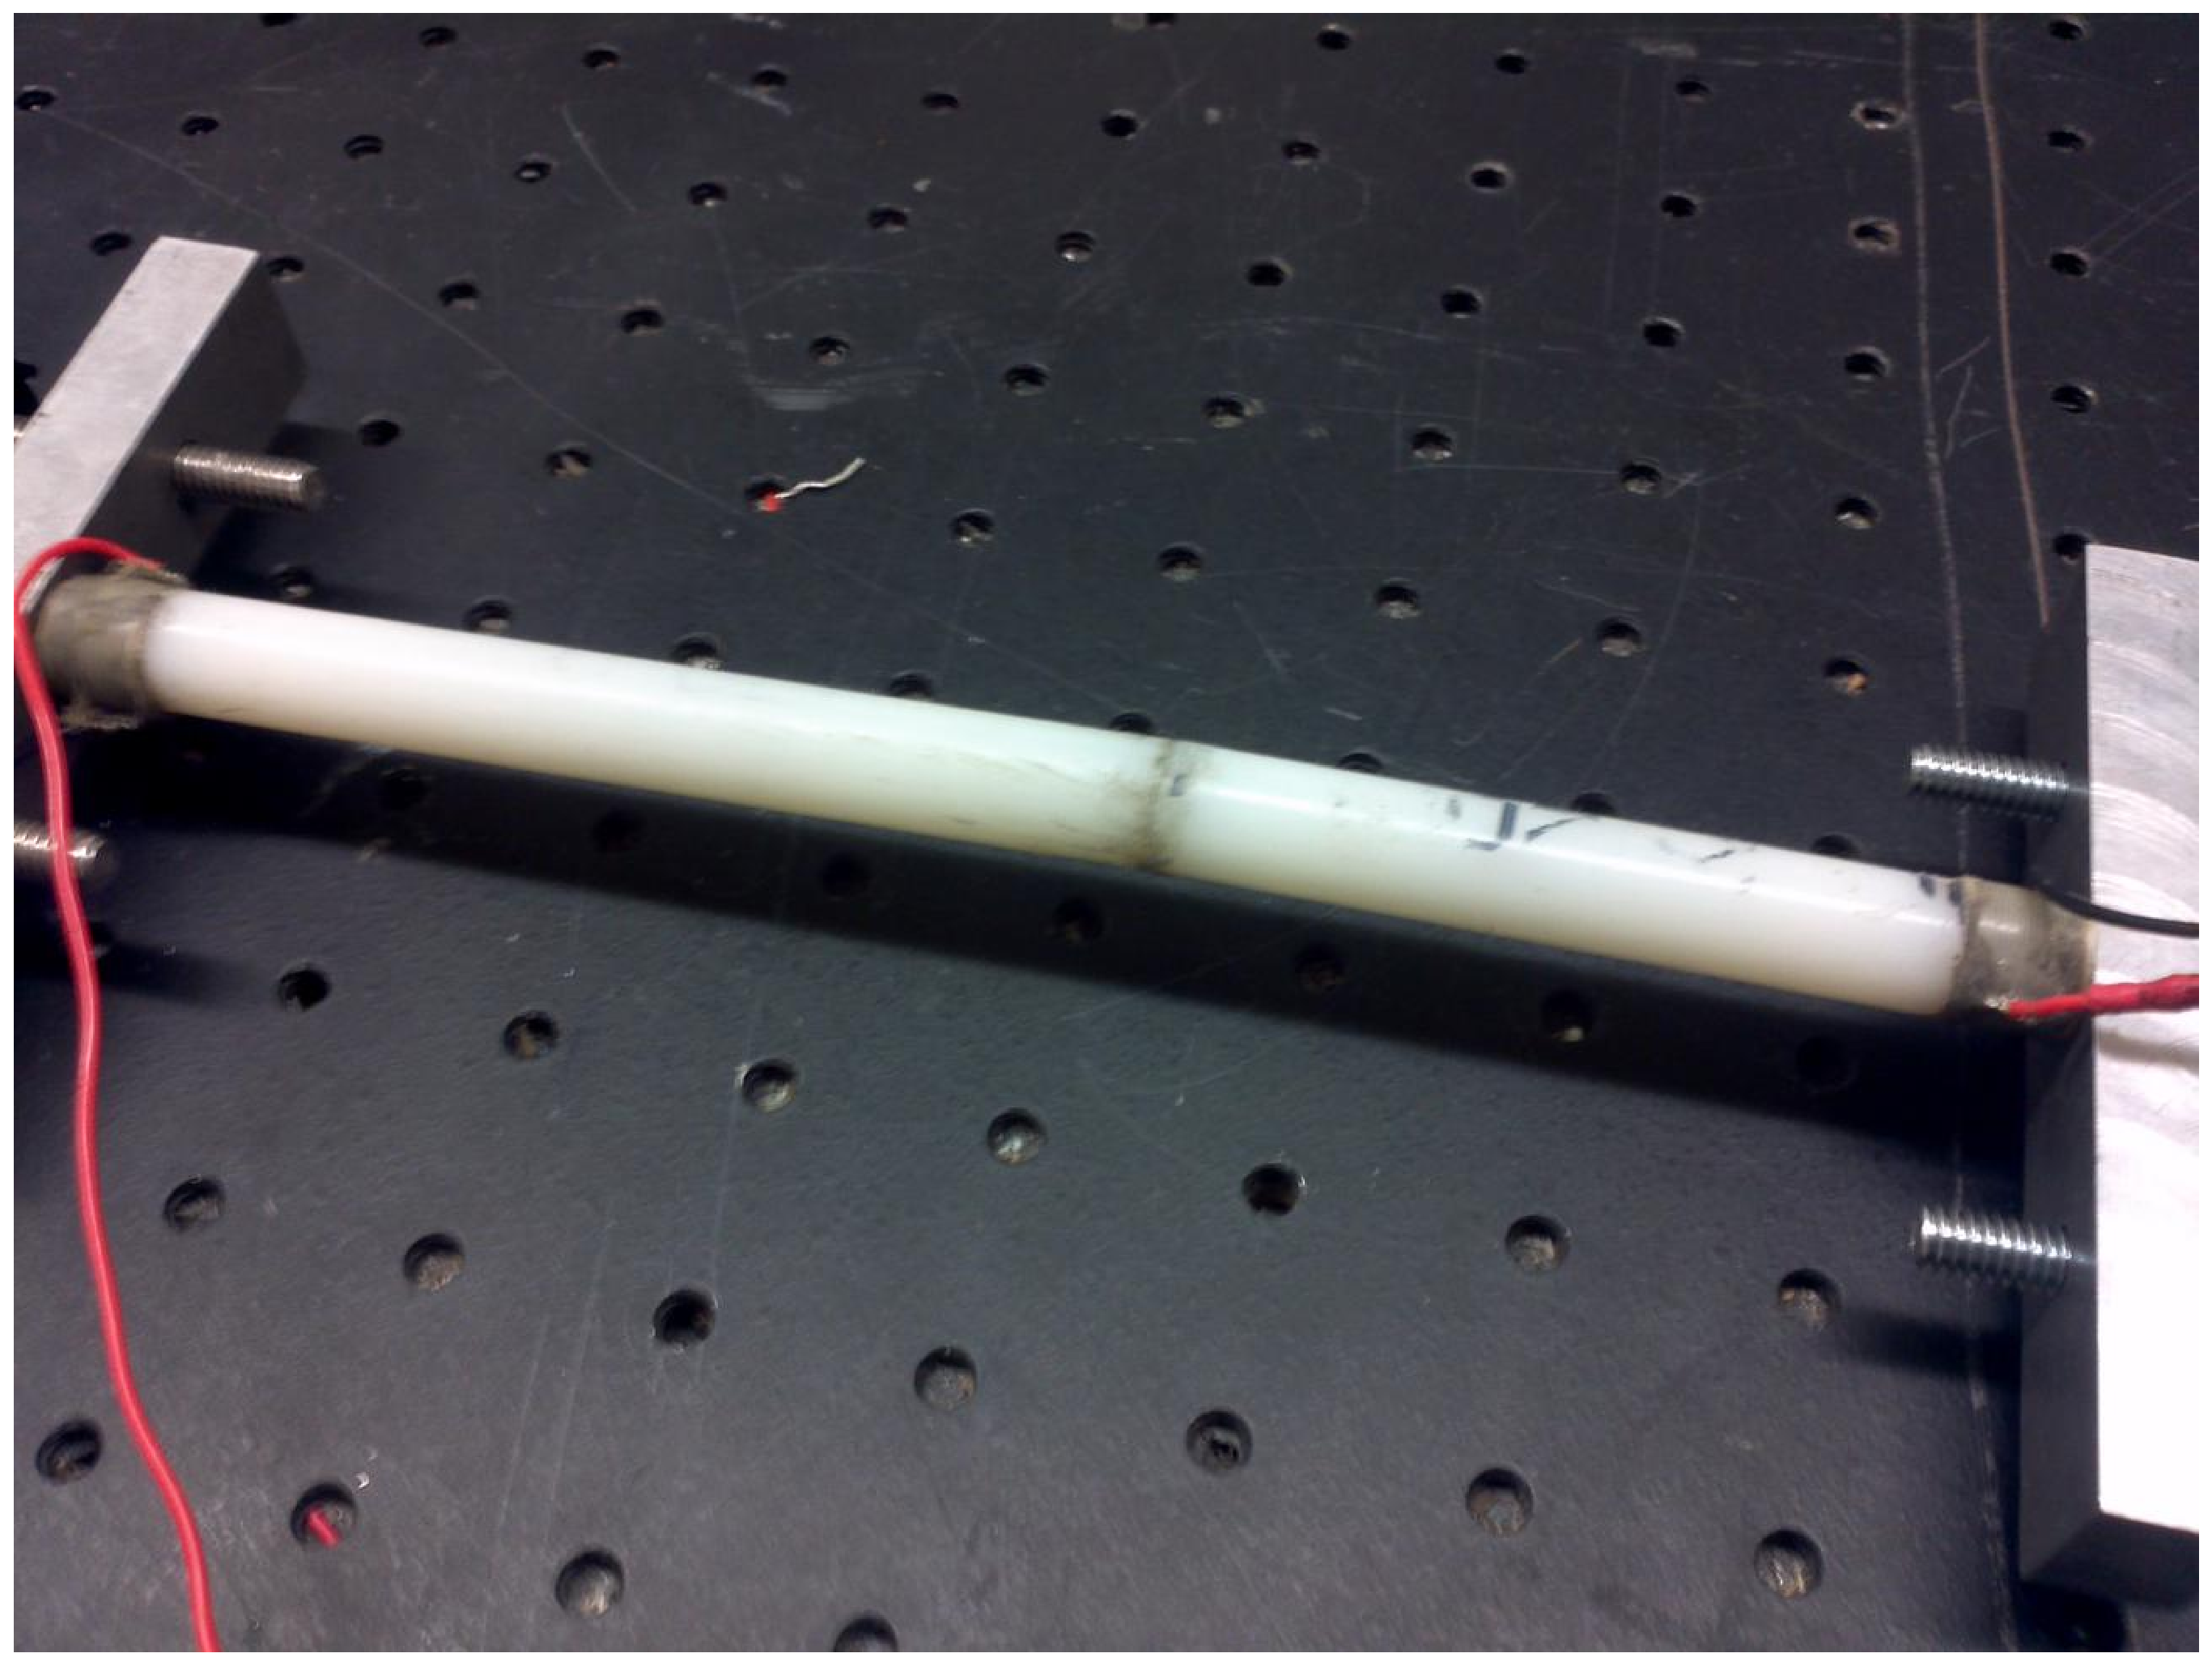
\includegraphics[width=0.6\textwidth]{eps_pics/nylonCrackFull}}
\subfigure[Close up of the defect location ]
{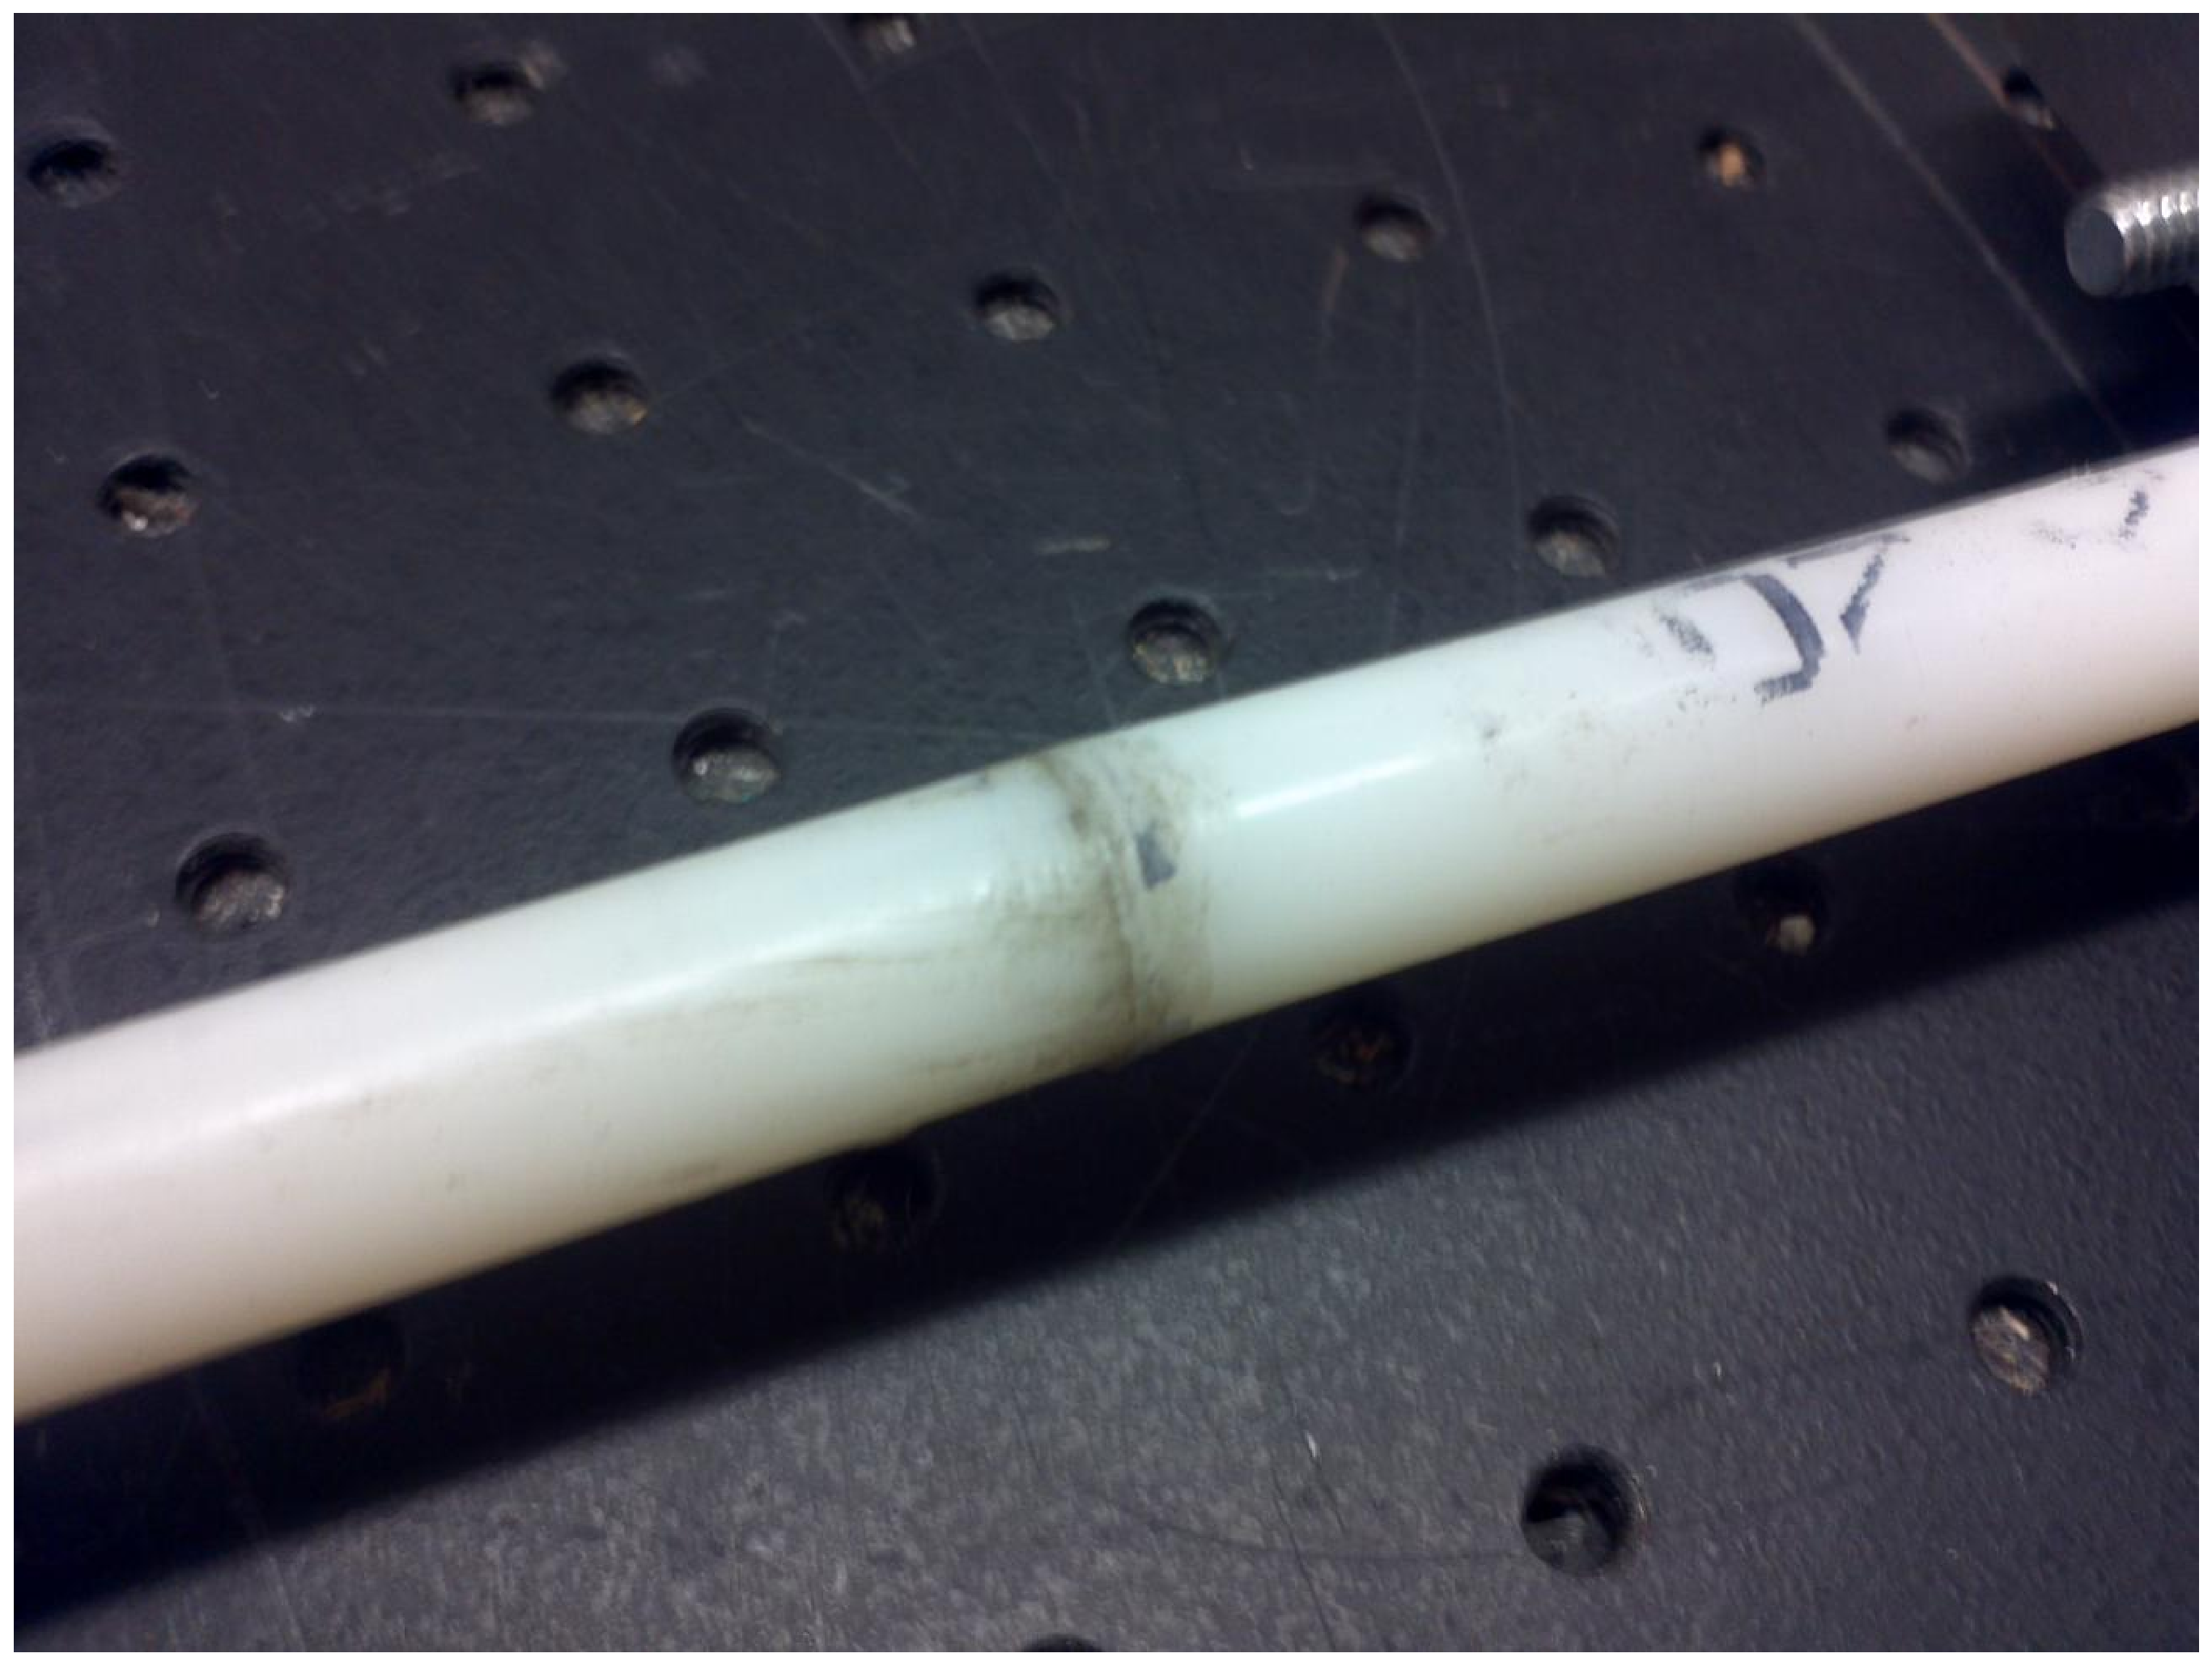
\includegraphics[width=0.6\textwidth]{eps_pics/nylonCrackClose.eps}}
\end{subfigmatrix}

   \caption
%>>>> use \label inside caption to get Fig. number with \ref{}
   { \label{fig:nylonCrack}
(a) Full view of the two nylon rod pieces that are pressed together to represent a rod with a defect location.;
(b) Close up view of the defect location in the nylon rod system which should cause a noticeable change in the response at PZT B.
 }
   \end{figure}
   
\section{Time Reversal Tests}
The next step was to perform acoustic focusing at a crack located at an a priori unknown location. The tests were performed on both steel and nylon rods. The setup was very similar to that described for the crack detection tests. The main difference between these setups is that for the time reversal testing an additional PZT was placed between the two rod sections and will be referred to as the 'defect PZT'. The defect PZT acted as a defect and also provided a way to recorded the response at that location so that the overall effectiveness of the focusing algorithm could be determined. For the steel rod tests, combinations of three rod sections of different length were used which gave a total of three test combinations. The lengths of the steel rods were $579.0 \times 10^{-3} m$, $437.0 \times 10^{-3} m$, and $428.0 \times 10^{-3} m$. Similarly for the nylon rods three lengths were used which were $148.0 \times 10^{-3} m$, $105.0 \times 10^{-3} m$, and $75.0 \times 10^{-3} m$. The setup is shown schematically in Figure \ref{fig:tr_dimensions} and pictorially in Figures \ref{fig:steelTR} and \ref{fig:nylonTR}.

\begin{figure}[ht!]
\centering
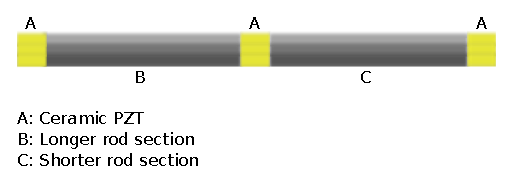
\includegraphics[width=0.8\textwidth]{eps_pics/tr_dimensions}
\caption{Schematic view of the time reversal setup. The PZTs had a length of ~$12.0 \times 10^{-3}m$. The middle PZT is referred to as the defect PZT. The two rod sections used in the tests were of different length and for generality this is just noted as 'longer' and 'shorter' section in the diagram. For the steel rods, the three lengths used were $579.0 \times 10^{-3} m$, $437.0 \times 10^{-3} m$, and $428.0 \times 10^{-3} m$ which gave a total of three combinations ($579.0 \times 10^{-3} m$ and $437.0 \times 10^{-3} m$, $579.0 \times 10^{-3} m$ and $428.0 \times 10^{-3} m$), $437.0 \times 10^{-3} m$ and $528.0 \times 10^{-3} m$). The lengths of the nylon rods used were $148.0 \times 10^{-3} m$, $105.0 \times 10^{-3} m$, and $75.0 \times 10^{-3} m$. The lengths were chosen at random and were unknown to the program during testing.
 	 \label{fig:tr_dimensions}} 
\end{figure}

\begin{figure}
\begin{subfigmatrix}{2}
\subfigure[Full view of steel rod time reversal tests]
{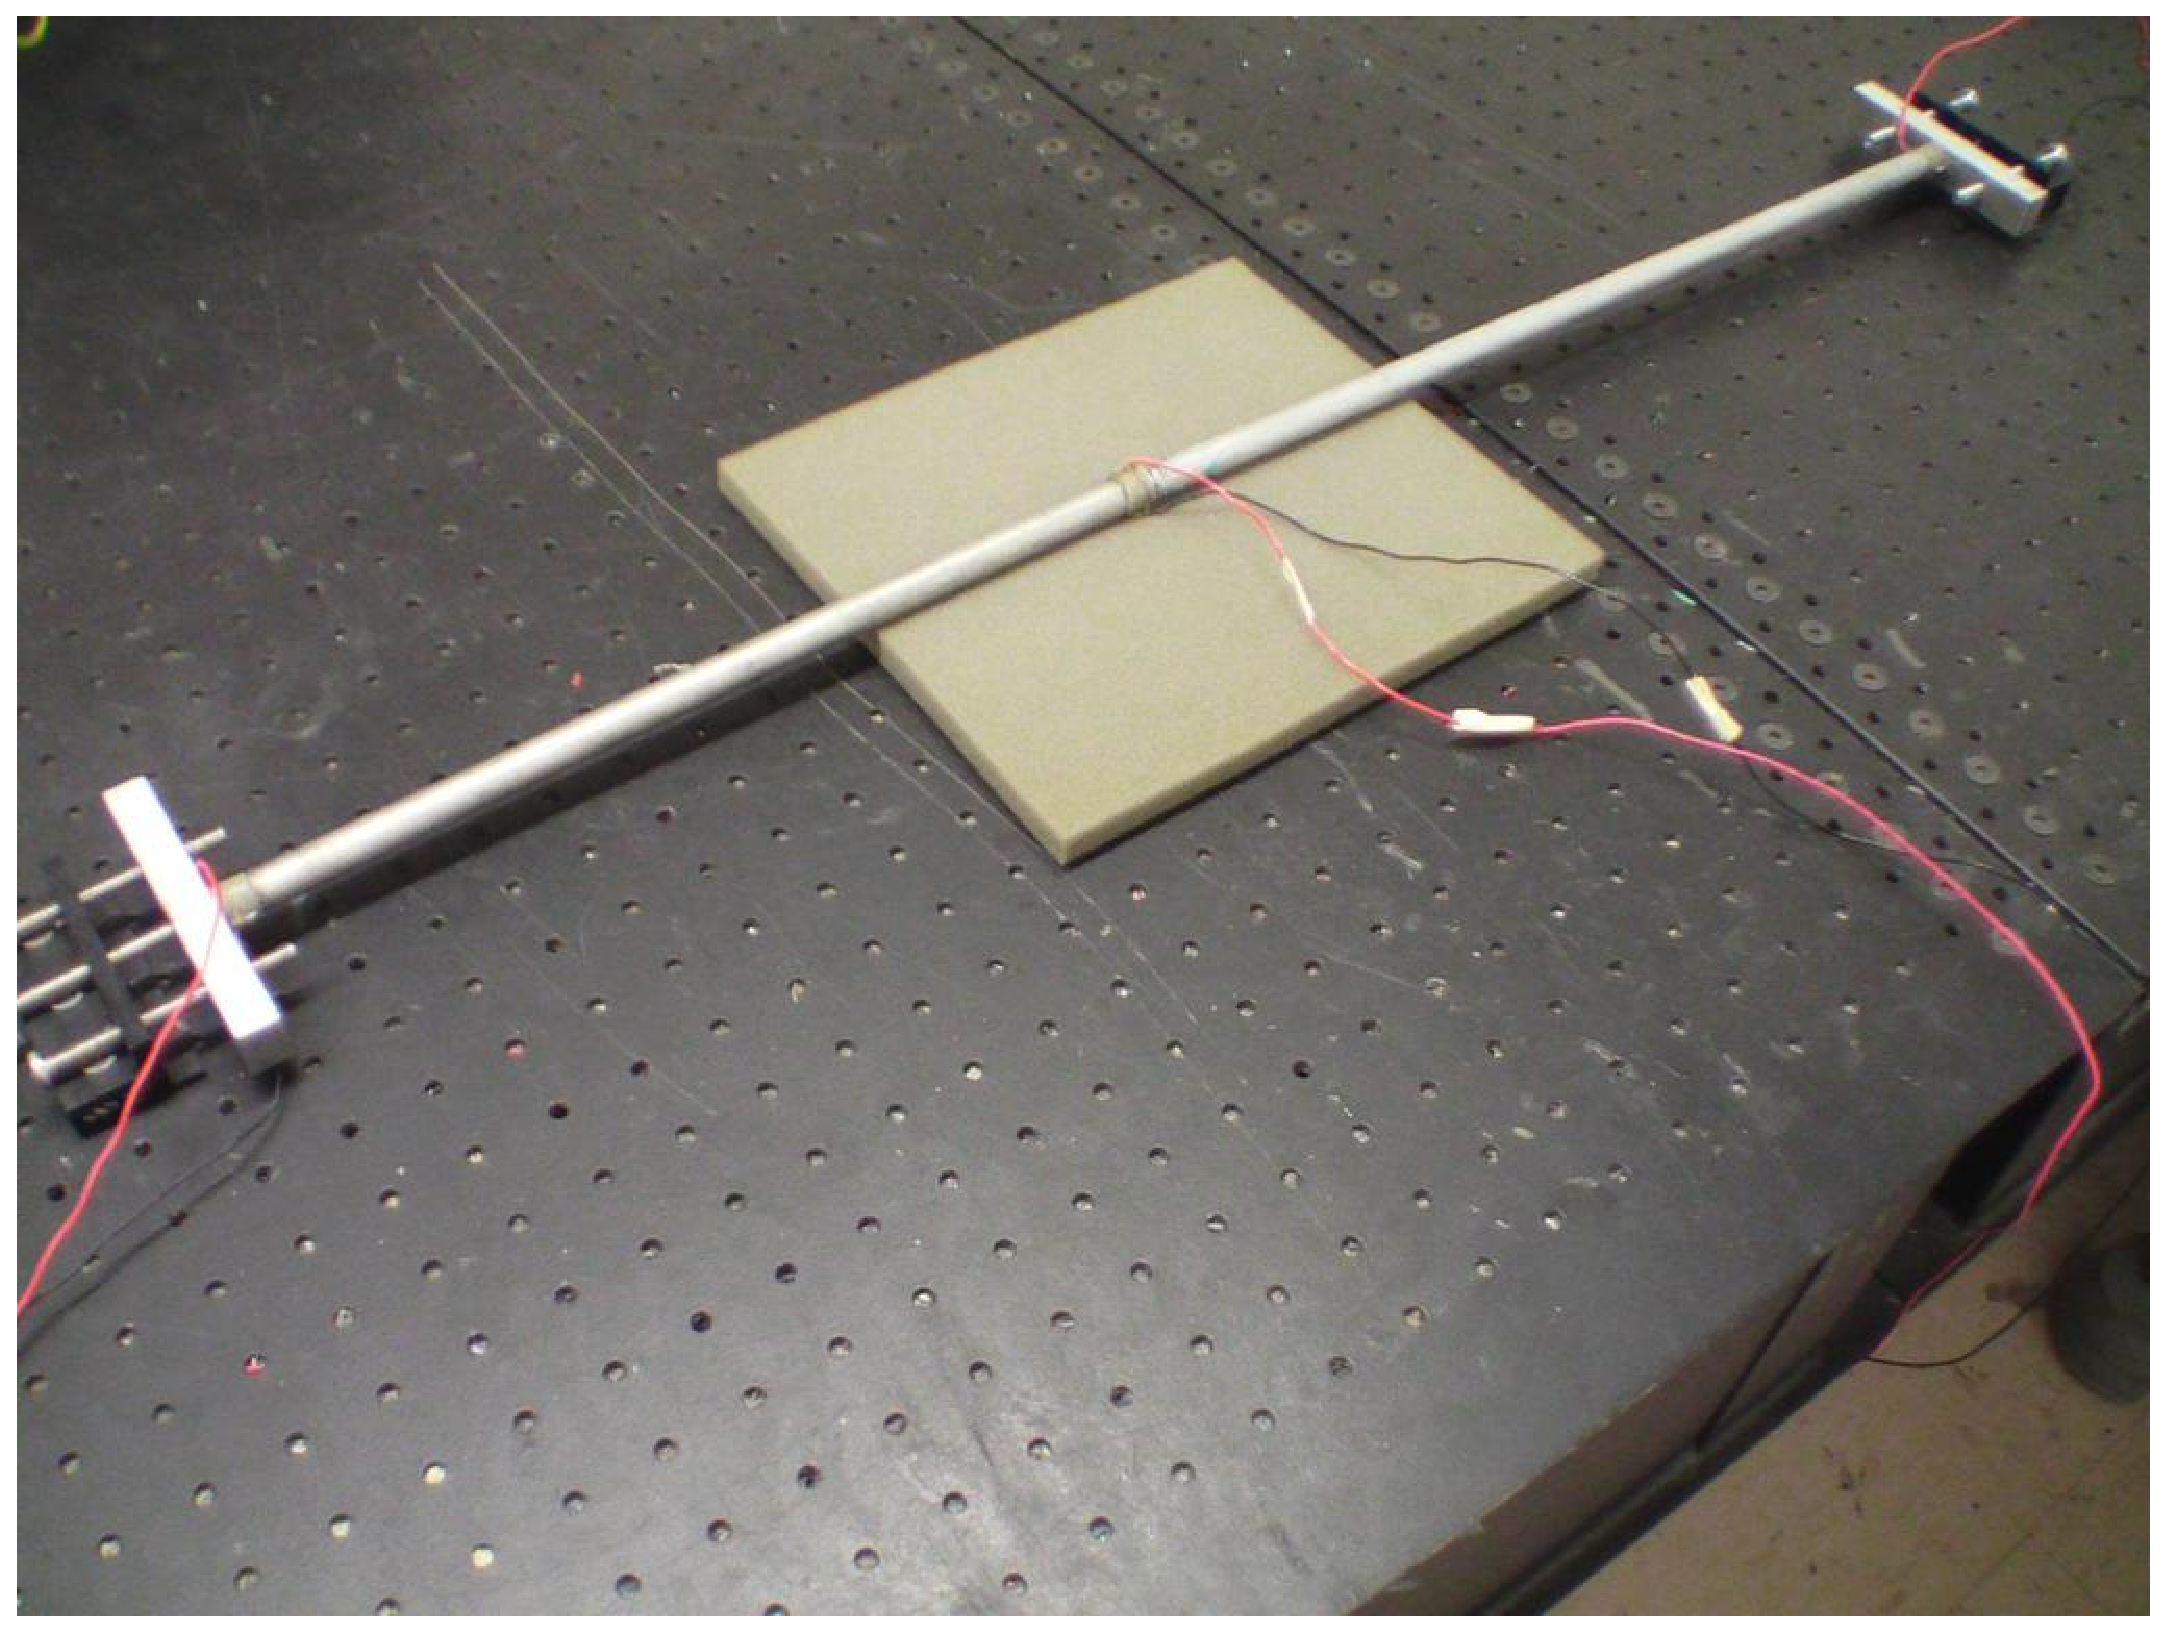
\includegraphics[width=0.6\textwidth]{eps_pics/steelSetupFull}}
\subfigure[Close up of steel rod time reversal tests]
{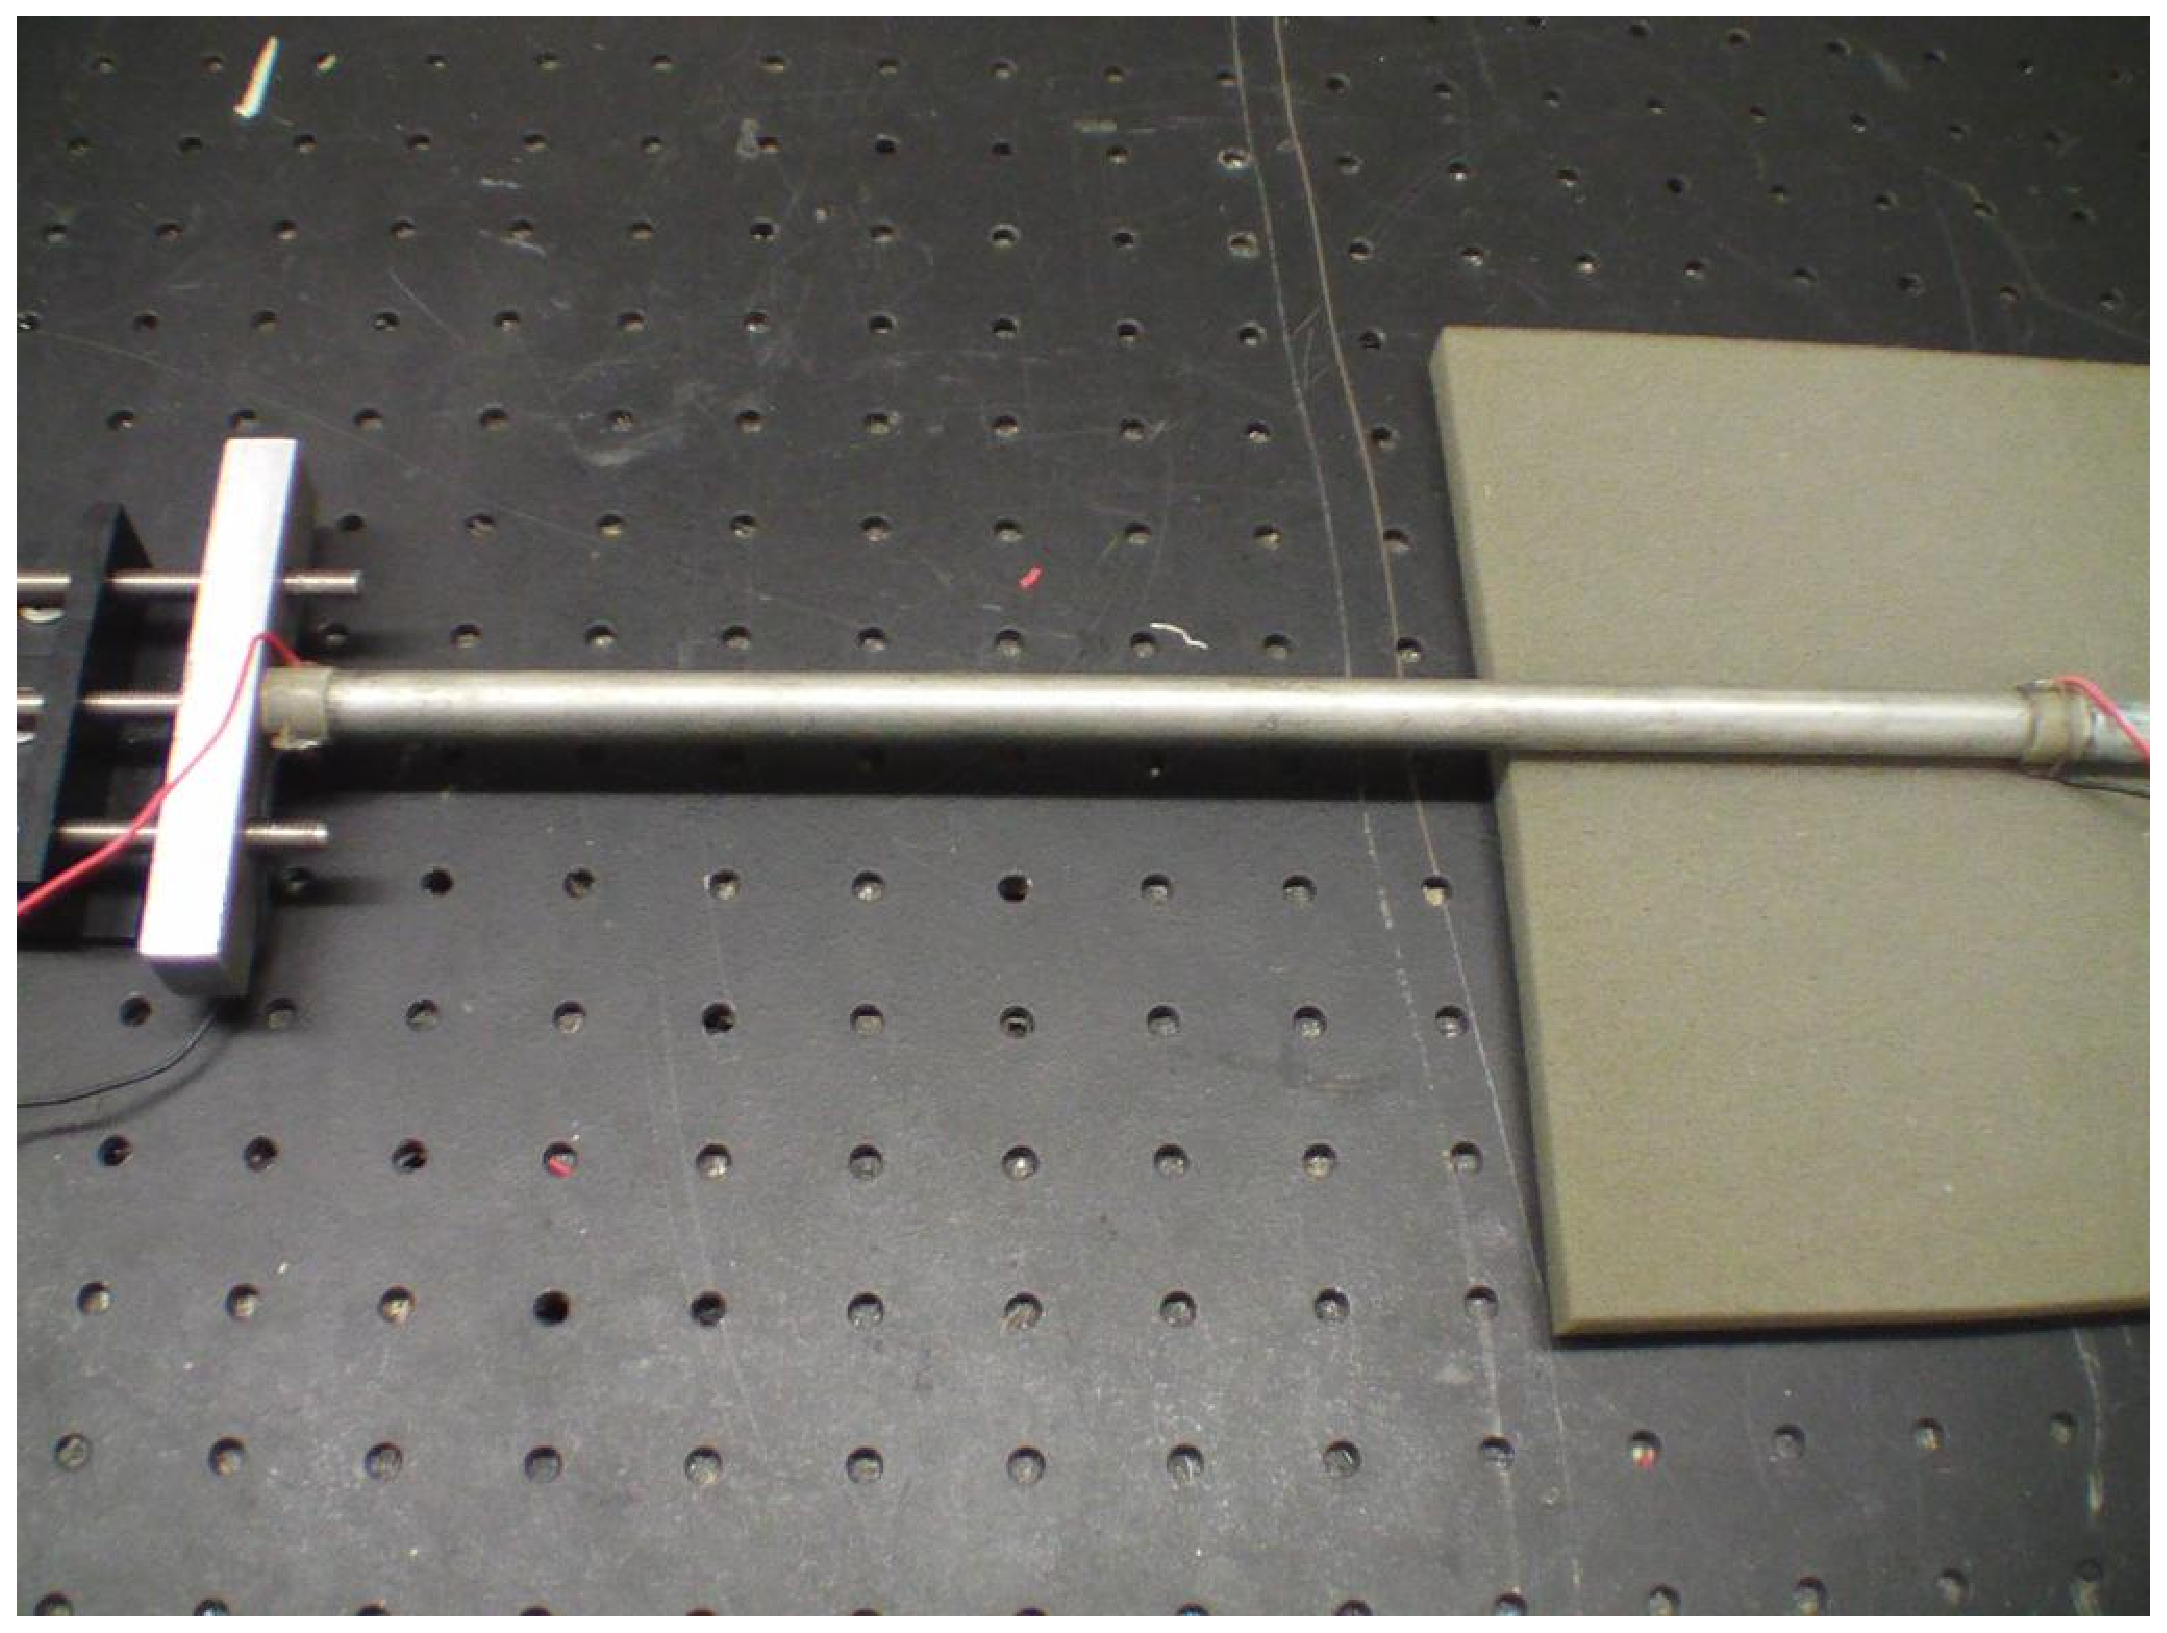
\includegraphics[width=0.6\textwidth]{eps_pics/steelSetupClose}}
\end{subfigmatrix}

   \caption
%>>>> use \label inside caption to get Fig. number with \ref{}
   { \label{fig:steelTR}
(a) One set of steel rods that were used for testing;
(b) Closer view of the left side steel rod (shorter rod) section. The PZT on the right in (b) was the defect PZT and the PZT on the left in (b) was PZT B (not shown is PZT A).
 }
   \end{figure}
   
\begin{figure}
\begin{subfigmatrix}{2}
\subfigure[Full view of steel rod time reversal tests]
{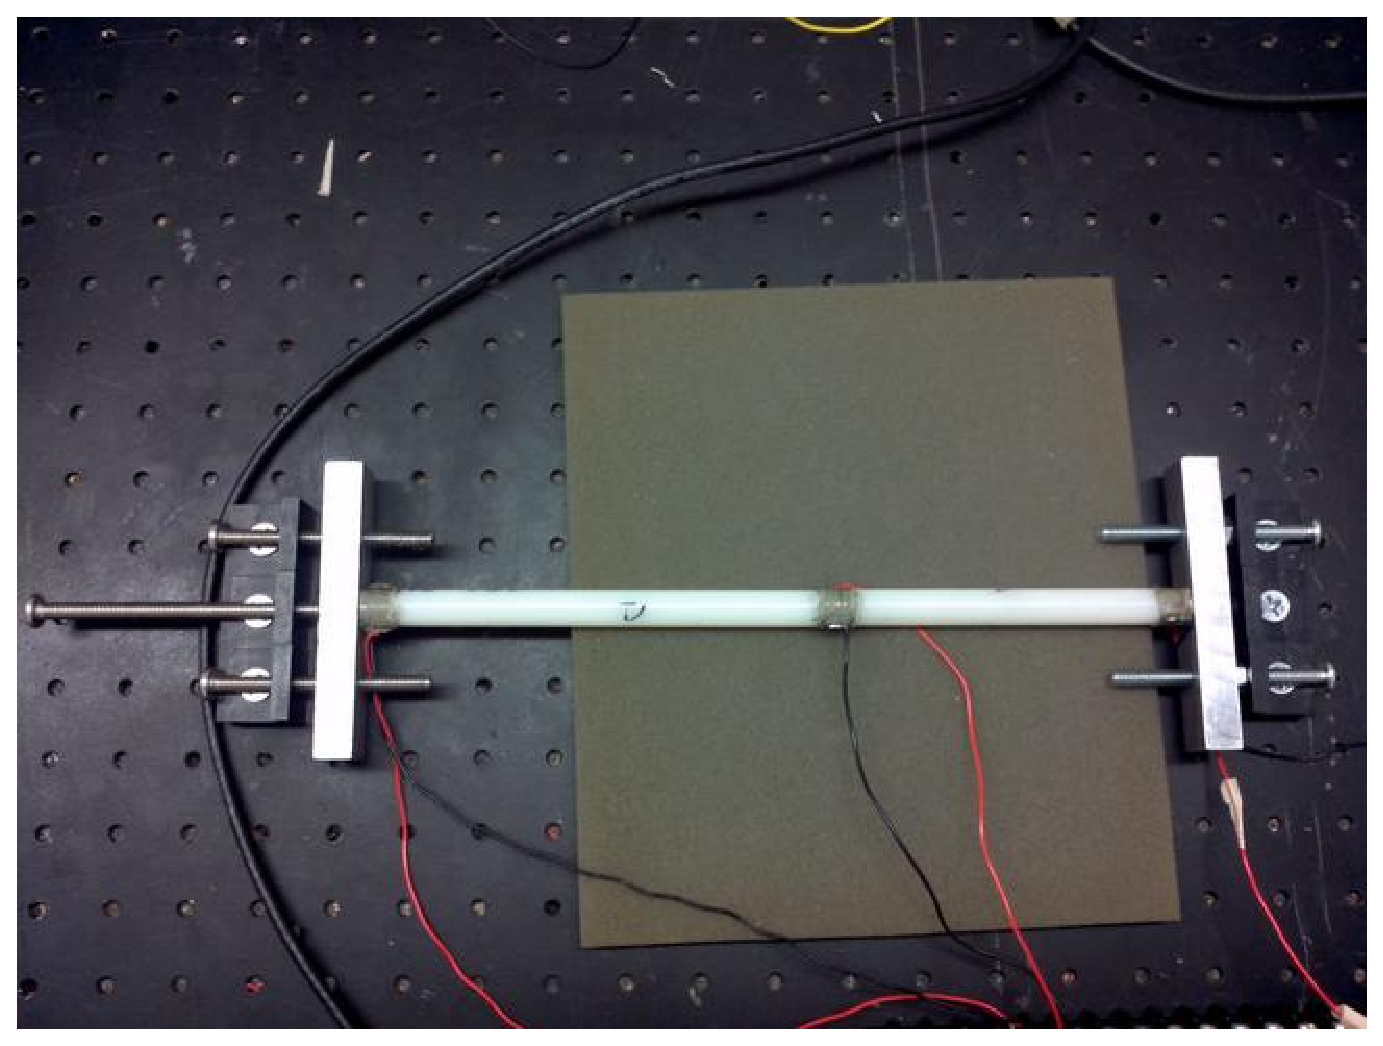
\includegraphics[width=0.6\textwidth]{eps_pics/nylonSetupFull}}
\subfigure[Close up of steel rod time reversal tests]
{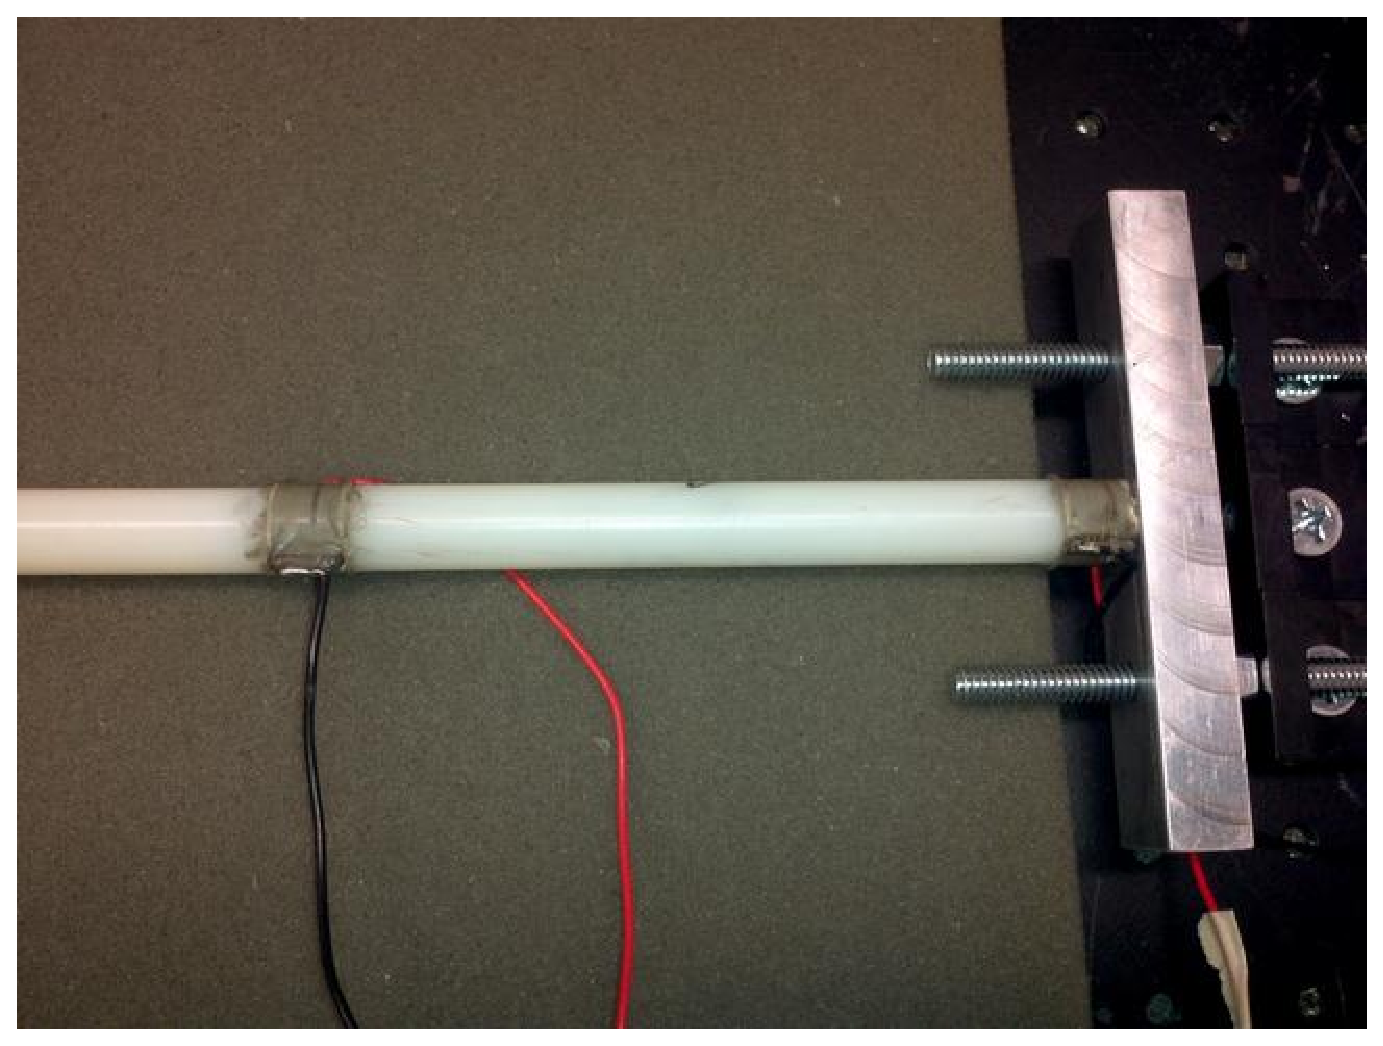
\includegraphics[width=0.6\textwidth]{eps_pics/nylonSetupClose}}
\end{subfigmatrix}

  \caption
%>>>> use \label inside caption to get Fig. number with \ref{}
  { \label{fig:nylonTR}
(a) One set of nylon rods that were used for testing;
(b) Closer view of the right side steel rod (shorter rod) section. The PZT on the left in (b) was the defect PZT and the PZT on the right in (b) was PZT A (not shown is PZT B).
}
\end{figure}

\subsection{Interrogatory Phase}

The first part of the time reversal algorithm is the interrogatory phase. As with the crack detection tests, the host program generated an initial multi-tone wave that was to be played out by PZT A (although the algorithm was indifferent to which PZT plays the initial signal). Before playing out the wave the FPGA zeroed its output values and waited the specified period ($200ms$ here). PZT A sent the wave and simultaneously began recording data. Both the defect PZT and PZT B began also began recording data as the wave was being played by PZT A. The signal propagated through the rod and towards PZT B. On its way to PZT B the wave struck the defect PZT. Upon impacting the defect PZT, the wave was split into multiple components part of which were reflected back towards PZT A and part which continued transmission towards PZT B. The reflected component struck PZT A where it was recorded. The transmitted component reached PZT B where it was also recorded. The components again split upon impacting the boundaries which caused more reflection and transmission components and were also recorded by PZT A and PZT B (Figure \ref{fig:initialPhaseRead}). The recording continued until the desired number of samples for the iteration was reached (2000 samples was chosen here based upon experimental observations). The peak to peak amplitude at the defect PZT was recorded so that it could be compared with the response seen in future iterations.


\begin{figure}
\begin{subfigmatrix}{2}
\subfigure[Response recorded at PZT A in the interrogatory phase]
{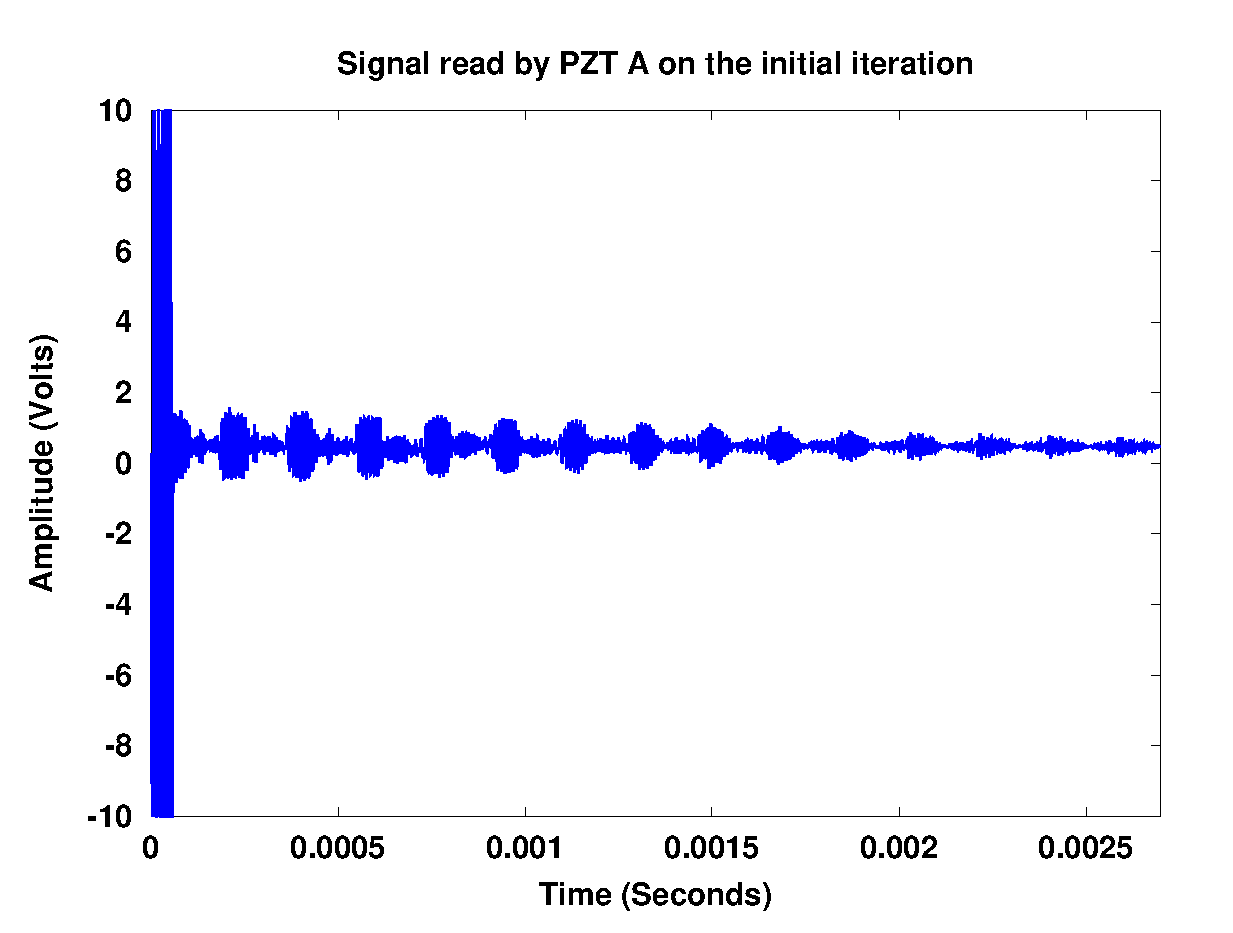
\includegraphics[width=0.6\textwidth]{eps_pics/ch0Read}}
\subfigure[Response recorded at PZT B in the interrogatory phase]
{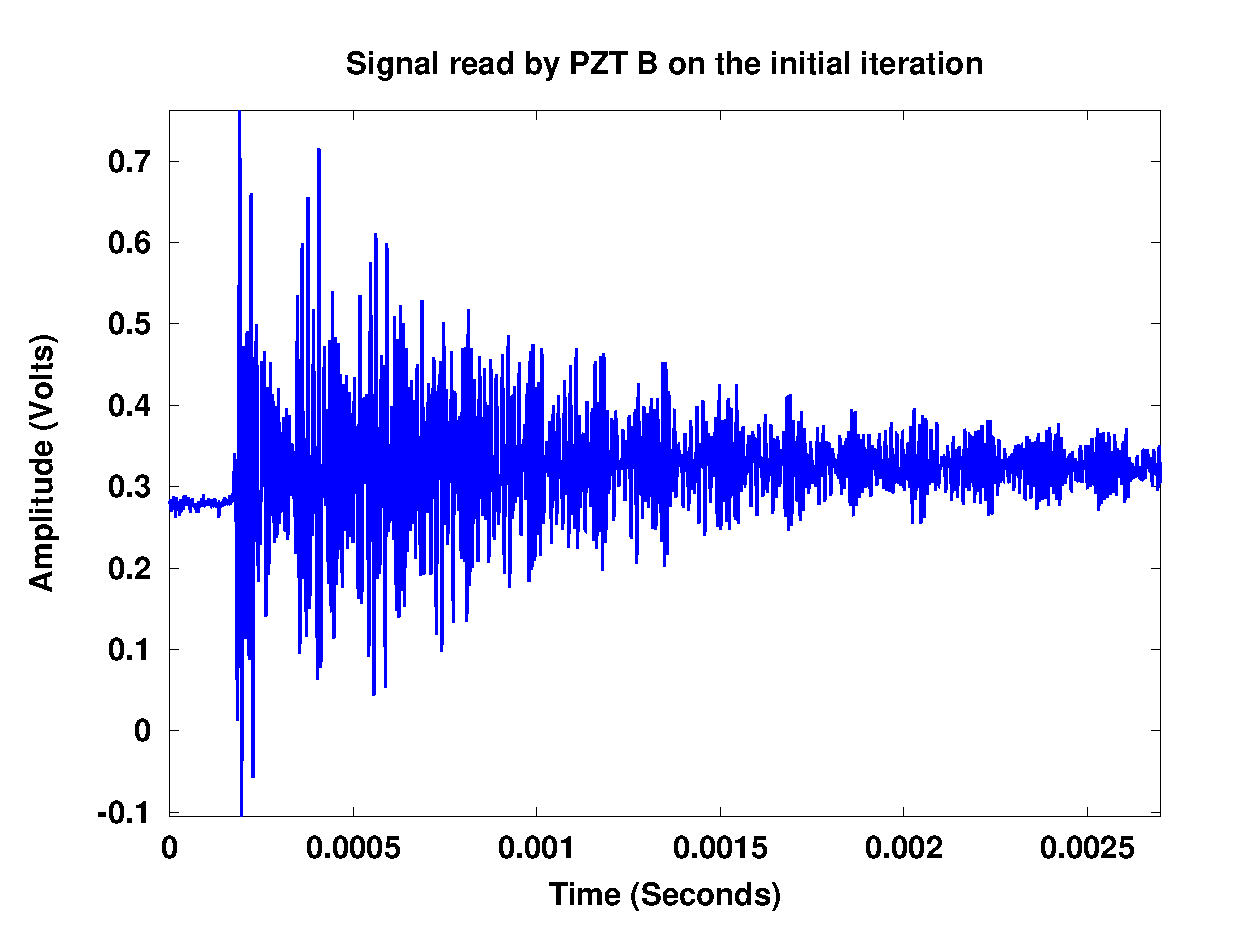
\includegraphics[width=0.6\textwidth]{eps_pics/ch1Read}}
\end{subfigmatrix}

  \caption
%>>>> use \label inside caption to get Fig. number with \ref{}
  { \label{fig:initialPhaseRead}
(a) The response recorded at PZT A (sending PZT) during the interrogatory phase. These tests were carried out using steel rods which were $437 \times 10^{-3} m$ and $428 \times 10^{-3} m$ in length. It is seen that the initial wave played out by PZT A is included in the signal recorded by PZT A and is of substantially higher amplitude than the rest of the data recorded. This was one big difficulty with performing in one dimension. To make the algorithm work, it was necessary to zero out the section of the signal which contained the original wave and also to bypass ringing left over from the PZT playing the wave;
(b) The response recorded at PZT B (opposite end) during the initial iteration.
}
\end{figure}

\subsection{Selection Phase}

The next step in the time reversal algorithm is the selection phase. During the selection phase it is determined which portion of each recorded signal should be reversed and played back. Typically for multi-dimensional time reversal the setup allows for the entire recorded signals to be used during playback. With one dimensional time reversal, however, it is important that only a portion of this signal be sent back. This becomes more apparent in the iterative time reversal case which is discussed later. For the signal read by PZT A, the window extracted contained the occurrence of the first reflection component of the initial wave. With PZT B it was the window containing the occurrence of the first transmitted component of the initial wave. To extract the signal portions to reverse the data recorded by each PZT during the interrogatory phase were transferred from the FPGA to the host computer and then processed. A windowed root mean square (RMS) was performed on the signal read by PZT A. The window size used was 40 data points and was based upon the initial wave size of 40 data points. A single value was computed for each RMS window which corresponded to the energy concentration found in the signal during that sampling window. The collection of RMS values were stored in an array. When plotted, this array is seen to essentially draw a line around the wave groupings found within the signal for PZT A. The local maximums in the RMS plot correspond to the occurrence of high energy stress-waves at PZT A. Since PZT A played out the initial signal it was required to zero out the first part of its recorded signal so that the PZT vibrations from the wave being played did not overshadow the rest of the data. The zero period was specified at program start up and was chosen to be 100 points which was a little more than twice the length of the original wave played. After zeroing out the beginning of the signal the first local maximum in the signal was indicative of the first reflection component arriving at PZT A (Figure \ref{fig:windowedRMS}). The window centered on this peak was extracted for reversal. A window was extracted from PZT B's signal using the same algorithm.


\begin{figure}
\begin{subfigmatrix}{2}
\subfigure[PZT A Windowed RMS]
{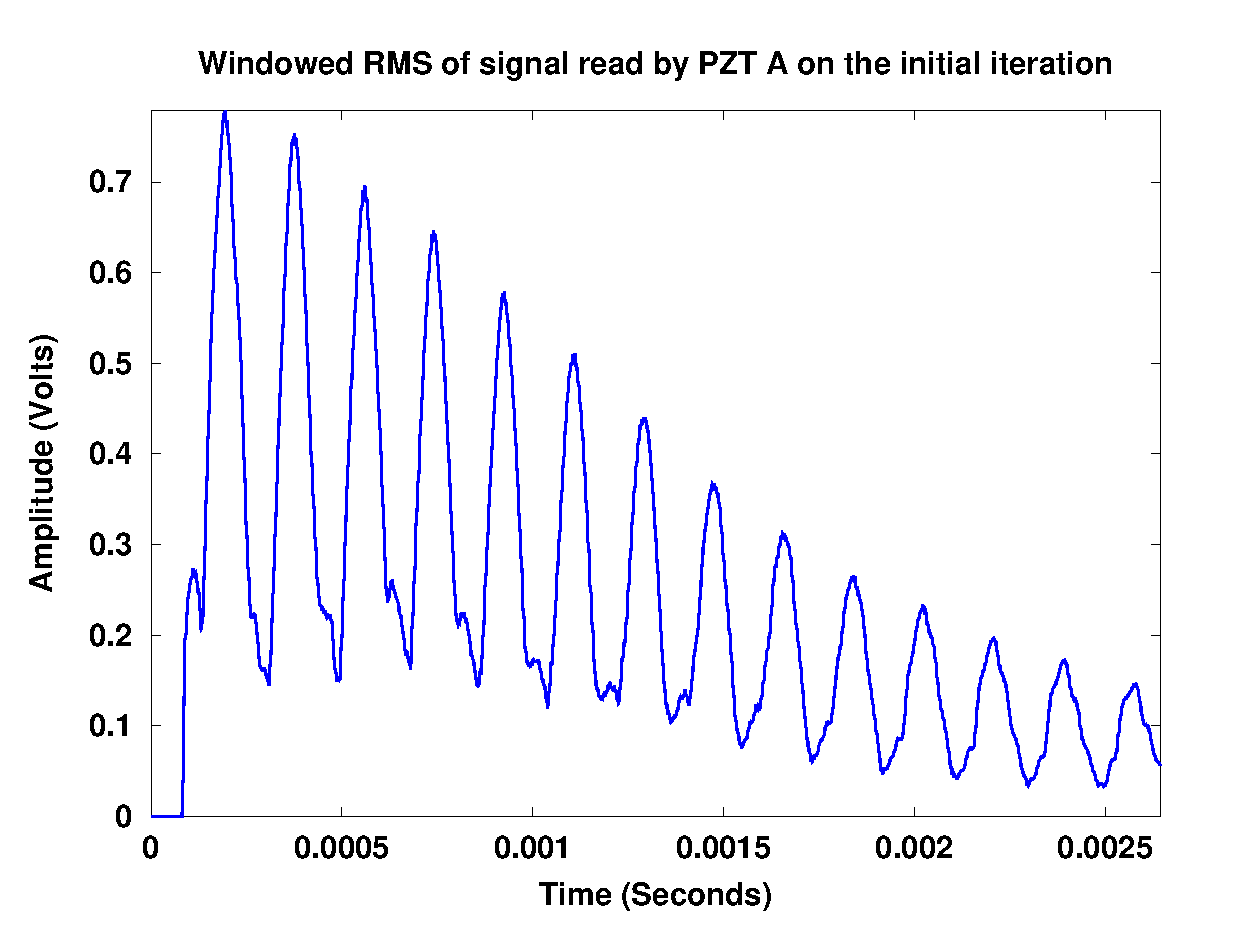
\includegraphics[width=0.6\textwidth]{eps_pics/ch0RMS}}
\subfigure[PZT B Windowed RMS]
{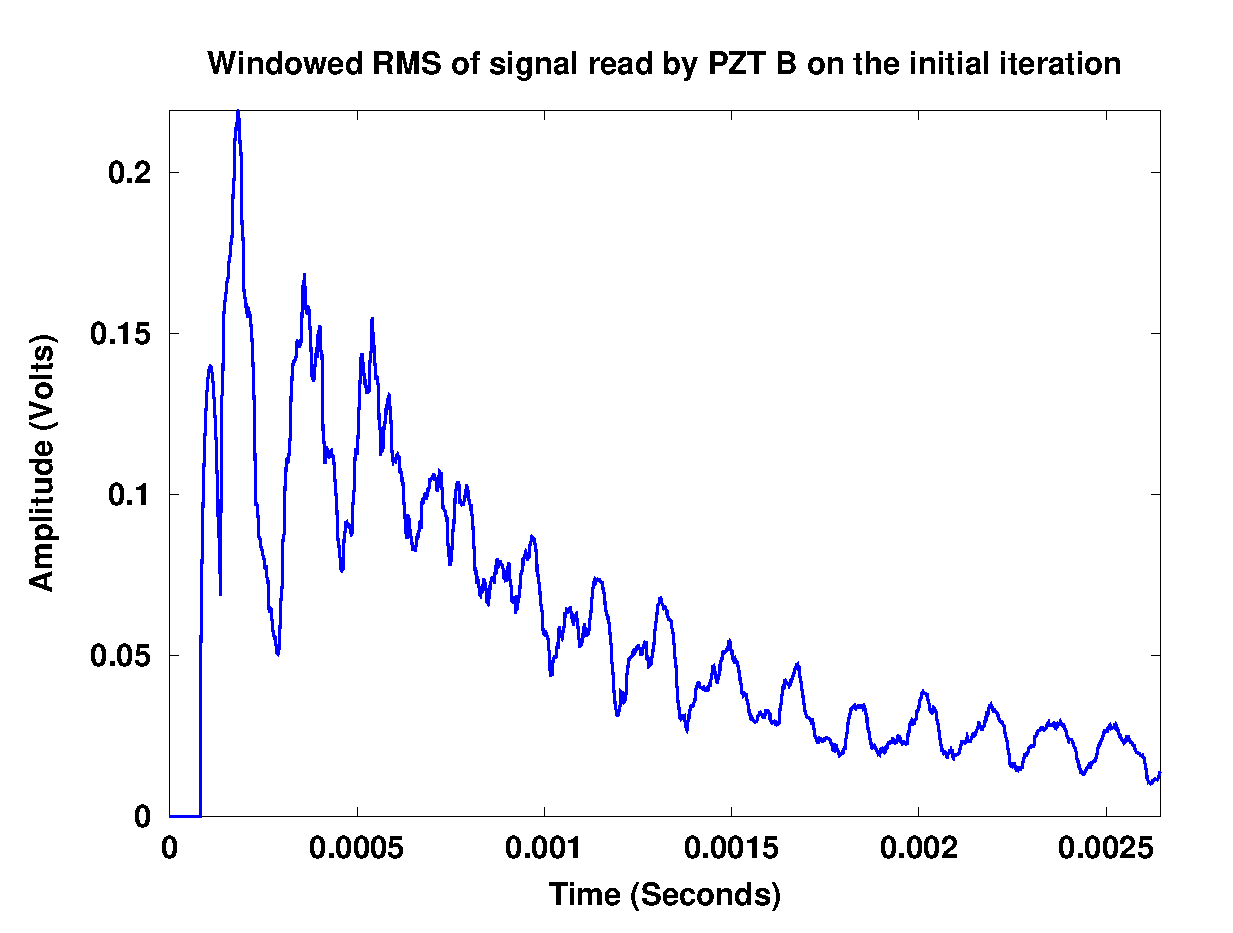
\includegraphics[width=0.6\textwidth]{eps_pics/ch1RMS}}
\end{subfigmatrix}

  \caption
%>>>> use \label inside caption to get Fig. number with \ref{}
  { \label{fig:windowedRMS}
(a) Windowed RMS of PZT A's signal using a window length of 40 data points. Since PZT A played a signal while recording, the first 100 points were zeroed so that the rest of the data could be seen. The largest point for this test was found to be around the 144th data point and marked the start of the window that was extracted and played back by PZT A;
(b) Windowed RMS of PZT B's signal which had the largest peak occur around the 136th data point.
}
\end{figure}

The window extracted from PZT A's signal was 60 data points in length and was based upon the original wave size of 40 points which left room for error in terms of the wave's location in the signal. The extracted length also had to be small enough so that it did not include any responses not produced by the initial reflection component. This extracted window was centered on zero, scaled to be maximum amplitude, and then time reversed so that last data point became the first and vice-versa. The same procedure was follow for the window extracted from PZT B's signal (Figure \ref{fig:chosenSignals}).

\begin{figure}
\begin{subfigmatrix}{2}
\subfigure[PZT A Selected Window]
{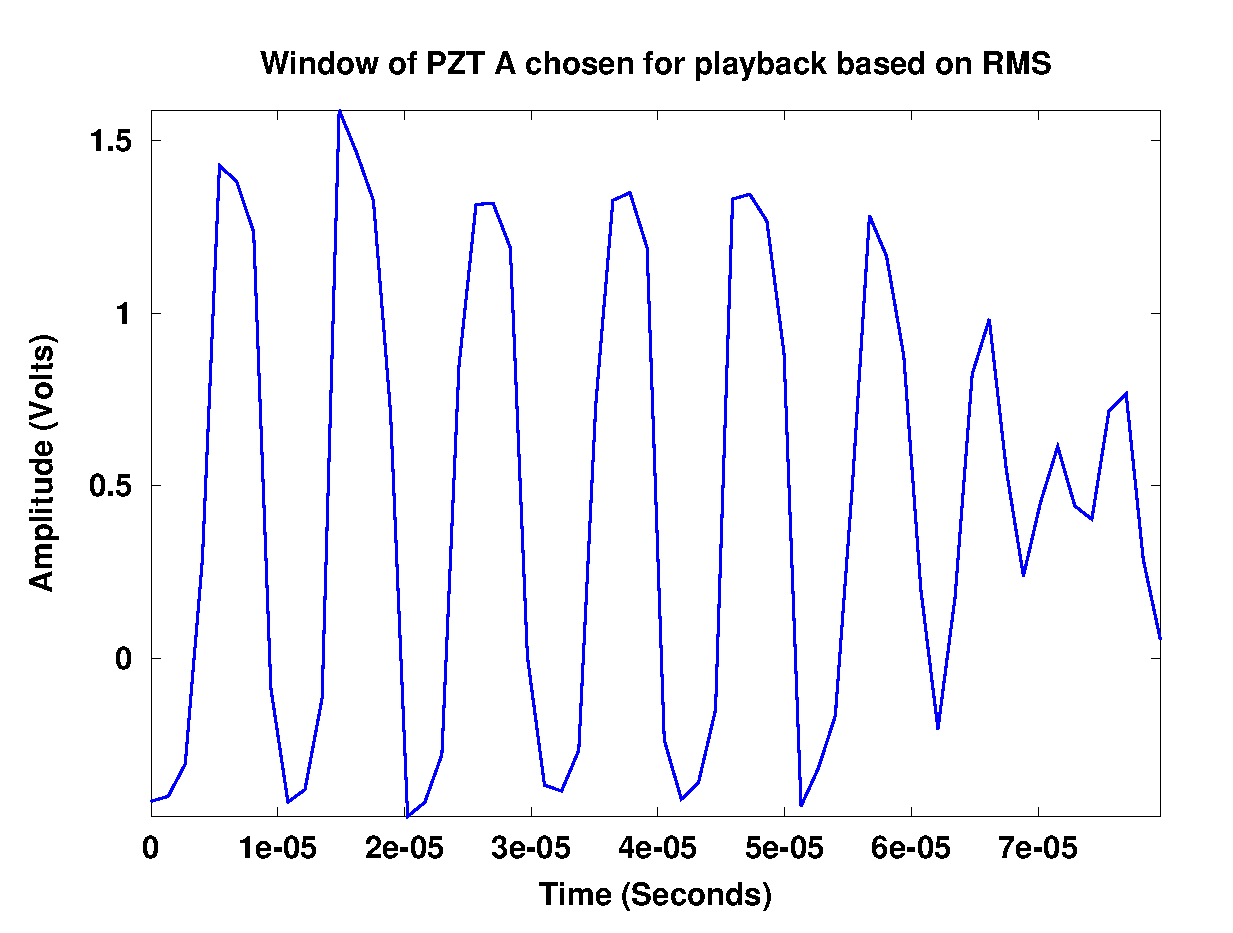
\includegraphics[width=0.6\textwidth]{eps_pics/ch0Chosen}}
\subfigure[PZT B Selected Window]
{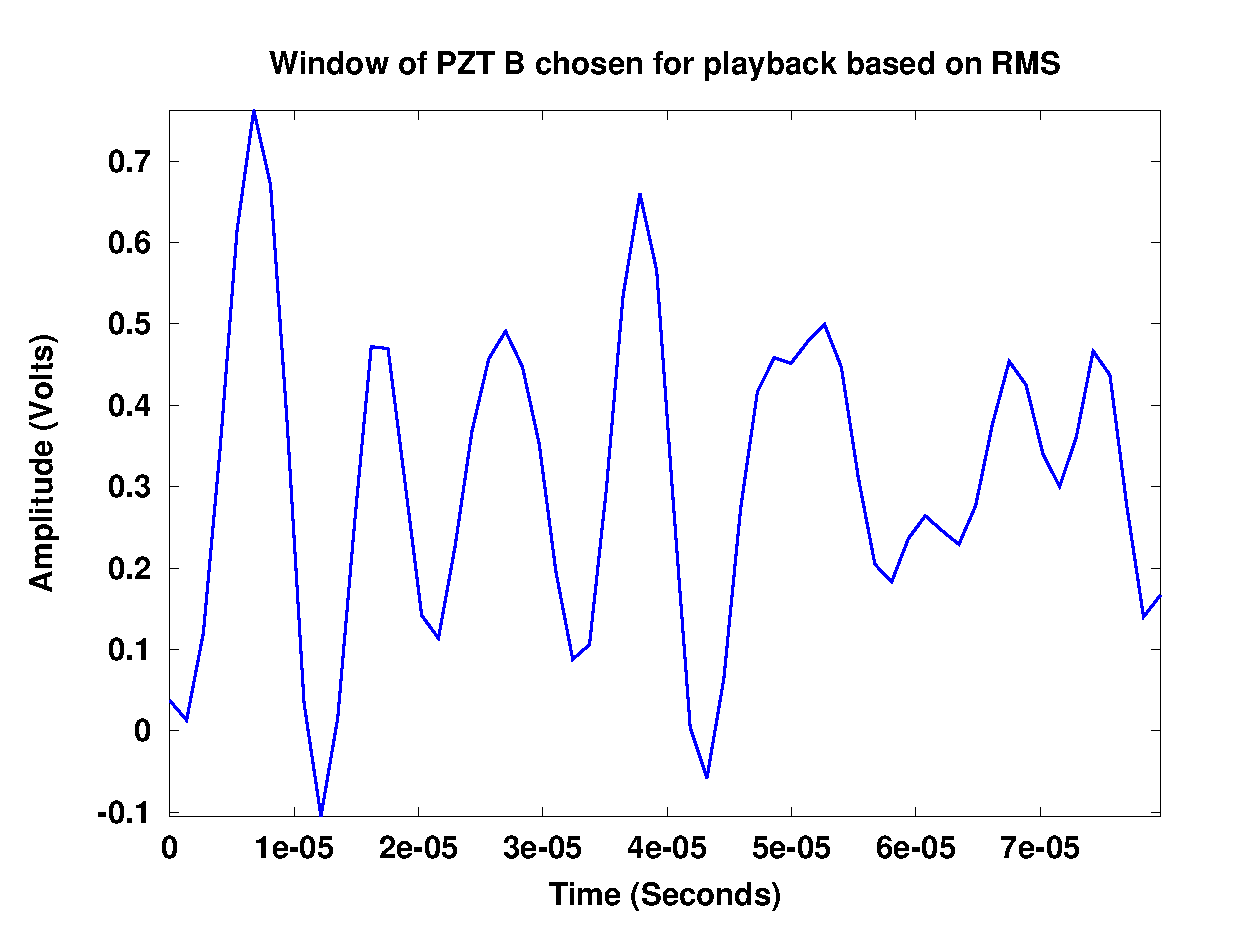
\includegraphics[width=0.6\textwidth]{eps_pics/ch1Chosen}}
\end{subfigmatrix}

  \caption
%>>>> use \label inside caption to get Fig. number with \ref{}
  { \label{fig:chosenSignals}
(a) Window of PZT A's signal that was chosen for playback and is based upon the maximum peak found in the windowed RMS graph for the signal read by PZT A;
(b) Window of PZT B's signal that was chosen for playback and used the same selection algorithm that selected PZT A's playback window.
}
\end{figure}

Once the windows were selected and processed for playback it was necessary to determine which window occurred first in terms of the global time domain. This step is needed because no a priori knowledge of the rods' length is assumed and a zero period must be played out by one of the PZTs during playback. The zero period played by one of the transducers is what allowed for the signals played back by each PZT to arrive at the crack simultaneously. In this sample test it was found that PZT B had the first wave occurrence at the 136th data point whereas PZT A's occurred at the 144th data point.  The zero period was chosen to be the difference in arrival times (here, 144 - 136 = 8) and this period was inserted at the beginning of PZT B's signal. In order to have consistent playback signal lengths an equal zero period was appended to PZT A' playback signal (Figure \ref{fig:scaledSignals}).

\begin{figure}
\begin{subfigmatrix}{2}
\subfigure[PZT A Selected Window]
{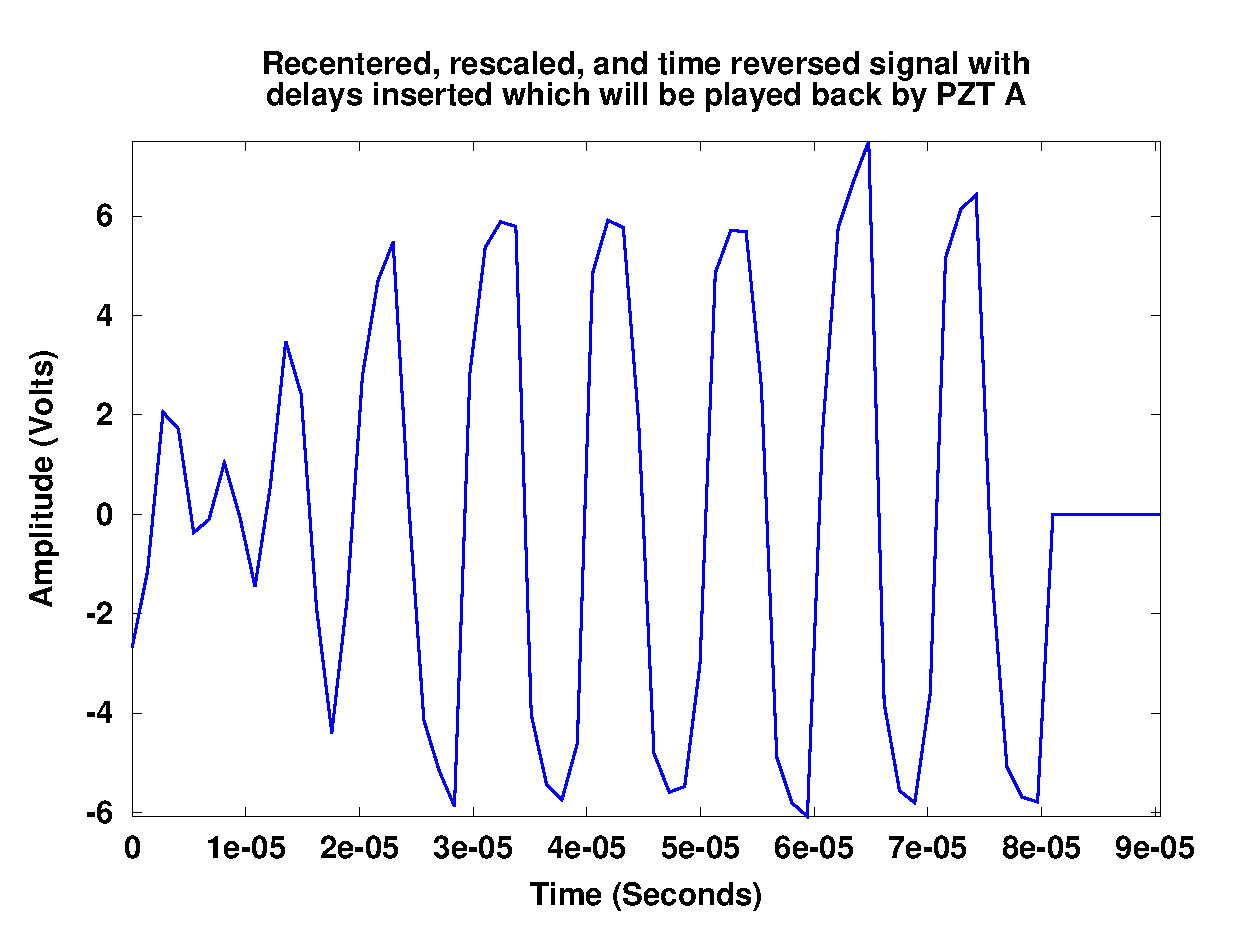
\includegraphics[width=0.6\textwidth]{eps_pics/ch0Scaled}}
\subfigure[PZT B Selected Window]
{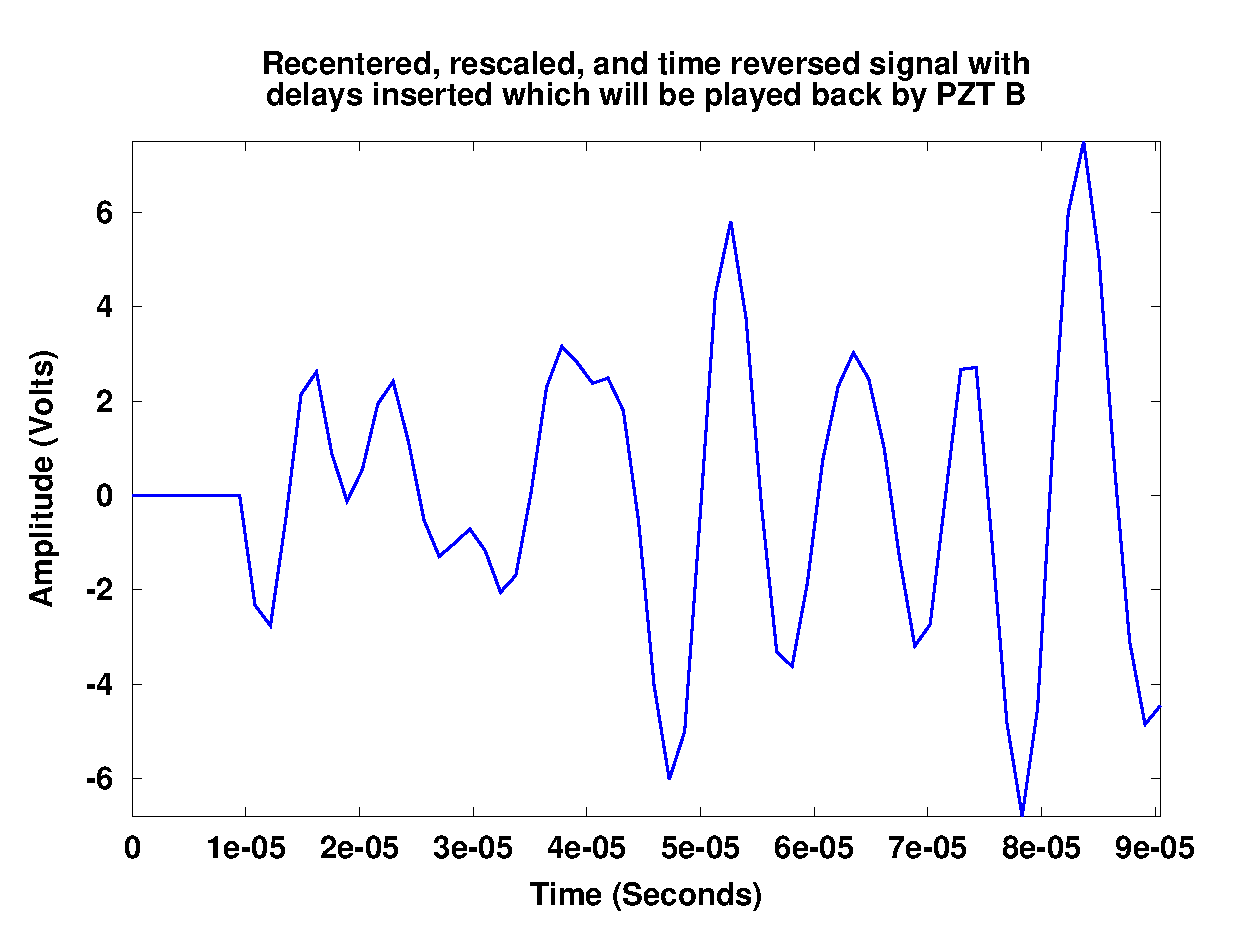
\includegraphics[width=0.6\textwidth]{eps_pics/ch1Scaled}}
\end{subfigmatrix}

  \caption
%>>>> use \label inside caption to get Fig. number with \ref{}
  { \label{fig:scaledSignals}
(a) Window played back by PZT A during the time reversal phase which has been centered on zero, scaled to max amplitude, and time reversed;
(b) Window played back by PZT B during the time reversal phase which has also been centered on zero, scaled, and time reversed. A zero period was inserted at the beginning of PZT B's playback window in order for the signals played by each PZT to arrive at the defect at the same instant. This zero period was needed because the crack was closer to PZT B than PZT A and was a priori unknown but was inferred from the data recorded.
}
\end{figure}

\subsection{Time Reversal Focusing Phase}
After selecting and processing the windows for playback it was time for the time reversal focusing phase. The processed windows were transferred from the host program to the FPGA program. Before playing back the signals the FPGA waited for a period of $200ms$ to allow for the ringing in the rod to decay. Following the idle period both PZT A and PZT B played their respective windows. These waves traveled through the through the rod and simultaneously reached the defect PZT. Upon reaching the defect the wave energies combined and a focusing occurred at that location. The peak to peak amplitude at the defect PZT was recorded and compared to the initial iteration.

\subsection{Iterative Time Reversal}
The time reversal process was performed in an iterative fashion. The iterative algorithm was identical to the previously described time reversal algorithm up through the Time Reversal Focusing Phase. The extension was that during the time reversal phase, PZT A and PZT B began recording data as soon as they started playing their signals. Windows were again extracted from each signal for playback. This time, however, it was not necessary to perform the windowed RMS on each signal in order to determine which window to extract. The extraction point information from the first selection phase was used to extract a playback window from each signal. As mentioned previously, the iterative time reversal algorithm is where it is important that we play back only a selected portion of the signal and not the entire signal since the PZTs must record information on the same iteration in which they send signals. If the playback signals were to be arbitrarily long then any new information would be overshadowed by the playing out of the signal. These extracted windows were again centered on zero, scaled to max amplitude, time reversed, and the necessary zero periods were inserted. The same time reversal focusing phase was performed as described before with the FPGA idling for $200ms$ before playing out the signals in order to let the rod ringing decay. The entire algorithm was then repeated with new information being recorded by each PZT, being processed, and then being played back. With each playback a better focusing is achieved at the defect site. This process continued for 150 iterations which was found to be the point at which little change was seen in the response at the defect PZT. The flow chart for the iterative time reversal algorithm is shown in Figure \ref{fig:newFlow}.

\begin{figure}[ht!]
\centering
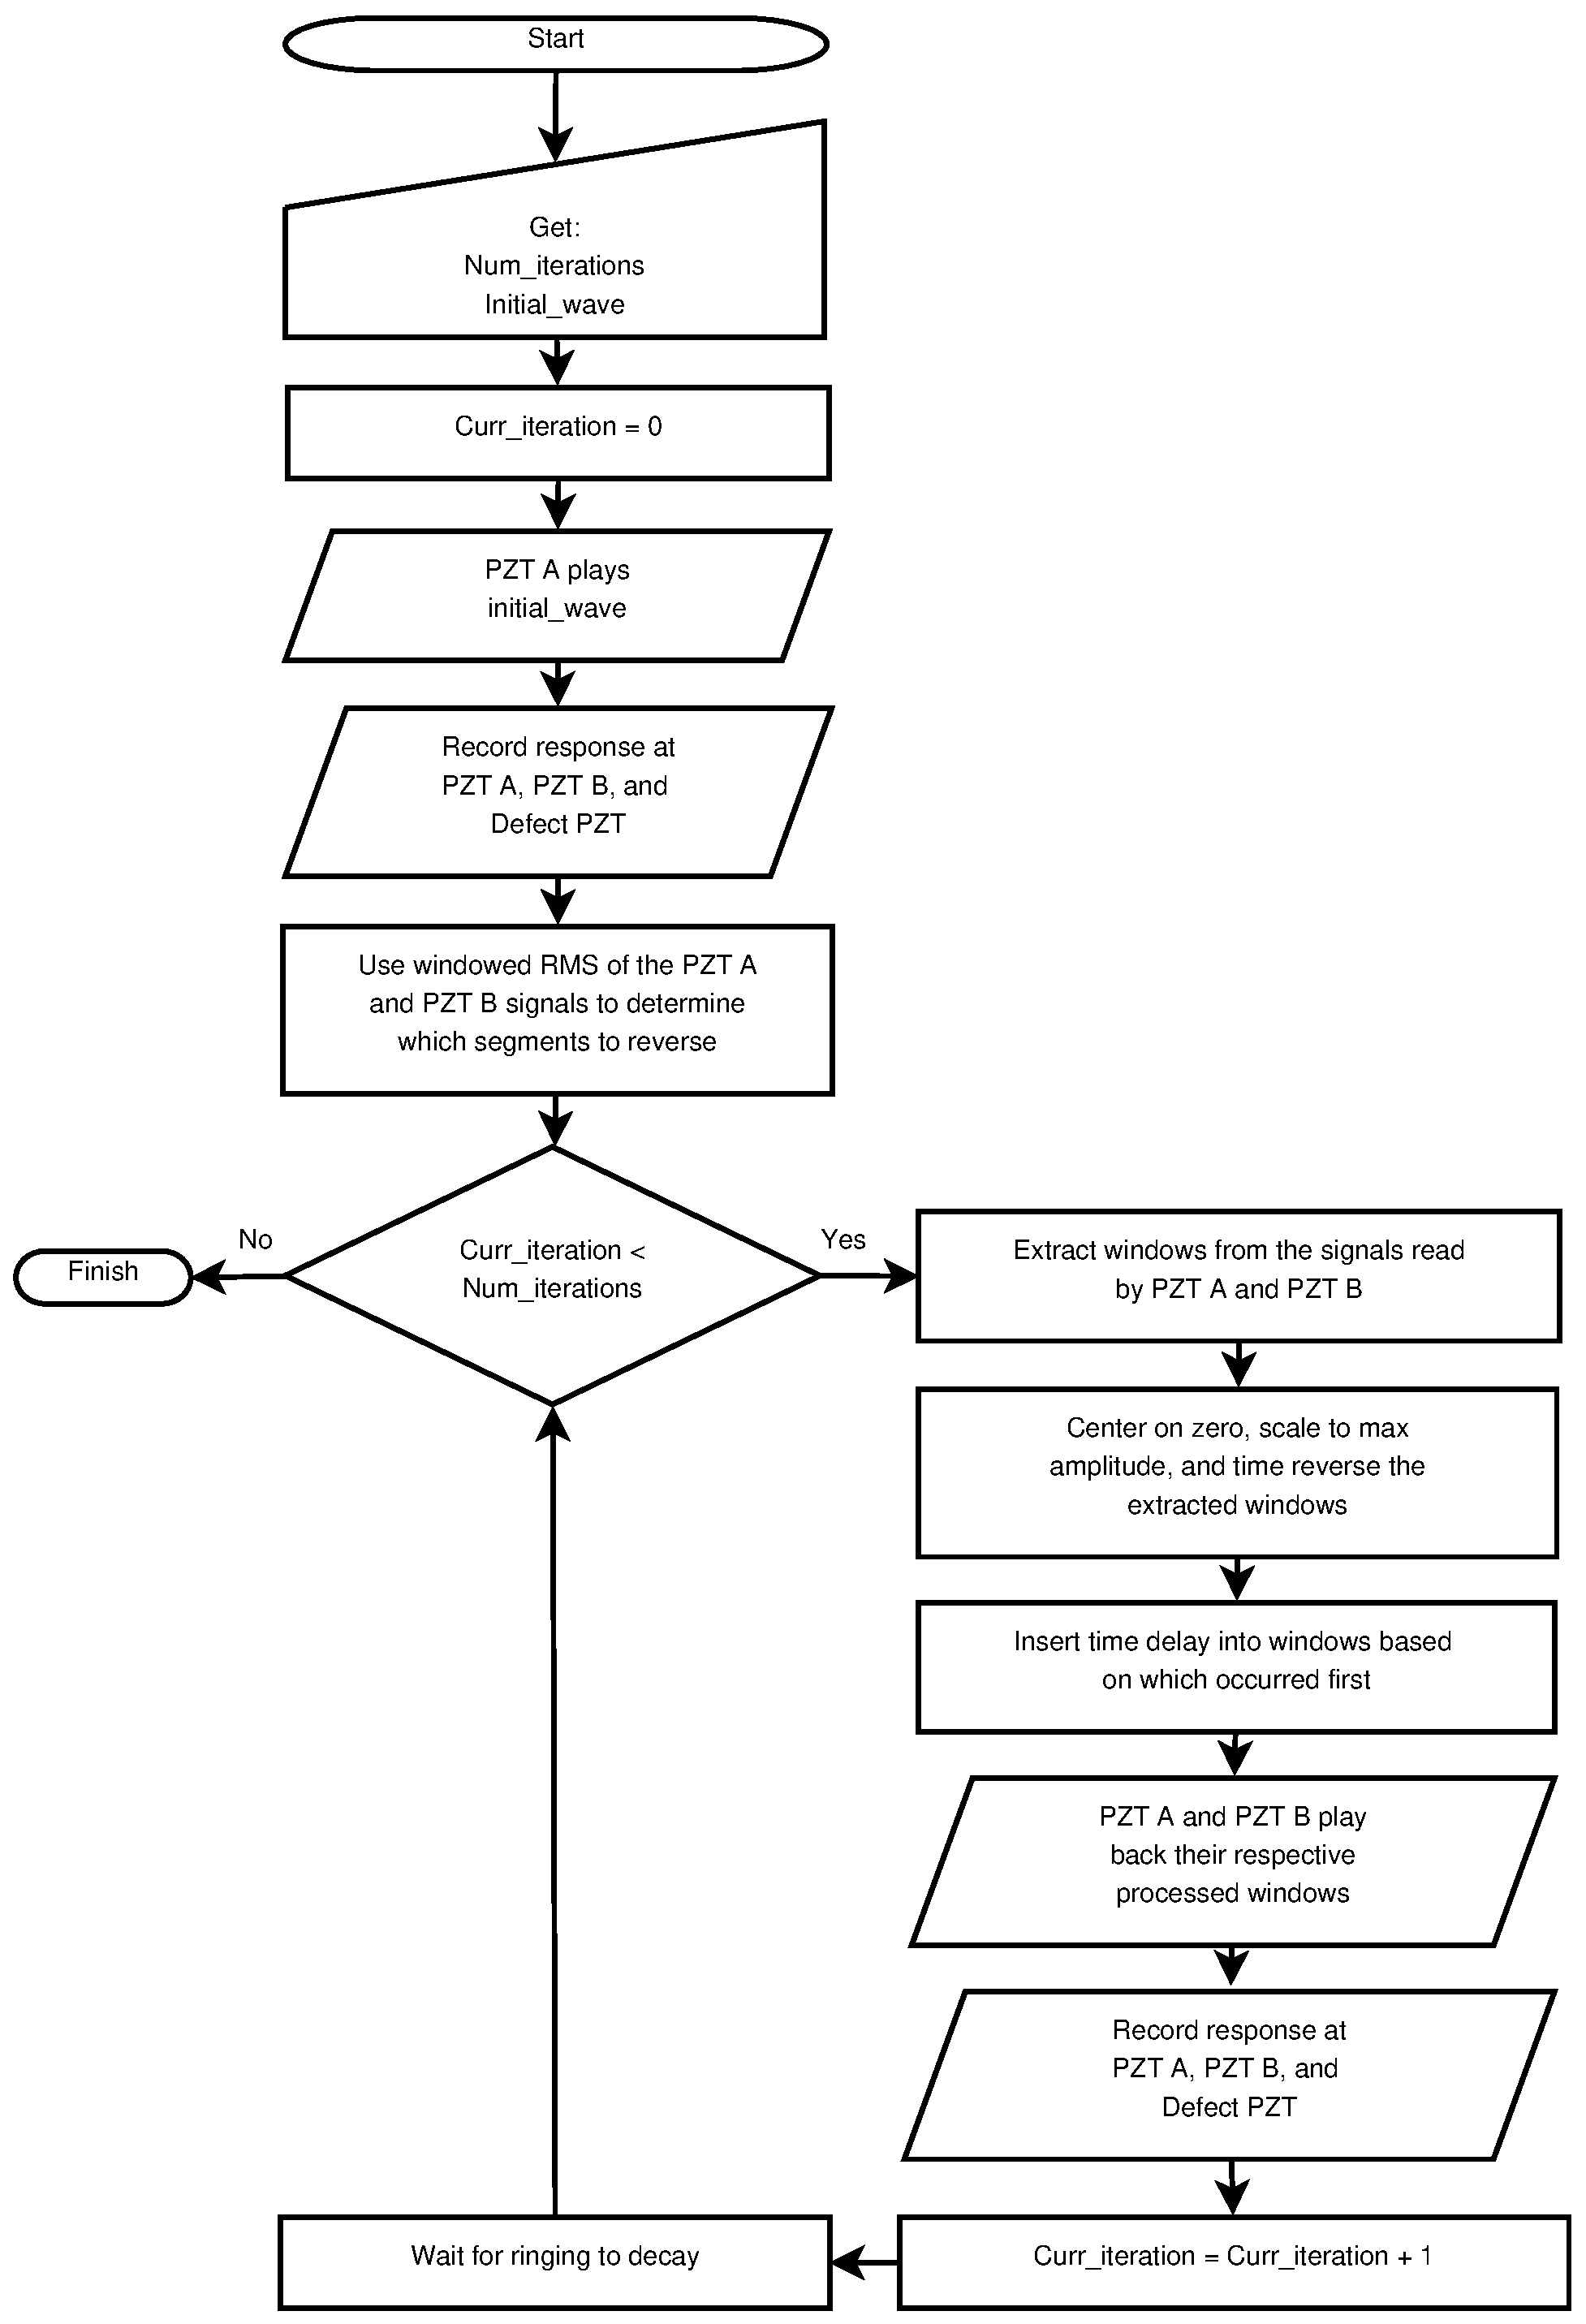
\includegraphics[width=1.0\textwidth]{eps_pics/newFlow}
\caption{Logic flow diagram for the time iterative time reversal algorithm.
 	 \label{fig:newFlow}} 
\end{figure}


\chapter{Results}\label{ch:Results}
%Results

In this chapter the results from each of the experiments are detailed. Signals that were read with and without using the diode circuit are shown. The experimental results for the single iteration time reversal algorithm are compared with the theoretical results from the model described earlier. The crack detection and iterative focusing results are also examined.

\section{Diode Damping Circuit}
It was found experimentally that the amplifier circuits used produced enough noise to be a nuisance during testing. To address this problem a simple diode circuit was designed to snuff out low voltage noise at the expense of reduced output amplitude. The voltage damping is due to the voltage drop that occurs across the diode which effectively blocks voltages lower than about $0.8V $ for the diodes chosen. A nylon rod section of $148 mm$ was used for the test. PZT A sent a signal and PZT B recorded. The results with and without the diode circuit are compared in Figure \ref{fig:diodeCircuitResults}. It was seen the using the diode circuit produced a much cleaner signal recording.

\begin{figure}[ht!]
\begin{subfigmatrix}{2}
\subfigure[Signal recorded by PZT B without the diode circuit]
{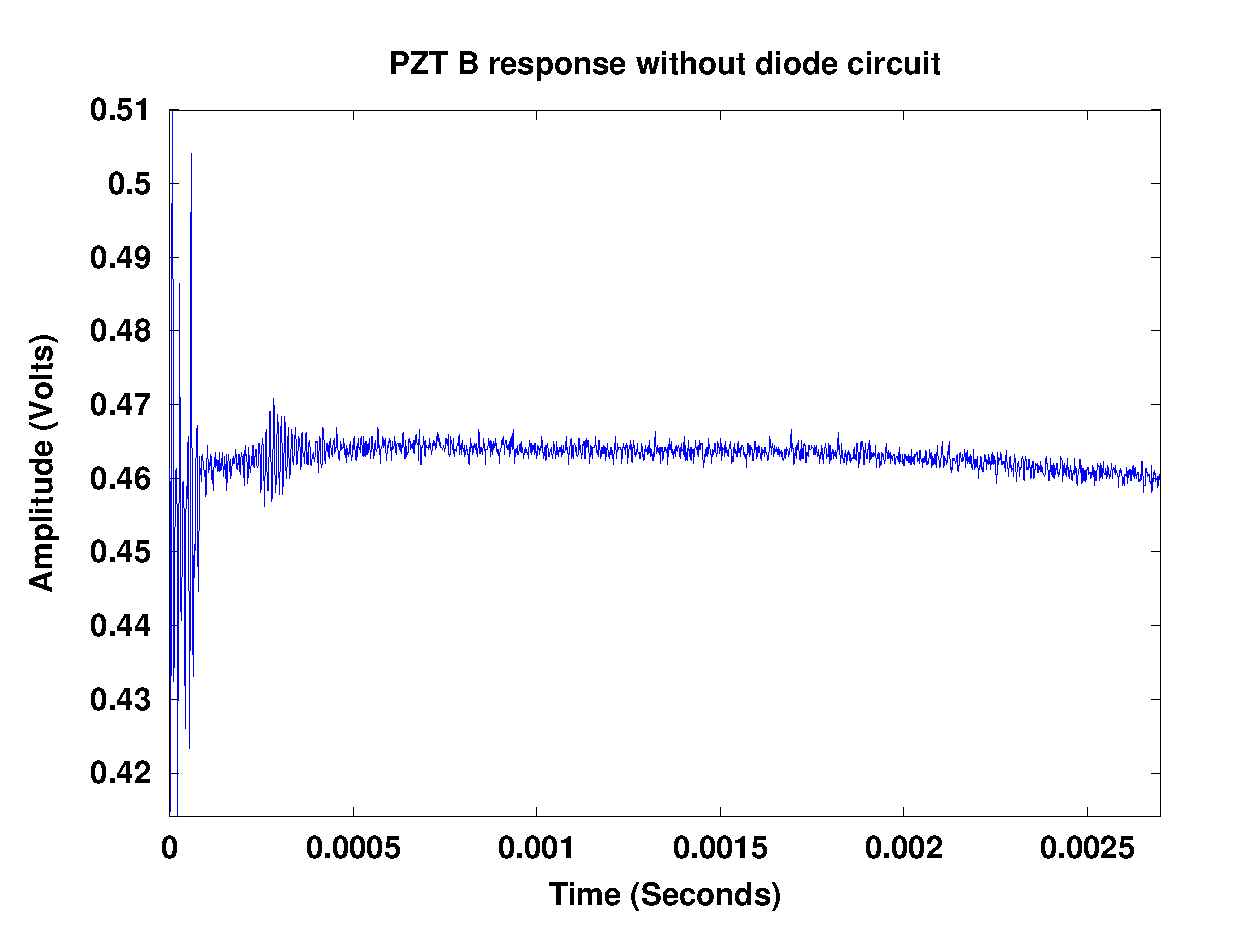
\includegraphics[width=0.6\textwidth]{eps_pics/noCircuit}}
\subfigure[Signal recorded by PZT B with the diode circuit]
{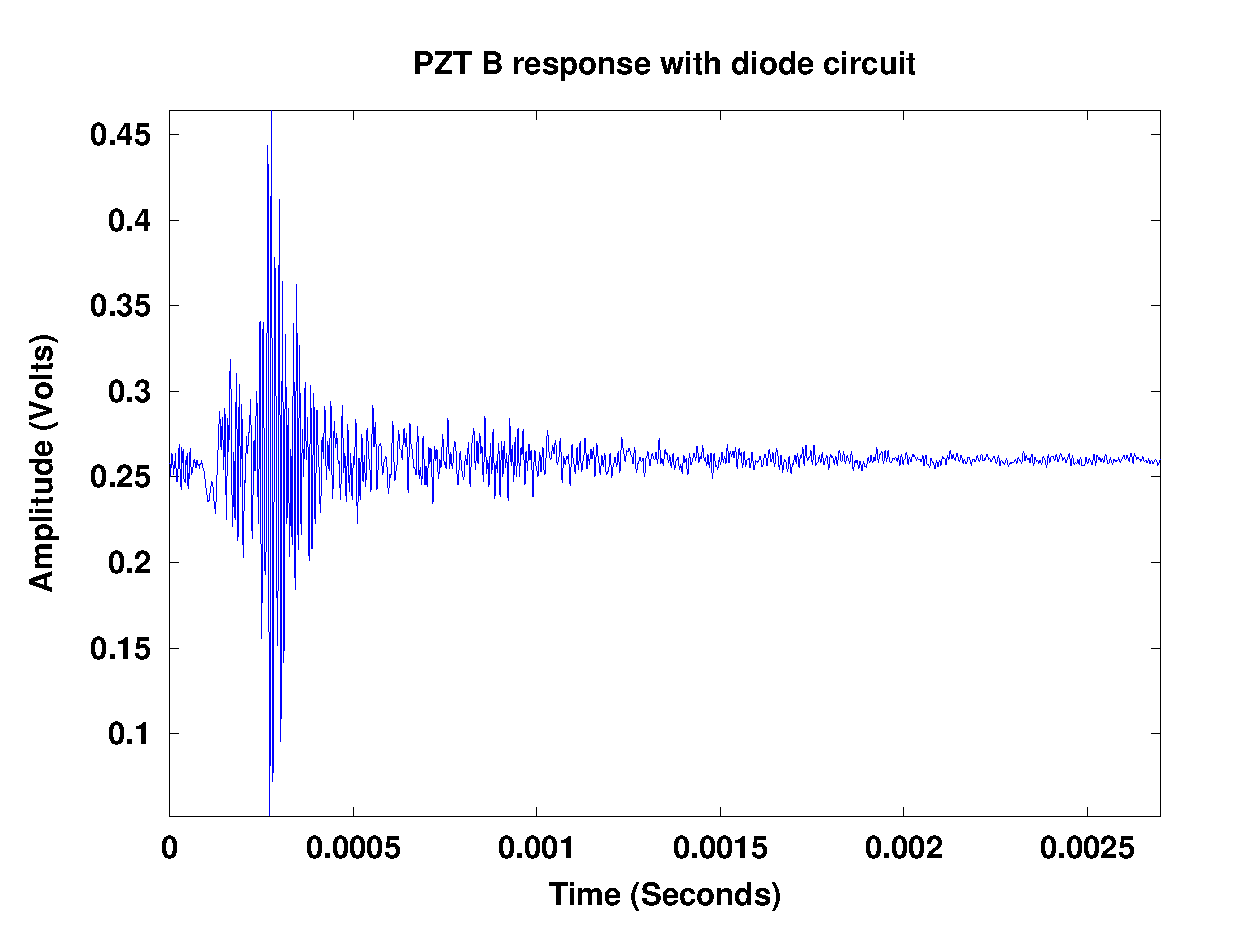
\includegraphics[width=0.6\textwidth]{eps_pics/withCircuit}}
\end{subfigmatrix}

  \caption
%>>>> use \label inside caption to get Fig. number with \ref{}
  { \label{fig:diodeCircuitResults}
(a) Signal recorded at PZT B when the diode circuit was not being used;
(b) Signal recorded at PZT B when the diode circuit was in place. It was seen that there was a large difference between the signals in (a) and (b). The wave seen in (b) was still present in (a) but was largely overshadowed by the amplifier noise.
}
\end{figure}

\section{Crack Detection Results}
The crack detection experiments were to prove that the program could detect when damage occurred within a rod. Signals were sent from PZT A and propagated through the rod where they were recorded on the other end by PZT B. The first set of tests were performed using the steel rods. The graphs of the undamaged and damaged rod tests are shown in Figure \ref{fig:steelCrackResults}. It is seen that the wave recorded by PZT B during the damaged rod tests is substantially smaller in amplitude than the wave that is recorded in the undamaged rod tests. The tests were run five times for both the undamaged and damaged samples. The signal recorded for the first test for the undamaged rod was taken to be the initial rod state. The remaining nine test signals were then compared to this first signal to determine the change in signal which was taken as the sum of squared differences between the signals being compared. The results from each comparison are shown in Figure \ref{fig:steelDifferences} where the damaged rod is introduced on the 6th iteration. It is seen that there is a very large jump in the computed signal difference when the damaged rod signal data is introduced. 

\begin{figure}[ht!]
\begin{subfigmatrix}{2}
\subfigure[PZT B Signal Undamaged Steel Rod]
{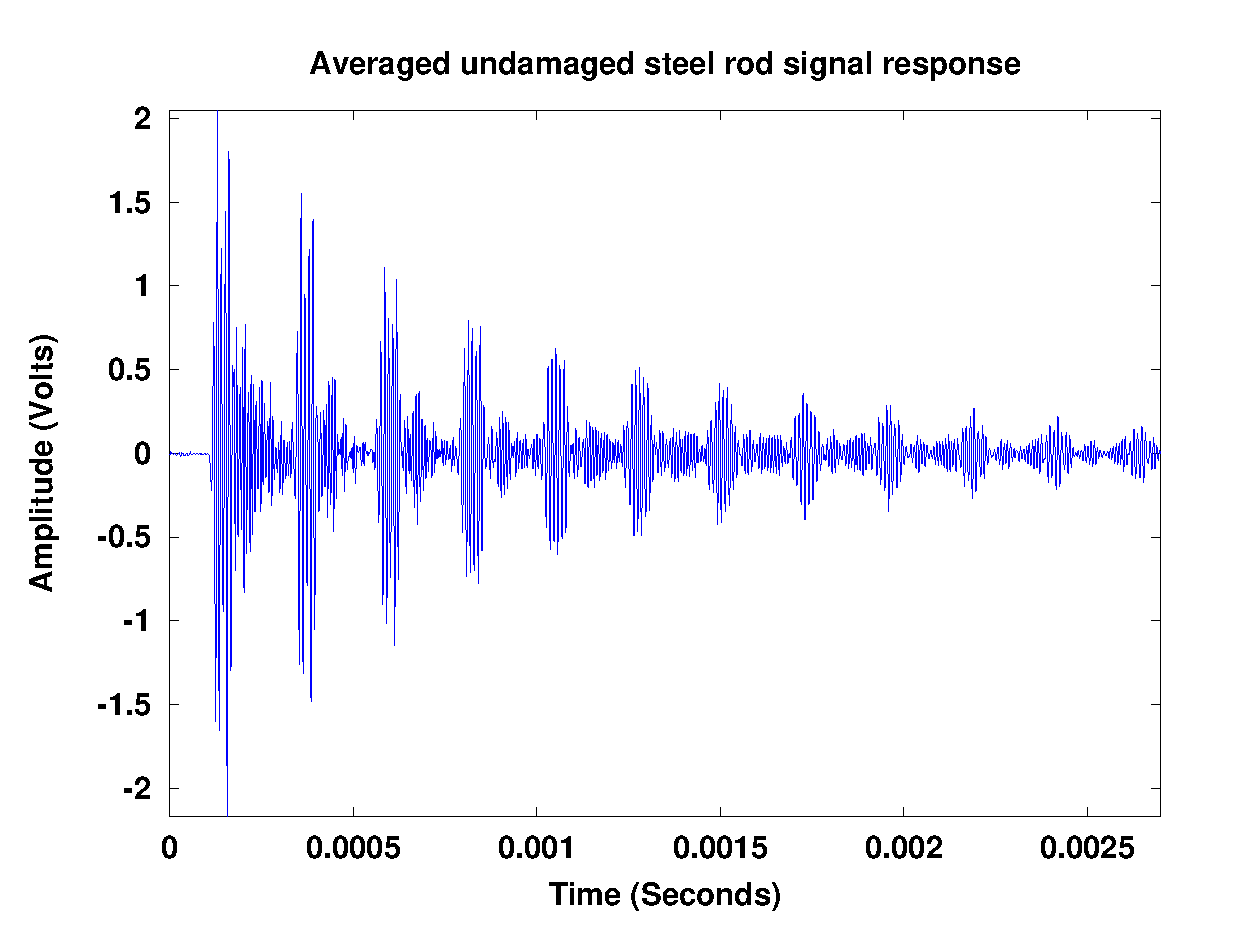
\includegraphics[width=0.6\textwidth]{eps_pics/steelUncracked}}
\subfigure[PZT B Signal Damaged Steel Rod]
{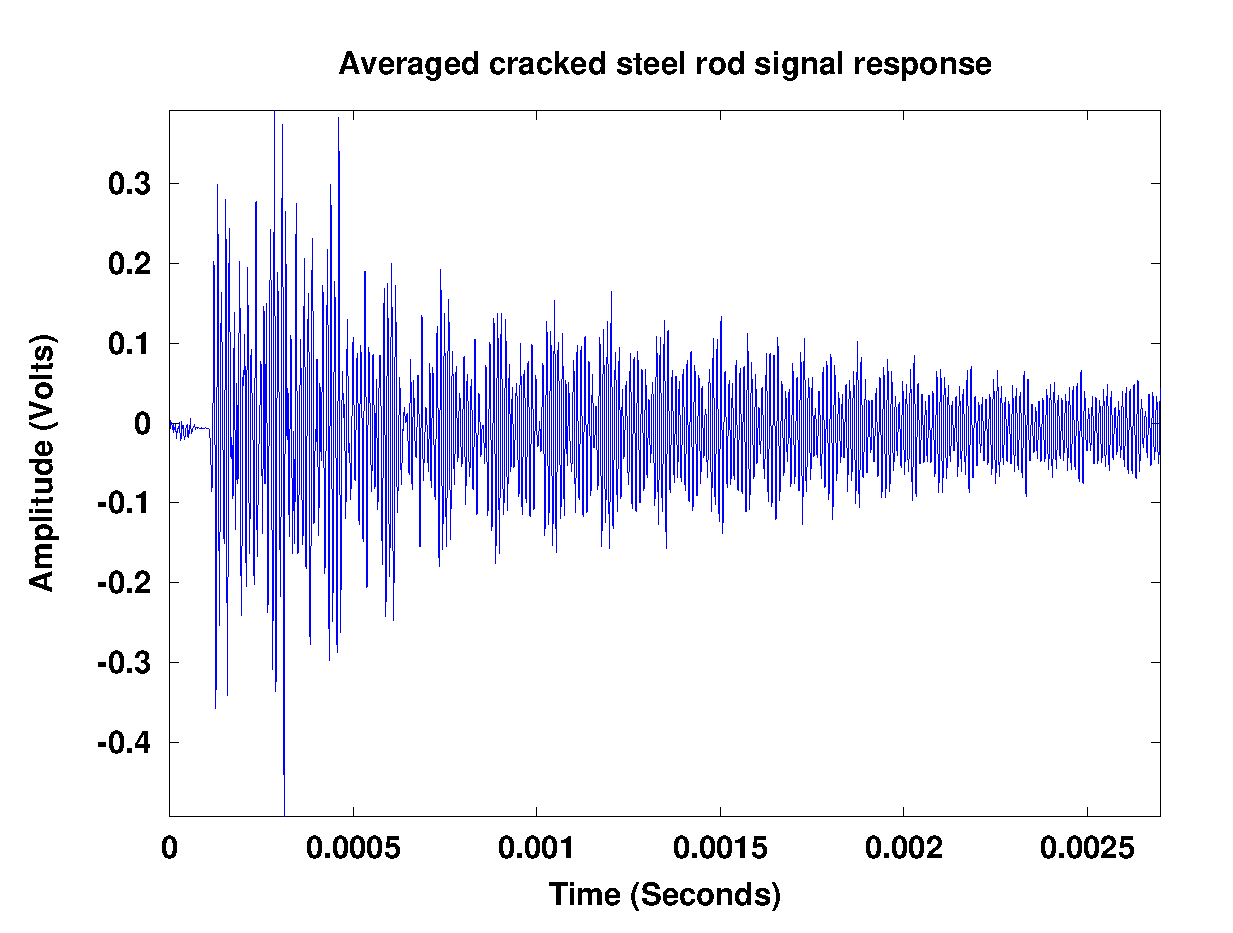
\includegraphics[width=0.6\textwidth]{eps_pics/steelCracked}}
\end{subfigmatrix}

  \caption
%>>>> use \label inside caption to get Fig. number with \ref{}
  { \label{fig:steelCrackResults}
(a) Signal recorded at PZT B with an undamaged steel rod;
(b) Signal recorded at PZT B when using the damaged nylon rod which was represented by using two rod segments whose combined length was equal to that of the undamaged rod.
}
\end{figure}

\begin{figure}[ht!]
\centering
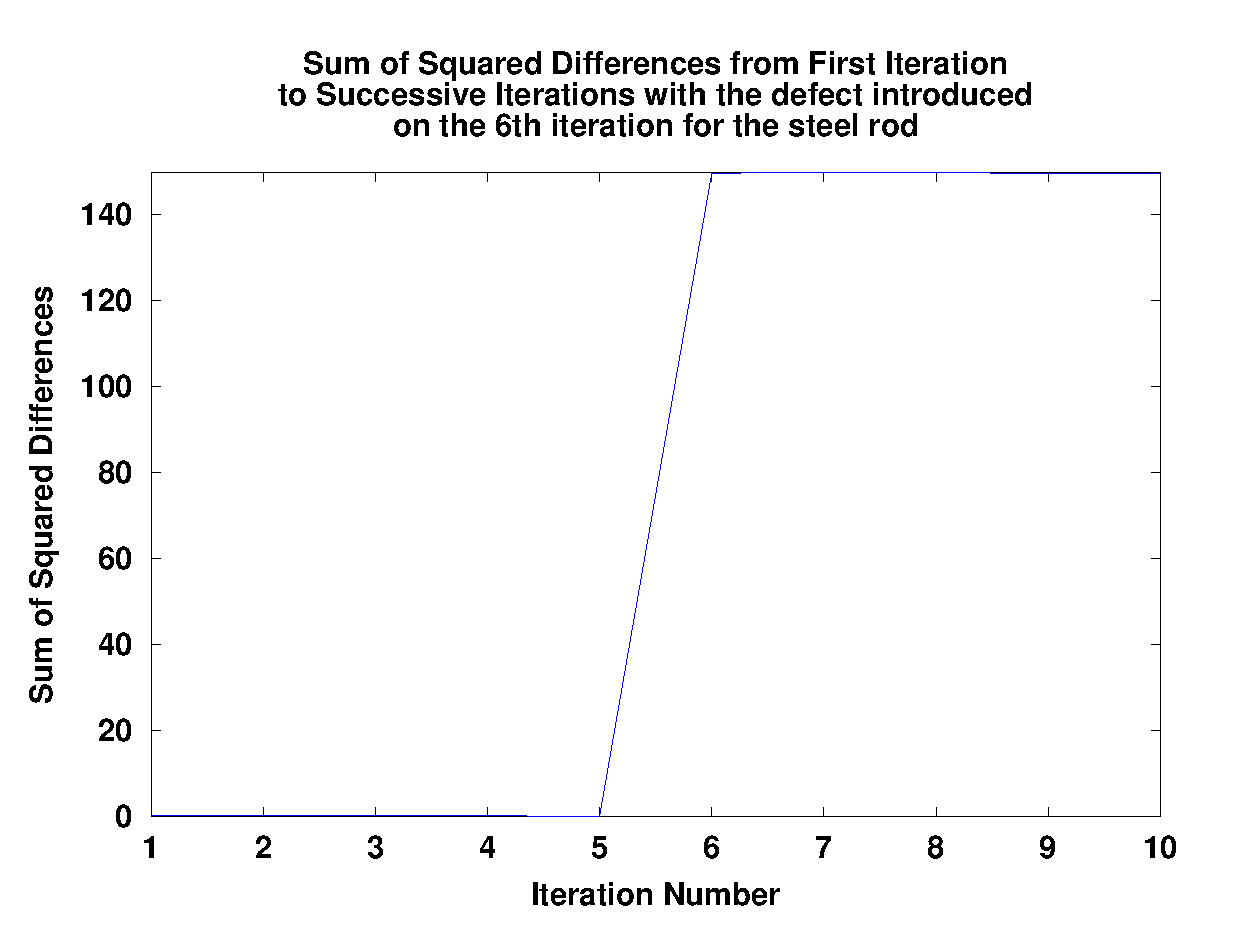
\includegraphics[width=0.6\textwidth]{eps_pics/steelDifferences}
\caption{Sum of squared differences computed for each iteration of the steel rod crack detection tests. The damaged rod was introduced on the 6th iteration and this was clearly seen in the graph data.
 	 \label{fig:steelDifferences}} 
\end{figure}

The same tests were performed using nylon rods. Figure \ref{fig:nylonCrackResults} shows the graphs for both the undamaged and damaged nylon rod crack detection tests. As with the steel rods, a large change in amplitude is seen from the undamaged to the damaged signals. Figure \ref{fig:nylonDifferences} shows the sum of squared differences for each iteration of the nylon rod tests with the damaged rod again being introduced on the 6th iteration. Just as with the steel rods a large jump in the graph is seen when the damaged rod is introduced.

\begin{figure}[ht!]
\begin{subfigmatrix}{2}
\subfigure[PZT B Signal Undamaged Nylon Rod]
{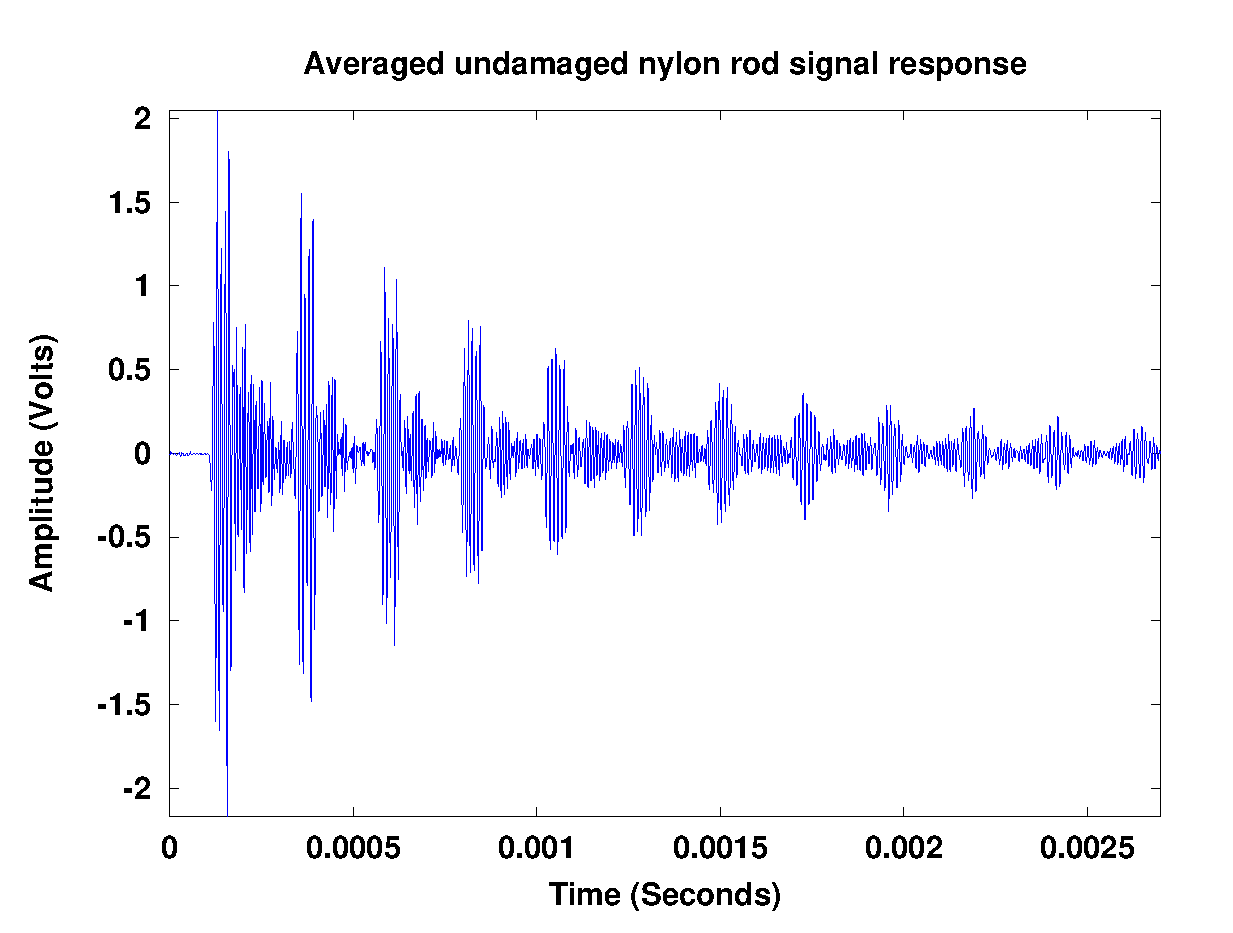
\includegraphics[width=0.6\textwidth]{eps_pics/nylonUncracked}}
\subfigure[PZT B Signal Damaged Nylon Rod]
{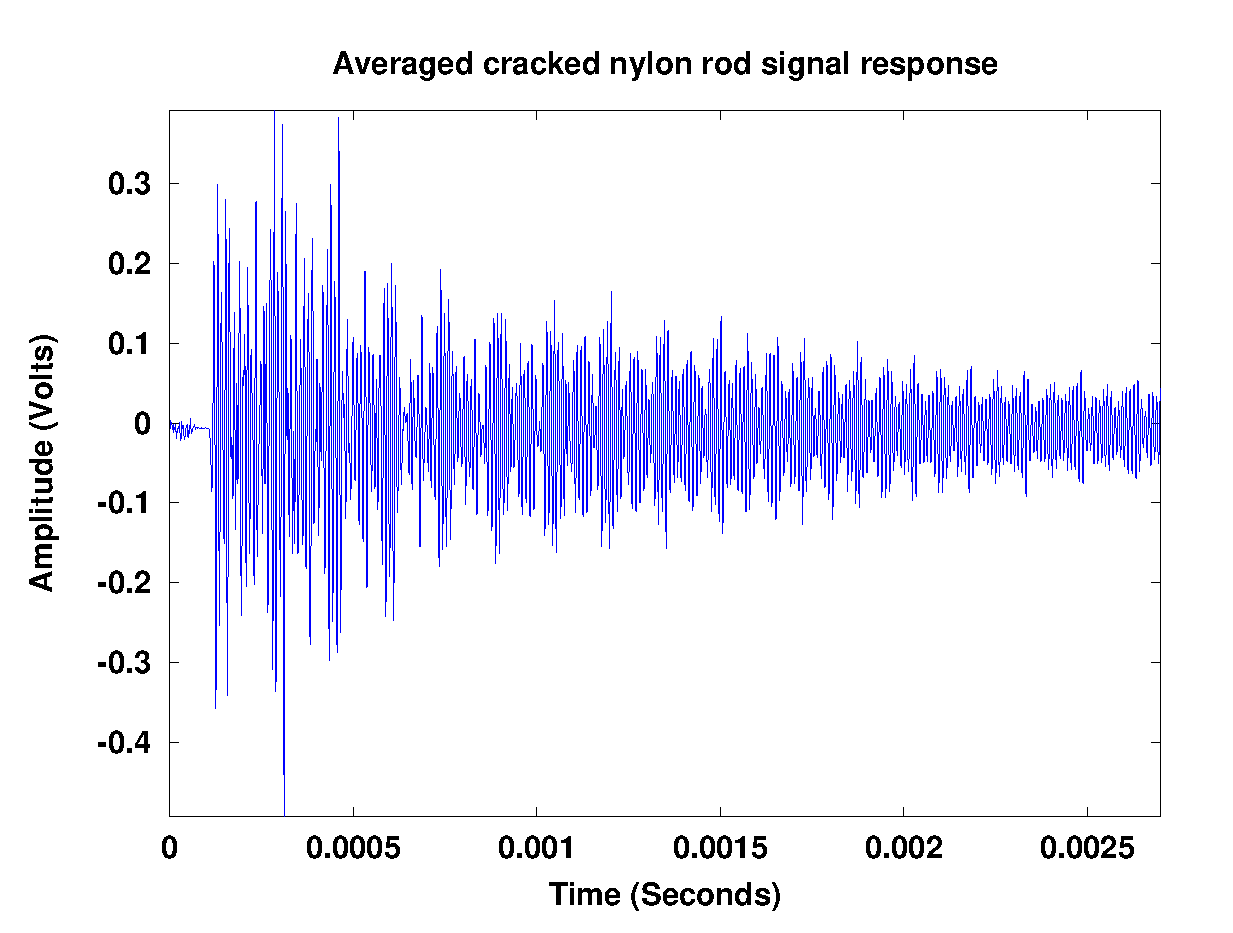
\includegraphics[width=0.6\textwidth]{eps_pics/nylonCracked}}
\end{subfigmatrix}

  \caption
%>>>> use \label inside caption to get Fig. number with \ref{}
  { \label{fig:nylonCrackResults}
(a) Signal recorded at PZT B with an undamaged nylon rod;
(b) Signal recorded at PZT B when using the damaged nylon rod which was represented by using two rod segments whose combined length was equal to that of the undamaged rod.
}
\end{figure}

\begin{figure}[ht!]
\centering
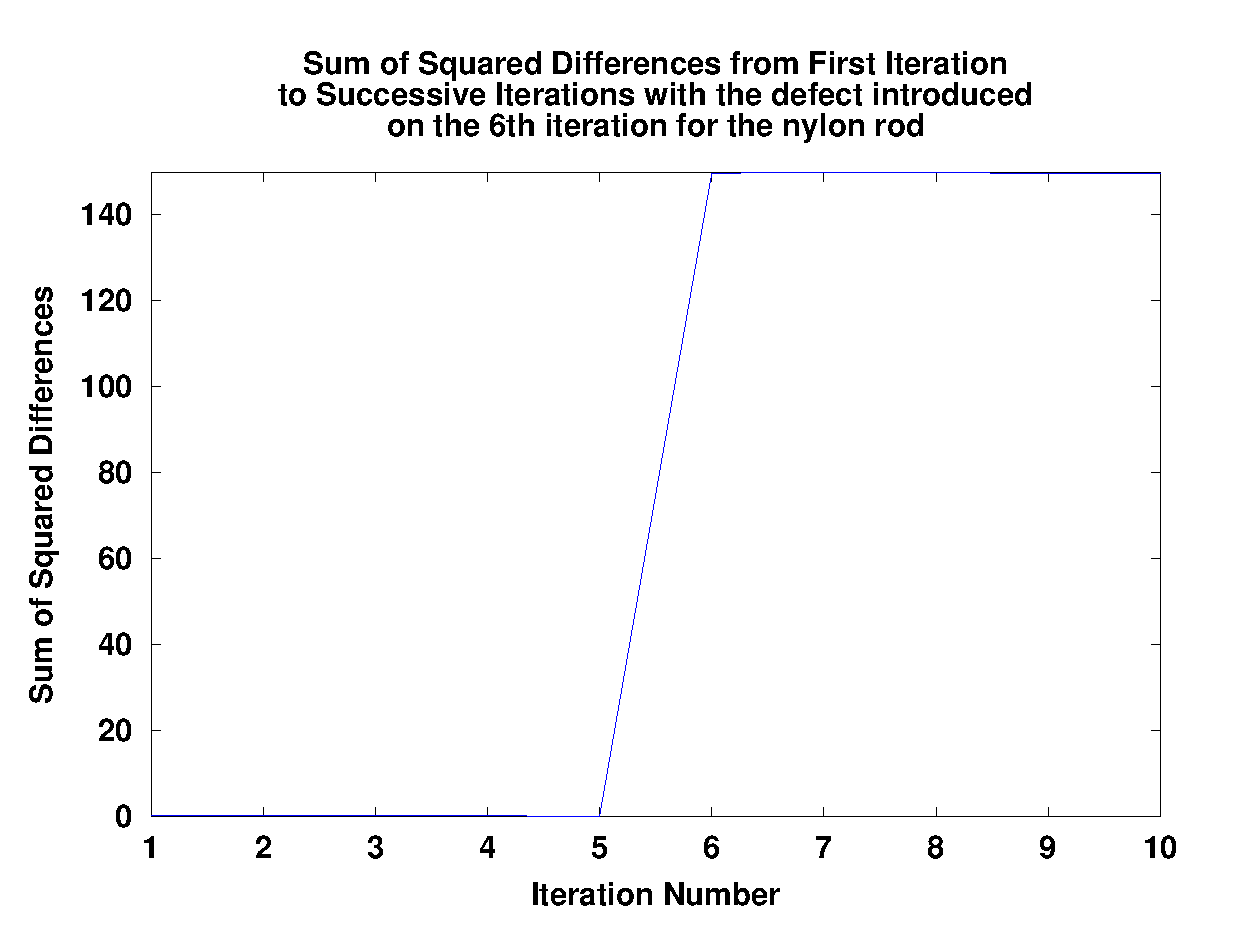
\includegraphics[width=0.6\textwidth]{eps_pics/nylonDifferences}
\caption{Sum of squared differences computed for each iteration of the nylon rod crack detection tests. The damaged rod was introduced on the 6th iteration and, as with the steel rod tests, this is clearly seen in the graph data.
 	 \label{fig:nylonDifferences}} 
\end{figure}

\section{Single Iteration Time Reversal Results}

\subsection{Steel Rods Single Iteration Results}
Theoretical calculations were carried out for the first iteration of the one dimensional time reversal focusing algorithm using the equations described in the modeling section of this thesis. Time reversal focusing was desired to be at the 'defect' PZT with a multi-tone signal over the frequency range of $100 kHz$ - $130 kHz$. The calculations were carried out assuming that there was zero dissipation. Figures \ref{fig:steelThExp1} - \ref{fig:steelThExp3} show the theoretical and experimental results together for each of the three steel rod combinations that were tested. A reasonable match between the results is seen but differences arise due to the calculations not accounting for dispersion or dissipation. The amplitude of the experimental waves are seen to have lower amplitude and an altered shape from the waves seen in the theoretical results. The wave recorded in the time reversal phase was seen to be larger than the response recorded in the interrogatory phase and was the desired result as this implied a focusing of the energy from each wave at the defect location.

\begin{figure}[ht!]
\centering
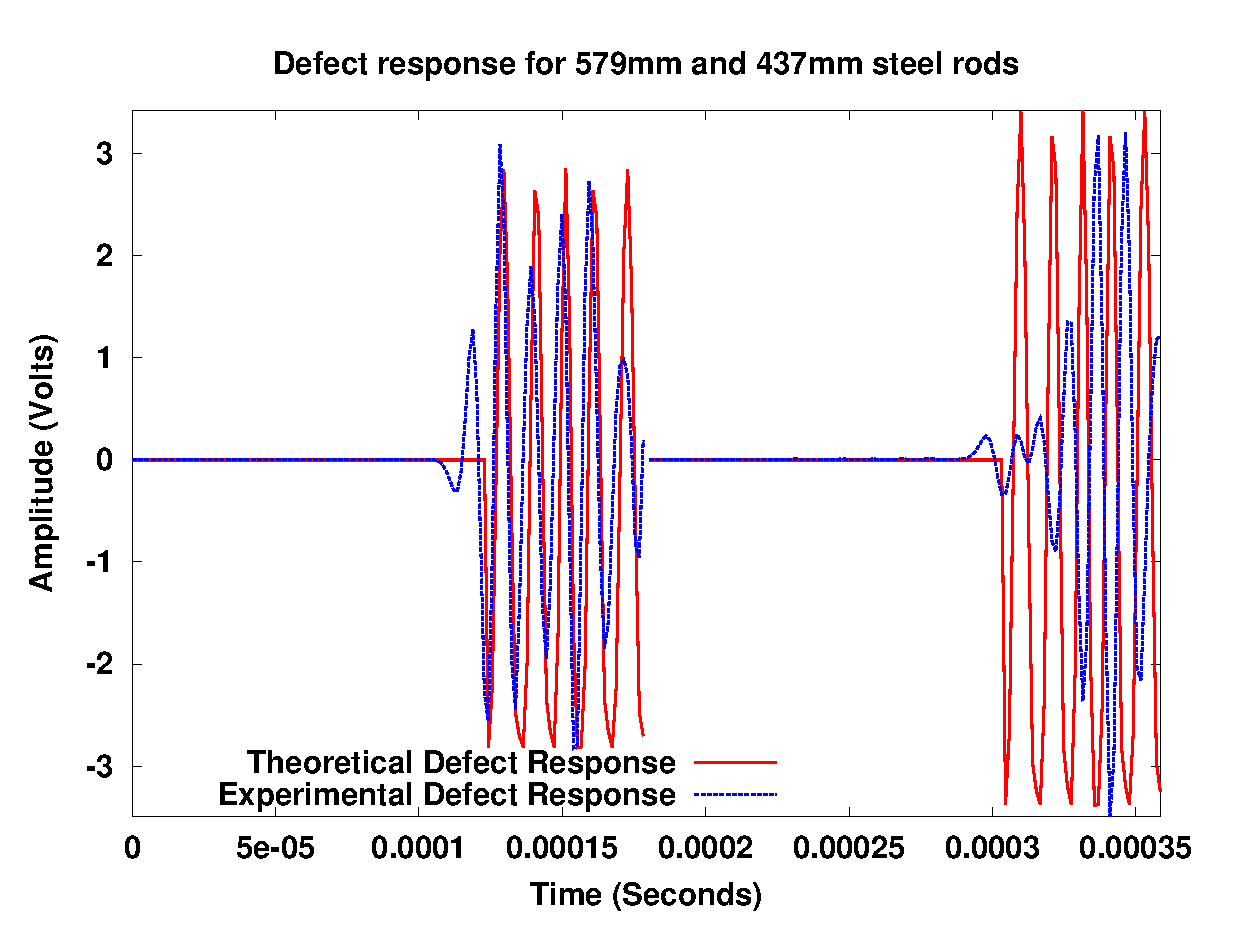
\includegraphics[width=0.6\textwidth]{eps_pics/steel-1-2_Iter_th_exp.eps}
\caption{Theory vs Experiment, $579 mm$ and $437 mm$ steel rods
	 \label{fig:steelThExp1}} 
\end{figure}

\begin{figure}[ht!]
\centering
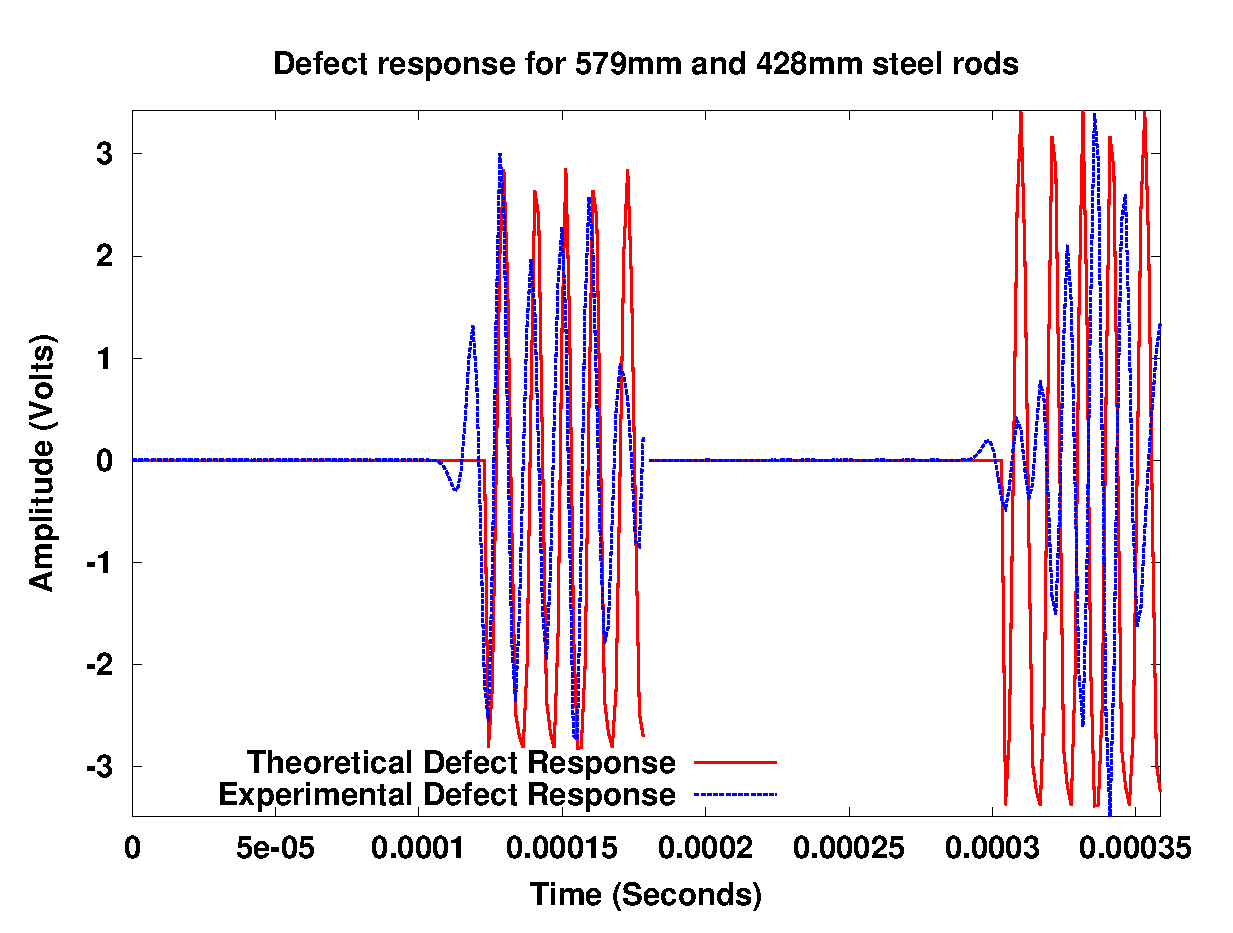
\includegraphics[width=0.6\textwidth]{eps_pics/steel-1-3_Iter_th_exp.eps}
\caption{Theory vs Experiment, $579 mm$ and $428 mm$ steel rods
	 \label{fig:steelThExp2}} 
\end{figure}

\begin{figure}[ht!]
\centering
\includegraphics[width=0.6\textwidth]{eps_pics/steel-2-3_Iter_th_exp.eps}
\caption{Theory vs Experiment, $437 mm$ and $428 mm$ steel rods
	 \label{fig:steelThExp3}} 
\end{figure}

 \subsection{Nylon Rods Single Iteration Results}
 Calculations were also carried out for the nylon rods which was also based upon the models seen previously in this paper. The calculations for the nylon rods also ignored dispersion and dissipation. As with the steel rods, these theoretical results were compared with the experimental results and this comparison is shown for each of the three nylon rod tests Figures \ref{fig:nylonThExp1} - \ref{fig:nylonThExp3}. A worse match is seen in these experiments and is perhaps due to greater dispersion and dissipation within the nylon rods than seen in the steel rods. The overall result was still good though because the wave in the time reversal phase wass again seen to be larger than the wave recorded in the interrogatory phase. This increase in amplitude showed that focusing occurred with the nylon rod tests. 
 
 \begin{figure}[ht!]
 \centering
 \includegraphics[width=0.6\textwidth]{eps_pics/nylon-2-3_Iter_th_exp.eps}
 \caption{Theory vs Experiment, $148 mm$ and $105 mm$ nylon rods
 	 \label{fig:nylonThExp1}} 
 \end{figure}
 
 \begin{figure}[ht!]
 \centering
 \includegraphics[width=0.6\textwidth]{eps_pics/nylon-2-4_Iter_th_exp.eps}
 \caption{Theory vs Experiment, $148 mm$ and $75 mm$ nylon rods
 	 \label{fig:nylonThExp2}} 
 \end{figure}
 
 \begin{figure}[ht!]
 \centering
 \includegraphics[width=0.6\textwidth]{eps_pics/nylon-3-4_Iter_th_exp.eps}
 \caption{Theory vs Experiment, $105 mm$ and $75 mm$ nylon rods
 	 \label{fig:nylonThExp3}} 
 \end{figure}
 
 
 \section{Iterative Time Reversal Results}
 The time reversal algorithm was applied iteratively in both the steel and nylon rod tests. The goal of the iterative reversal was to see an increase in the response amplitude at the defect with each iteration. For each iteration the amplitude gain at the defect was recorded and used to determine the overall effectiveness of applying the time  reversal algorithm in an iterative fashion. The gain was determined by comparing the max peak to peak amplitude recorded at the defect on each iteration with the max response recorded on the first iteration. The max peak to peak amplitude was taken to be $|max(DefectVoltage) - min(DefectVOltage)|$. The gain was then computed as $CurrentMax / InitialMax$ and this was plotted for each time reversal iteration. 
 
 \subsection{Steel Rods Multiple Iteration Results}
 For the steel rod tests it was seen that the amplitude of the gain increased rapidly in the beginning of the experiments as the algorithm found a better and better signal with each iteration for the PZTs to playback. The gain began to level off as the number of iterations increased and the algorithm started to converge on a playback signal for each PZT. In the gain plots for the three steel rod tests it is seen that the gain increased substantially in the beginning and then leveled out (Figures \ref{fig:steelIter1} - \ref{fig:steelIter3}). It was noticed that the final gain seen may not necessarily have been the maximum gain achieved throughout the iterative process. This suggests that further refinements could be made to the time reversal algorithm such that the optimal playback waves would be found, and also suggests that more descriptive models are needed to further understand the underlying principles of time reversal.

\begin{figure}[ht!]
\centering
\includegraphics[width=0.6\textwidth]{eps_pics/steel-1-2_iterationVsGain.eps}
\caption{Amplitude gain at the defect on each iteration for the $579 mm$ and $437 mm$ steel rod iterative time reversal test with a final gain of a little over 2. The gain did not appear to completely level out, but it slowly oscillated right around 2.
	 \label{fig:steelIter1}} 
\end{figure}
  
\begin{figure}[ht!]
\centering
\includegraphics[width=0.6\textwidth]{eps_pics/steel-1-3_iterationVsGain.eps}
\caption{Defect amplitude gain on each iteration for the $579 mm$ and $428 mm$ steel rod iterative time reversal test with a final gain of a little over 2.5.
 	 \label{fig:steelIter2}} 
\end{figure}

\begin{figure}[ht!]
\centering
\includegraphics[width=0.6\textwidth]{eps_pics/steel-2-3_iterationVsGain.eps}
\caption{Defect amplitude gain on each iteration for the $437 mm$ and $428 mm$ steel rod iterative time reversal test with a final gain of about 3.
  	 \label{fig:steelIter3}} 
\end{figure}

 
 The other method used to gauge the performance of the iterative time reversal was to compare the signature of the response at the defect on both the first and last iteration. If the algorithm worked correctly then what should have been seen is that the final wave was purer and of larger amplitude than the initial wave. This is in fact what was seen in the steel rod tests. The comparison of the first and initial waves at the defect are shown for each of the three steel rod tests in Figures \ref{fig:steelExp1} - \ref{fig:steelExp3}.
 
  \begin{figure}
 \begin{subfigmatrix}{2}
 \subfigure[Defect Response Initial Iteration, $579 mm$ and $437 mm$ steel rods]
 {\includegraphics[width=0.6\textwidth]{eps_pics/steel-1-2_Initial.eps}}
 \subfigure[Defect Response 150th Iteration, $579 mm$ and $437 mm$ steel rods]
 {\includegraphics[width=0.6\textwidth]{eps_pics/steel-1-2_Final.eps}}
 \end{subfigmatrix}
 
    \caption
 %>>>> use \label inside caption to get Fig. number with \ref{}
    { \label{fig:steelExp1}
    a) First wave seen at the defect on the initial iteration for the $579 mm$ and $437 mm$ steel rod test.; b) Wave recorded at the defect after 150 iterations. The wave was much more defined and more than doubled in amplitude since the first iteration.
  }
 \end{figure}
 
  \begin{figure}
 \begin{subfigmatrix}{2}
 \subfigure[Defect Response Initial Iteration, $579 mm$ and $428 mm$ steel rods]
 {\includegraphics[width=0.6\textwidth]{eps_pics/steel-1-3_Initial.eps}}
 \subfigure[Defect Response 150th Iteration, $579 mm$ and $428 mm$ steel rods]
 {\includegraphics[width=0.6\textwidth]{eps_pics/steel-1-3_Final.eps}}
 \end{subfigmatrix}
 
    \caption
 %>>>> use \label inside caption to get Fig. number with \ref{}
    { \label{fig:steelExp2}
    a) First wave seen at the defect on the initial iteration for the $579 mm$ and $428 mm$ steel rod test.; b) Wave recorded at the defect after 150 iterations. Like the $579 mm$ and $437 mm$ steel rod results, this wave was much more defined and more than doubled in amplitude since the first iteration.
  }
 \end{figure}
 
  \begin{figure}
 \begin{subfigmatrix}{2}
 \subfigure[Defect Response Initial Iteration, $437 mm$ and $428 mm$ steel rods]
 {\includegraphics[width=0.6\textwidth]{eps_pics/steel-2-3_Initial.eps}}
 \subfigure[Defect Response 150th Iteration, $437 mm$ and $428 mm$ steel rods]
 {\includegraphics[width=0.6\textwidth]{eps_pics/steel-2-3_Final.eps}}
 \end{subfigmatrix}
 
    \caption
 %>>>> use \label inside caption to get Fig. number with \ref{}
    { \label{fig:steelExp3}
    a) First wave seen at the defect on the initial iteration for the $437 mm$ and $428 mm$ steel rod test.; b) Wave recorded at the defect after 150 iterations. The amplitude of the wave nearly tripled since the first iteration.
  }
 \end{figure}
 
 \subsection{Nylon Rods Multiple Iteration Results}
 As with the steel rod tests, the amplitude gain seen at the defect on each iteration was plotted for the three nylon rod tests (Figures \ref{fig:nylonIter1} - \ref{fig:nylonIter2}). With the nylon rods an even higher gain was seen than with the steel rod tests. The nylon tests showed an average gain of over 3 whereas the gains seen with the steel rod tests were closer to 2. The first and final waves recorded at the defect are also compared for each of the nylon tests and these results are shown in Figures \ref{fig:nylonExp1} - \ref{fig:nylonExp3}. It was seen that final wave was of much greater amplitude than the initial wave for all of the tests performed.
 
 \begin{figure}[ht!]
 \centering
 \includegraphics[width=0.6\textwidth]{eps_pics/nylon-2-3_iterationVsGain.eps}
 \caption{Defect amplitude gain that was achieved at the defect for each iteration of the time reversal algorithm for the $148 mm$ and $105 mm$ nylon rods. The gain leveled out around 3.
 	 \label{fig:nylonIter1}} 
 \end{figure}
   
 \begin{figure}[ht!]
 \centering
 \includegraphics[width=0.6\textwidth]{eps_pics/nylon-2-4_iterationVsGain.eps}
 \caption{Defect amplitude gain that was achieved at the defect for each iteration of the time reversal algorithm for the $148 mm$ and $75 mm$ nylon rods. The final gain of a little over 3 was reached by about the 25th iteration as seen in other tests.
  	 \label{fig:nylonIter2}} 
 \end{figure}
 
 \begin{figure}[ht!]
 \centering
 \includegraphics[width=0.6\textwidth]{eps_pics/nylon-3-4_iterationVsGain.eps}
 \caption{Defect amplitude gain that was achieved at the defect for each iteration of the time reversal algorithm for the $105 mm$ and $75 mm$ nylon rods. The final gain seen was about 2.75. This test was a good example of the final gain being lower than the max gain that was seen and suggests that the algorithm could be further improved.
  	 \label{fig:nylonIter3}} 
 \end{figure}
 
 
  \begin{figure}
 \begin{subfigmatrix}{2}
 \subfigure[Defect Response Initial Iteration, $148 mm$ and $105 mm$ nylon rods]
 {\includegraphics[width=0.6\textwidth]{eps_pics/nylon-2-3_Initial.eps}}
 \subfigure[Defect Response 150th Iteration, $148 mm$ and $105 mm$ nylon rods]
 {\includegraphics[width=0.6\textwidth]{eps_pics/nylon-2-3_Final.eps}}
 \end{subfigmatrix}
 
    \caption
 %>>>> use \label inside caption to get Fig. number with \ref{}
    { \label{fig:nylonExp1}
    a) First wave seen at the defect on the initial iteration for the $148 mm$ and $105 mm$ nylon rod test.; b) Wave recorded at the defect after 150 iterations. The final wave more than tripled in amplitude from the first wave.
  }
 \end{figure}
 
  \begin{figure}
 \begin{subfigmatrix}{2}
 \subfigure[Defect Response Initial Iteration, $148 mm$ and $75 mm$ nylon rods]
 {\includegraphics[width=0.6\textwidth]{eps_pics/nylon-2-4_Initial.eps}}
 \subfigure[Defect Response 150th Iteration, $148 mm$ and $75 mm$ nylon rods]
 {\includegraphics[width=0.6\textwidth]{eps_pics/nylon-2-4_Final.eps}}
 \end{subfigmatrix}

    \caption
 %>>>> use \label inside caption to get Fig. number with \ref{}
    { \label{fig:nylonExp2}
    a) First wave seen at the defect on the initial iteration for the $148 mm$ and $75 mm$ nylon rod test.; b) Wave recorded at the defect after 150 iterations. Again, the response seen at the defect has tripled.
  }
 \end{figure}
 
  \begin{figure}
 \begin{subfigmatrix}{2}
 \subfigure[Defect Response Initial Iteration, $105 mm$ and $75 mm$ nylon rods]
 {\includegraphics[width=0.6\textwidth]{eps_pics/nylon-3-4_Initial.eps}}
 \subfigure[Defect Response 150th Iteration, $105 mm$ and $75 mm$ nylon rods]
 {\includegraphics[width=0.6\textwidth]{eps_pics/nylon-3-4_Final.eps}}
 \end{subfigmatrix}
 
    \caption
 %>>>> use \label inside caption to get Fig. number with \ref{}
    { \label{fig:nylonExp3}
    a) First wave seen at the defect on the initial iteration for the $105 mm$ and $75 mm$ nylon rod test.; b) Wave recorded at the defect after 150 iterations.
  }
 \end{figure}
 

%\chapter{Recommended Future Work}\label{ch:RecommendedFutureWork}
%%recommended work


\chapter{Conclusion}\label{ch:Conclusion}
% A conclusion chapter

The motivation of this work was to accelerate the recovery rate of a self healing polymer by focusing acoustic energy at the recovery site. Time reversal signal processing was the algorithm chosen to achieve the localized pressure at an arbitrarily positioned crack whose location was unknown. In this work one-dimensional time reversal was explored both theoretically and experimentally, with the novelty being experimental verification that time reversal is achievable in a one-dimensional system such as a finite length rod. The first step was to determine if it was possible to detect when damage had occurred within the rod. The crack detection tests showed that there was large change in the wave signature of a stress wave sent from one end of the rod and recorded the other when a crack was introduced. The change in wave signature could easily be detected in software to signal the start of the time reversal process. Next, calculations were performed using models derived by Dr. Umesh Korde for both the steel and nylon rod cases \cite{Fehrman2012}. Rod segments of random lengths were used and a PZT sandwiched between the segments acted as the defect location. The theoretical models were compared with the experimental models and a decent match was seen. The difference between the theory and experiments could be due to the model not taking in to account dispersion, dissipation, PZT ringing, and other physical phenomena. Still, it was seen that the amplitude of the response at the defect location increased by using time reversal. Lastly, iterative time reversal was performed to see if the stress wave energy at the crack location would increase with successive iterations until the algorithm converged on the playback signals used in the time reversal phase. The experiments showed that the amplitude gain increased rapidly in the beginning of the time reversal process and then began to level out. The nylon rods proved to have better results than the steel rods and this was consistent with previously published work \cite{Fink1993}. 

Future work will involve modeling which includes more real life phenomena such as the transducer ringer, dispersion, dissipation, and other variables which change the shape, amplitude, phase, and other characteristics of the propagated wave. The time reversal testing should also be performed on a self healing polymer to determine if the method can in fact increase the recovery rate at a healing site.


\bibliographystyle{unsrt}
\bibliography{thesis}

\setcounter{secnumdepth}{0}
\chapter*{Code Appendix}
\addcontentsline{toc}{chapter}{Code Appendix}
%Appendix
\section{Crack Detection Matlab Plot Code}

\begin{lstlisting}
function []= crack_plot(foldernameUncracked, foldernameCracked)

%Set font size
font_s = 15;

%Set time step
time_step = 54/40000000;

%Load each uncracked result
for(i = 0:4)
filename = strcat(foldernameUncracked,  num2str(i), 
'_Signals', '.lvm');
uncracked(i+1,:,:) = load(filename);
	
%Load each cracked result	
filename = strcat(foldernameCracked,  num2str(i), 
'_Signals', '.lvm');
cracked(i+1,:,:) = load(filename);
end

%Find the sum of squared differences between first signal
%and the next 4 signals
for(i = 1:4)
difference(i) = 0;
	for(j = 1:size(cracked)(2))
	unsquared = uncracked(1,j,2) - uncracked(i+1,j,2) ;
	difference(i) = difference(i) + unsquared^2;
	end
end

%Find the sum of squared differences between first signal
%and the last 5 signals
for(i = 1:5)
difference(i+5) = 0;
	for(j = 1:size(cracked)(2))
	unsquared = uncracked(1,j,2) - cracked(i,j,2) ;
	difference(i+5) = difference(i+5) + unsquared^2;
	end
end
%Plot the difference array and set plot parameters
figure(1)
plot(difference)

axis tight
xlabel('Iteration Number', 'FontSize', font_s, 'FontWeight', 'bold')
ylabel('Sum of Squared Differences', 'FontSize', font_s,
 'FontWeight', 'bold')
set(gca, 'FontSize', font_s, 'FontWeight', 'bold')
title({'Sum of Squared Differences from First Iteration',
'to Successive Iterations with the defect introduced', 
'on the 6th iteration for the steel rod'}, 
'FontSize', font_s, 'FontWeight', 'bold')
print('-depsc', 'steelDifferences');

//Average 5 uncracked runs and 5 cracked runs
uncrackedAvg = sum(uncracked) / 5;
crackedAvg = sum(cracked) / 5;

t = 0:time_step:time_step * length(uncrackedAvg) - time_step;

%Plot the averaged uncracked and cracked results
figure(2)
plot(t,uncrackedAvg(1,:,2))

axis tight
xlabel('Time (Seconds)', 'FontSize', font_s, 'FontWeight', 'bold')
ylabel('Amplitude (Volts)', 'FontSize', font_s, 
'FontWeight', 'bold')
set(gca, 'FontSize', font_s, 'FontWeight', 'bold')
title({'Averaged undamaged steel rod signal response'},
'FontSize', font_s, 'FontWeight', 'bold')
print('-depsc', 'steelUncracked');

figure(3)
plot(t,crackedAvg(1,:,2))

axis tight
xlabel('Time (Seconds)', 'FontSize', font_s, 'FontWeight', 'bold')
ylabel('Amplitude (Volts)', 'FontSize', font_s, 
'FontWeight', 'bold')
set(gca, 'FontSize', font_s, 'FontWeight', 'bold')
title({'Averaged cracked steel rod signal response'}, 
'FontSize', font_s, 'FontWeight', 'bold')
print('-depsc', 'steelCracked');

\end{lstlisting}

\section{Time Reversal Results Matlab Plot Code}

\begin{lstlisting}
%Originally written by Dr. Korde, modified and appended
%by Brian Fehrman

%Clean slate
close all
clear all

%Load the wave that was initially sent
wave = load('initialWave.lvm');

%Set the basename for file opens/saves
basename = "steel-2-3_"

%Set the font size
font_s = 15;

%Get the correct time array for plotting
time_step = 54/40000000;

%Create time array for plotting
t_wave = 0:time_step:time_step * length(wave) - time_step;

%Plot initial wave
figure_count= 1;
figure(figure_count)
plot(t_wave, wave)
title('Wave used')
xlabel('Time (seconds)')
ylabel('Amplitude (volts)')
figure_count = figure_count + 1;


%Taking speed of sound in structural steel to be 4623 m/s and
%sample speed of FPGA to be 1.35e-6, determine time taken for
%the wave to reach the defect location
speed_sound = 4623;
l_rod = .437;
sample_speed = 1.35e-6;
travel_time = l_rod / speed_sound;
num_samples = travel_time / sample_speed;

%Wave sent
chirpin = [zeros(num_samples, 1)' wave(:,1)'];

%Get correct size time array for plotting
N = num_samples + length(wave);
t_theory = 0:time_step:time_step * N - time_step;

% Steel rod and piezo parameters
eps0 = 8.854e-12; eps33 = 450*eps0; d33 = 152.0e-12; c33 = 11.3e10;
R0 = 1e2; RL = R0; rho = 7.6e3; 
rhost = 7.894e3;c33st = 16.939e10; a = 19.05e-3;
a = 12.7e-3; l = 12e-3; L = 437e-3;
lc = L; lT = 310e-3;

% M magnification applied in play-back
% M be set as the reciprocal of the maximum 
%voltage of the reversed impulse response
M = 10; 

% Voltage V0
V0 = 20.0;
c = sqrt(c33/rho); cst = sqrt(c33st/rhost);
s33 = 1/c33; s33st = 1/c33st;


% Effect of crack is a localized change in c33st and rhost.
c33stc = 0.9*c33st;
rhostc = 0.9*rhost;

%Terms in constitutive relations
d3 = 1 - d33^2/(s33*eps33);
c33bar = 1/(s33*d3);
d33bar = (-d33/eps33)/d3;
eps33bar = eps33/d3;
area = pi*a^2;
Cc = eps33bar*area/l;
alpha = 1/(RL*Cc);
Rterm1 = c33bar + (d33bar*d33)/(2*s33);
Rterm2 = c33st;

% R reflection coefficient
R = (Rterm1 - Rterm2)/(Rterm1 + Rterm2);
Rc = (c33st - c33stc)/(c33st + c33stc);
Rhat = (Rterm2-Rterm1)/(Rterm1+Rterm2);

%T reflection coefficient
T = 1-abs(R);
Tc = 1-abs(Rc);
That = 1 - abs(Rhat);

%Actuator amplitude coefficient
wactamp = abs(T)*(1+abs(T)*abs(That)*M/RL/Cc);

%Crack amplitude coefficient
wcrackamp = abs(T)*(abs(T)*abs(That)*M/RL/Cc)*(Rc+Tc);

%Determine response at the crack location
deltt = 54/40e6;
delt = deltt;
chirprevcrack = zeros(N,1);
vlongchirp = zeros(N,1);

for i = 1:N;
    t(i) = (i-1)*deltt;
    wcrack(i) = wcrackamp*exp(-t(i)*alpha);
end


for k = 1:N;
    sum = 0;
    for i = 1:k;
        sum = sum + wcrack(i)*chirpin(k-i+1)*delt;
    end
    chirprevcrack(k) = sum;
end
%
Pamp = (d33*area*RL)/(2*s33);
amp = 1.0e-2; %scaling for transducer

%Response at crack on first iteration
vlongchirp1 = Pamp*amp*chirprevcrack;

%Repsponse at crack on second iteration
vlongchirp2 = Pamp*amp*chirprevcrack * 1.2;

%Number of iteration samples to look at.
% There are 6 total available
num_iterations = 2;

defect = [];

%Load the data from each iteration
    
temp = load( '0_Signals.lvm');
temp2 = temp(:,3);
defect(:,1) = temp2(1:N);

temp = load( '1_Signals.lvm');
temp2 = temp(:,3);
defect(:,2) = temp2(1:N);


defect_avg = 0;

avg_start = 1;

%Get average value of end of signals. 
%Used for trying to center signals around zero
for i = avg_start:N
   defect_avg = defect_avg + defect(i,1);
end

defect_avg = defect_avg / (N - avg_start);

%Subtract the average value of each signal from
%the signal. This attempts to center each signal 
%around zero since the voltage readings aren't
%centered around zero.
for i = 1:num_iterations
    defect(:,i) = defect(:,i) - defect_avg; 
end

defect_cat = [];

for i = 1:num_iterations
  defect_cat = [defect_cat defect(:,i)'];
end

theory_cat = [vlongchirp1(:,1)' vlongchirp2(:,1)'];

t_theory_cat = 0:time_step:time_step * 
length(theory_cat) - time_step;

figure(figure_count)
plot(t_theory, vlongchirp1, t_theory, defect(:, 1))
title({'Theoretical and Experimental Defect Response Superimposed', 
'(Initial Phase)'})
xlabel('Time (seconds)')
ylabel('Amplitude (volts)')
legend('Theoretical Defect Response', 'Experimental Defect Response')
figure_count = figure_count + 1;

figure(figure_count)
plot(t_theory, vlongchirp2, t_theory, defect(:, 2))
title({'Theoretical and Experimental Defect Response Superimposed', 
'(Time Reversal Phase {First Iteration})'})
xlabel('Time (seconds)')
ylabel('Amplitude (volts)')
legend('Theoretical Defect Response', 'Experimental Defect Response')
figure_count = figure_count + 1;

figure(figure_count)
plot(t_theory_cat, theory_cat, t_theory_cat, defect_cat)
title({'Theoretical and Experimental Defect Responses Superimposed', 
'Intial Phase and Time Reversal Phase {First Iteration}', 
'(actual time delay between phases not shown due to magnitude)'})
xlabel('Time (seconds)')
ylabel('Amplitude (volts)')
legend('Theoretical Defect Response', 'Experimental Defect Response')
figure_count = figure_count + 1;

%Plot the theory vs experiments
t_theory2 = time_step*N:time_step: 2 * time_step*N - time_step;
figure(figure_count)
plot(t_theory, vlongchirp1,'-r','LineWidth',4, t_theory,
defect(:, 1),'--b','LineWidth',4, t_theory2, vlongchirp2,
'-r','LineWidth',4, t_theory2, defect(:, 2),
'--b','LineWidth',4)
axis tight
xlabel('Time (Seconds)', 'FontSize', font_s, 'FontWeight', 'bold')
ylabel('Amplitude (Volts)', 'FontSize', font_s, 'FontWeight', 'bold')
set(gca, 'FontSize', font_s, 'FontWeight', 'bold')
title('Defect response for 437mm and 428mm steel rods', 
'FontSize', font_s, 'FontWeight', 'bold')
thisLegend = legend('Theoretical Defect Response', 
'Experimental Defect Response',
'Location','SouthWest')
figure_count = figure_count + 1;
set(thisLegend, 'FontSize', font_s, 'FontWeight', 'bold')
print('-depsc',  strcat(basename, 'Iter_th_exp'));

%Plot initial defect response
initial = load(strcat(basename, 'Initial.lvm'));
t = 0:time_step:length(initial) * time_step - time_step;
figure(figure_count)
plot(t, initial,'LineWidth',4)
axis tight
xlabel('Time (Seconds)', 'FontSize', font_s,
 'FontWeight', 'bold')
ylabel('Amplitude (Volts)', 'FontSize', font_s, 'FontWeight', 'bold')
set(gca, 'FontSize', font_s, 'FontWeight', 'bold')
title({'Response at defect PZT on initial iteration for the steel rods', 
'of length 437mm and 428mm'}, 'FontSize', font_s,
 'FontWeight', 'bold')
figure_count = figure_count + 1;
set(thisLegend, 'FontSize', font_s, 'FontWeight', 'bold')
print('-depsc',  strcat(basename, 'Initial'));
final = load(strcat(basename, 'Final.lvm'));

%Plot final defect response
figure(figure_count)
plot(t, final,'LineWidth',4)
axis tight
xlabel('Time (Seconds)', 'FontSize', font_s, 
'FontWeight', 'bold')
ylabel('Amplitude (Volts)', 'FontSize', font_s,
 'FontWeight', 'bold')
set(gca, 'FontSize', font_s, 'FontWeight', 'bold')
title({'Response at defect PZT on the 150th iteration for the steel rods',
 'of length 437mm and 428mm'}, 'FontSize', font_s, 
 'FontWeight', 'bold')
figure_count = figure_count + 1;
set(thisLegend, 'FontSize', font_s, 'FontWeight', 'bold')
print('-depsc',  strcat(basename, 'Final'));

%Gain plot
gain = load(strcat(basename, 'iterationVsGain.lvm'));
figure(figure_count)
plot(gain,'LineWidth',4)
axis tight
xlabel('Iteration Number', 'FontSize', font_s,
 'FontWeight', 'bold')
ylabel('Gain (currentAmp / initialAmp)', 'FontSize', font_s, 
'FontWeight', 'bold')
set(gca, 'FontSize', font_s, 'FontWeight', 'bold')
title({'The amplitude gain of the response seen at the defect on each', 
'iteration for the 437mm and 428mm steel rods'}, 
'FontSize', font_s, 'FontWeight', 'bold')
figure_count = figure_count + 1;
set(thisLegend, 'FontSize', font_s, 'FontWeight', 'bold')
print('-depsc',  strcat(basename, 'iterationVsGain'));

%Plot initial wave sent
initialWave = load('initialWave.lvm');
t = 0:time_step: length(initialWave) * time_step - time_step;
figure(figure_count)
plot(t, initialWave,'LineWidth',4)
axis tight
xlabel('Time (Seconds)', 'FontSize', font_s,
 'FontWeight', 'bold')
ylabel('Amplitude (Volts)', 'FontSize', font_s, 
'FontWeight', 'bold')
set(gca, 'FontSize', font_s, 'FontWeight', 'bold')
title({'Multi-tone wave sent by PZT A on initial iteration', 
'115kHz center frequency with 30kHz bandwidth'}, 
'FontSize', font_s, 'FontWeight', 'bold')
figure_count = figure_count + 1;
set(thisLegend, 'FontSize', font_s, 'FontWeight', 'bold')
print('-depsc', 'initialWave');

%Plot signal read by ch0 on first iteration
ch0Read = load('ch0Read.lvm');
t = 0:time_step: length(ch0Read) * time_step - time_step;
figure(figure_count)
plot(t, ch0Read,'LineWidth',4)
axis tight
xlabel('Time (Seconds)', 'FontSize', font_s, 
'FontWeight', 'bold')
ylabel('Amplitude (Volts)', 'FontSize', font_s, 
'FontWeight', 'bold')
set(gca, 'FontSize', font_s, 'FontWeight', 'bold')
title({'Signal read by PZT A on the initial iteration'},
 'FontSize', font_s, 'FontWeight', 'bold')
figure_count = figure_count + 1;
set(thisLegend, 'FontSize', font_s, 'FontWeight', 'bold')
print('-depsc',   'ch0Read');

%Plot signal read by ch1 on first iteration
ch1Read = load('ch1Read.lvm');
t = 0:time_step: length(ch1Read) * time_step - time_step;
figure(figure_count)
plot(t,ch1Read,'LineWidth',4)
axis tight
xlabel('Time (Seconds)', 'FontSize', font_s, 
'FontWeight', 'bold')
ylabel('Amplitude (Volts)', 'FontSize', font_s, 
'FontWeight', 'bold')
set(gca, 'FontSize', font_s, 'FontWeight', 'bold')
title({'Signal read by PZT B on the initial iteration'}, 
'FontSize', font_s, 'FontWeight', 'bold')
figure_count = figure_count + 1;
set(thisLegend, 'FontSize', font_s, 'FontWeight', 'bold')
print('-depsc', 'ch1Read');

%Plot windowed RMS of signal read by ch0 on first iteration
ch0RMS = load('ch0RMS.lvm');
t = 0:time_step: length(ch0RMS) * time_step - time_step;
figure(figure_count)
plot(t,ch0RMS,'LineWidth',4)
axis tight
xlabel('Time (Seconds)', 'FontSize', font_s, 
'FontWeight', 'bold')
ylabel('Amplitude (Volts)', 'FontSize', font_s,
 'FontWeight', 'bold')
set(gca, 'FontSize', font_s, 'FontWeight', 'bold')
title({'Windowed RMS of signal read by PZT A on the initial iteration'},
 'FontSize', font_s, 'FontWeight', 'bold')
figure_count = figure_count + 1;
set(thisLegend, 'FontSize', font_s, 'FontWeight', 'bold')
print('-depsc', 'ch0RMS');

%Plot windowed RMS of signal read by ch1 on first iteration
ch1RMS = load('ch1RMS.lvm');
t = 0:time_step: length(ch1RMS) * time_step - time_step;
figure(figure_count)
plot(t,ch1RMS,'LineWidth',4)
axis tight
xlabel('Time (Seconds)', 'FontSize', font_s, 
'FontWeight', 'bold')
ylabel('Amplitude (Volts)', 'FontSize', font_s, 
'FontWeight', 'bold')
set(gca, 'FontSize', font_s, 'FontWeight', 'bold')
title({'Windowed RMS of signal read by PZT B on the initial iteration'}, 
'FontSize', font_s, 'FontWeight', 'bold')
figure_count = figure_count + 1;
set(thisLegend, 'FontSize', font_s, 'FontWeight', 'bold')
print('-depsc',  'ch1RMS');

%Plot ch0 chosen exctraction siganl
ch0Chosen = load('ch0Chosen.lvm');
t = 0:time_step: length(ch0Chosen) * time_step - time_step;
figure(figure_count)
plot(t,ch0Chosen,'LineWidth',4)
axis tight
xlabel('Time (Seconds)', 'FontSize', font_s,
 'FontWeight', 'bold')
ylabel('Amplitude (Volts)', 'FontSize', font_s,
 'FontWeight', 'bold')
set(gca, 'FontSize', font_s, 'FontWeight', 'bold')
title({'Window of PZT A chosen for playback based on RMS'}, 'FontSize',
 font_s, 'FontWeight', 'bold')
figure_count = figure_count + 1;
set(thisLegend, 'FontSize', font_s, 'FontWeight', 'bold')
print('-depsc', 'ch0Chosen');

%Plot ch1 chosen exctraction siganl
ch1Chosen = load('ch1Chosen.lvm');
t = 0:time_step: length(ch1Chosen) * time_step - time_step;
figure(figure_count)
plot(t, ch1Chosen,'LineWidth',4)
axis tight
xlabel('Time (Seconds)', 'FontSize', font_s, 
'FontWeight', 'bold')
ylabel('Amplitude (Volts)', 'FontSize', font_s, 
'FontWeight', 'bold')
set(gca, 'FontSize', font_s, 'FontWeight', 'bold')
title({'Window of PZT B chosen for playback based on RMS'},
'FontSize', font_s, 'FontWeight', 'bold')
figure_count = figure_count + 1;
set(thisLegend, 'FontSize', font_s, 'FontWeight', 'bold')
print('-depsc', 'ch1Chosen');

%Plot ch0 replayed signal
ch0Scaled = load('ch0Scaled.lvm');
t = 0:time_step: length(ch0Scaled) * time_step - time_step;
figure(figure_count)
plot(t,ch0Scaled,'LineWidth',4)
axis tight
xlabel('Time (Seconds)', 'FontSize', font_s, 
'FontWeight', 'bold')
ylabel('Amplitude (Volts)', 'FontSize', font_s, 
'FontWeight', 'bold')
set(gca, 'FontSize', font_s, 'FontWeight', 'bold')
title({'Recentered, rescaled, and time reversed signal with',
 'delays inserted which will be played back by PZT A'},
  'FontSize', font_s, 'FontWeight', 'bold')
figure_count = figure_count + 1;
set(thisLegend, 'FontSize', font_s, 'FontWeight', 'bold')
print('-depsc', 'ch0Scaled');

%Plot ch1 replayed signal
ch1Scaled = load('ch1Scaled.lvm');
t = 0:time_step: length(ch1Scaled) * time_step - time_step;
figure(figure_count)
plot(t,ch1Scaled,'LineWidth',4)
axis tight
xlabel('Time (Seconds)', 'FontSize', font_s,
 'FontWeight', 'bold')
ylabel('Amplitude (Volts)', 'FontSize', font_s,
 'FontWeight', 'bold')
set(gca, 'FontSize', font_s, 'FontWeight', 'bold')
title({'Recentered, rescaled, and time reversed signal with', 
'delays inserted which will be played back by PZT B'},
 'FontSize', font_s, 'FontWeight', 'bold')
figure_count = figure_count + 1;
set(thisLegend, 'FontSize', font_s, 'FontWeight', 'bold')
print('-depsc', 'ch1Scaled');
\end{lstlisting}

\addcontentsline{toc}{chapter}{Vita}

\end{document}

